\documentclass[On_an_apparent_dearth_of_recurrent_nova_super-remnants_in_the_Local_Group.tex]{subfiles}
\graphicspath{{\subfix{Figures/}}}
\begin{document}

\begin{figure*}
\centering
\subfloat{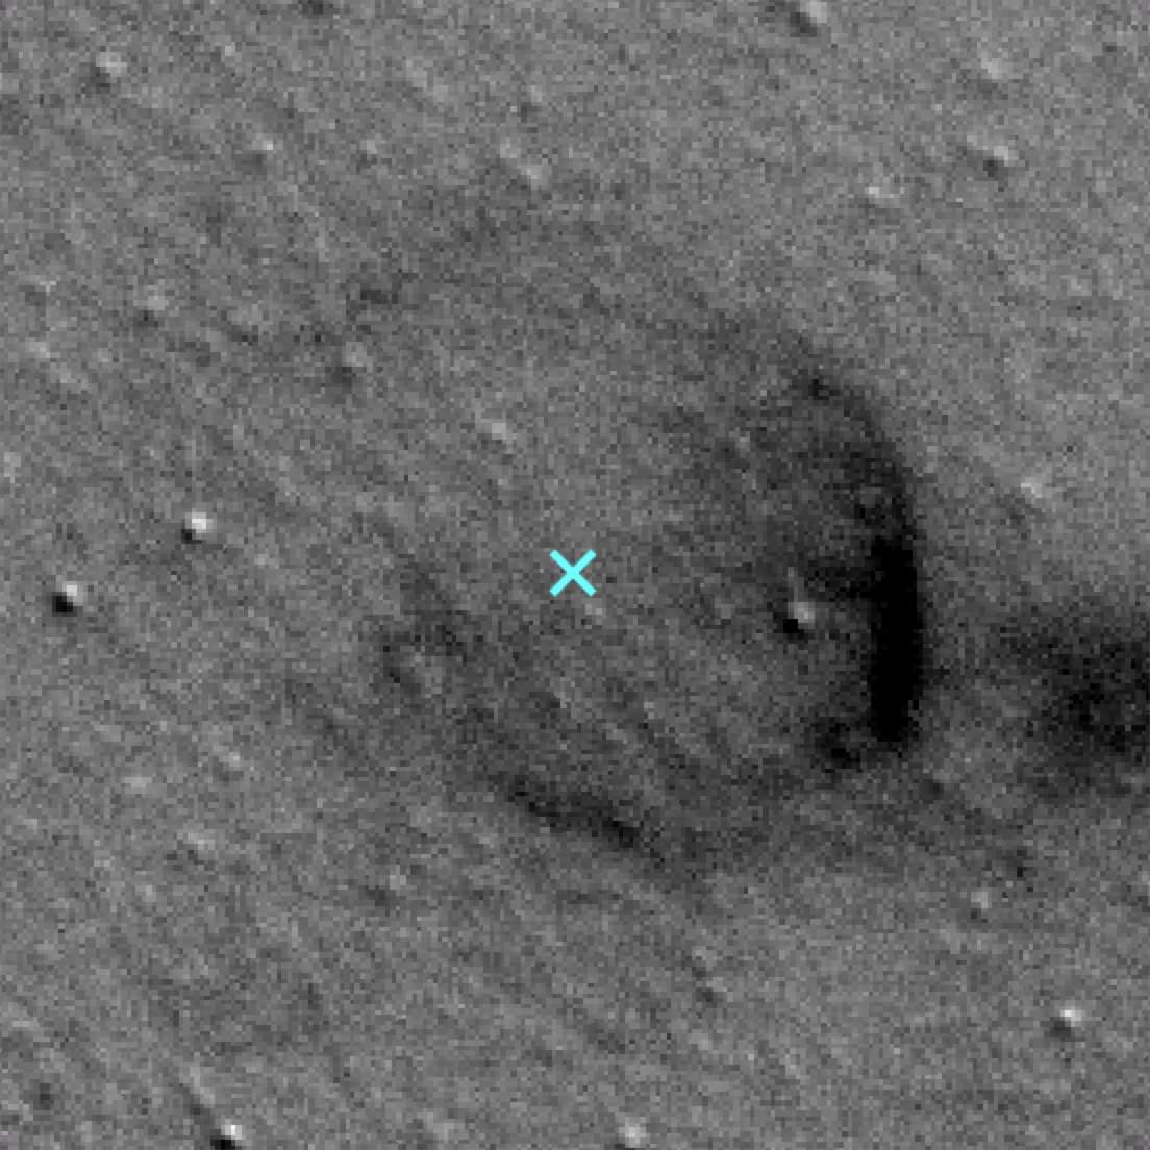
\includegraphics[width=.32\textwidth]{Figures/LGGS_2008_12a_Ha_sub_inverted_without_text.pdf}} \quad
\subfloat{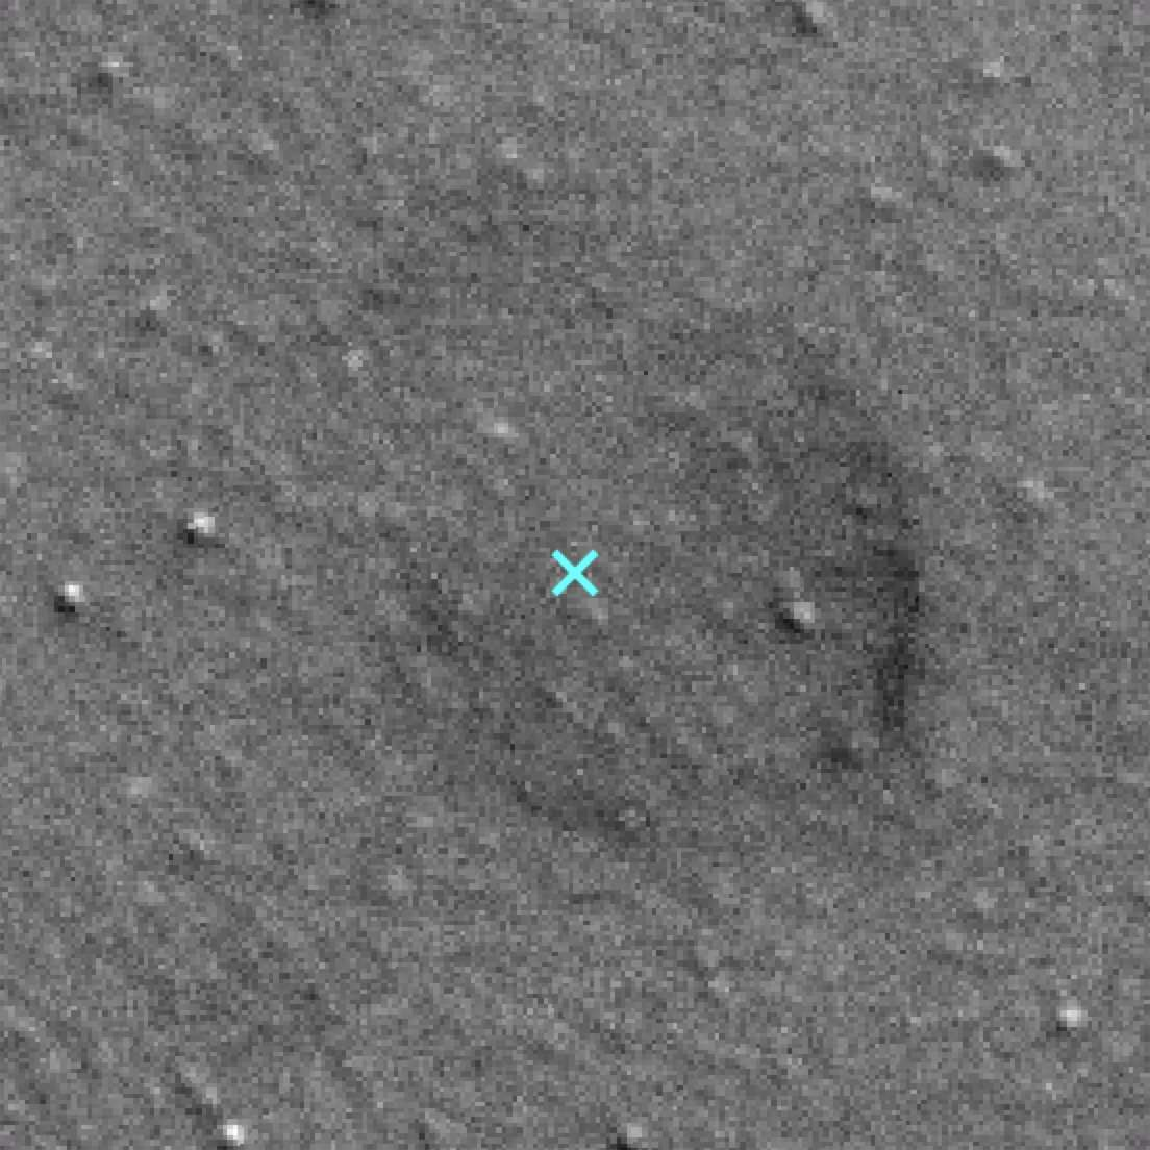
\includegraphics[width=.32\textwidth]{Figures/LGGS_2008_12a_SII_sub_inverted_without_text.pdf}} \quad
\subfloat{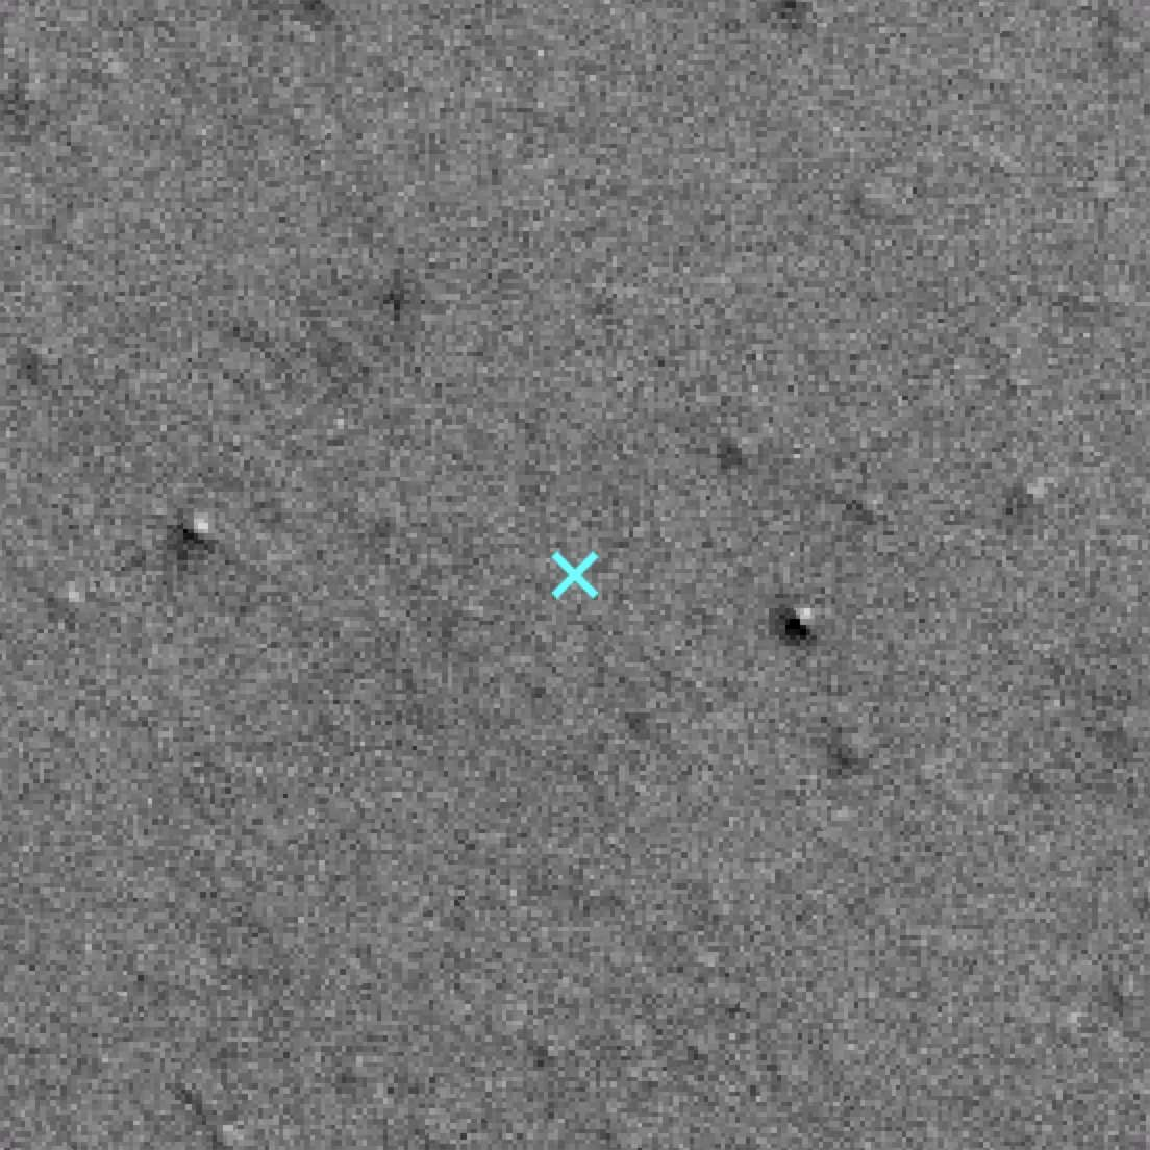
\includegraphics[width=.32\textwidth]{Figures/LGGS_2008_12a_OIII_sub_inverted_without_text.pdf}}
\caption{{\bf -- M\,31N 2008-12a}. The location of the nova (in field 3) is indicated by the blue cross. Left:\ Continuum subtracted LGGS H$\alpha$. Middle:\ Continuum subtracted LGGS [\ion{S}{ii}]. Right:\ Continuum subtracted LGGS [\ion{O}{iii}].}
\label{2008-12a surrounding sub images}
\end{figure*}

\begin{figure*}
\centering
\subfloat{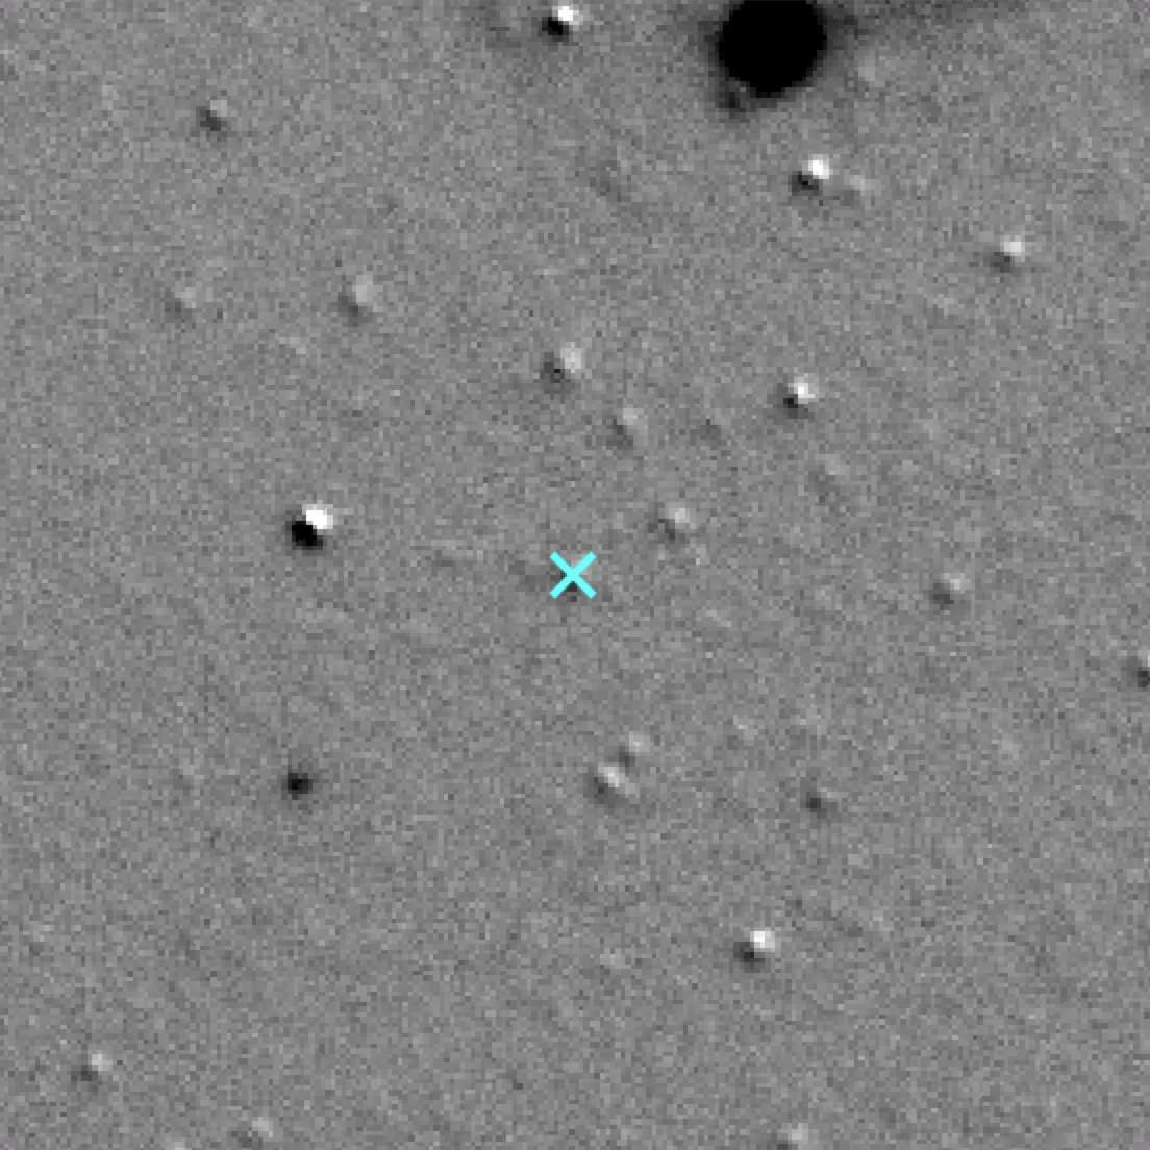
\includegraphics[width=.32\textwidth]{Figures/LGGS_2017_01e_Ha_sub_inverted_without_text.pdf}} \quad
\subfloat{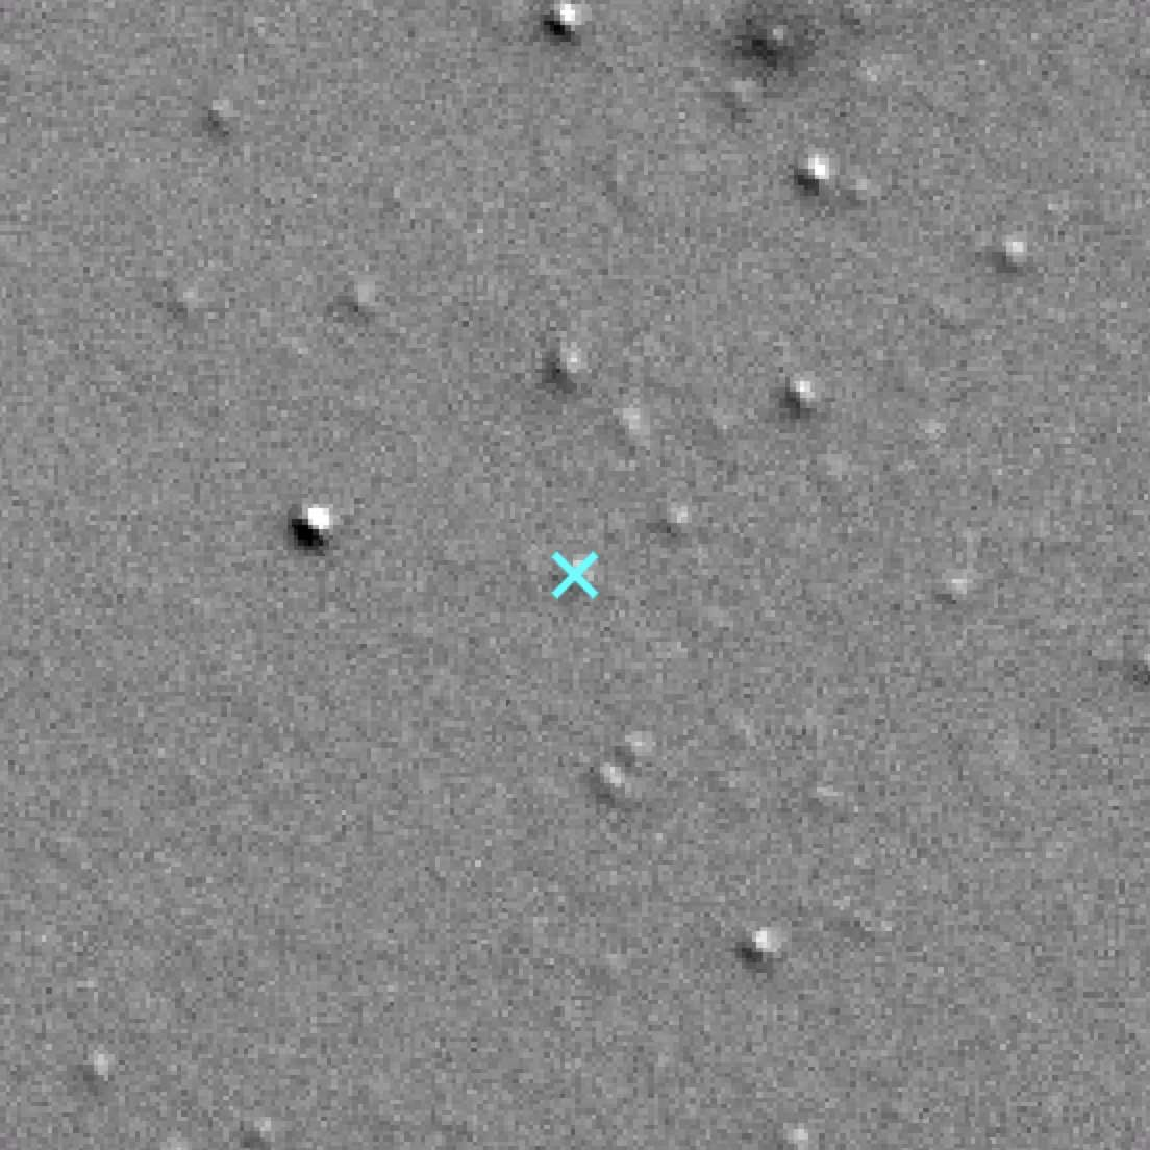
\includegraphics[width=.32\textwidth]{Figures/LGGS_2017_01e_SII_sub_inverted_without_text.pdf}} \quad
\subfloat{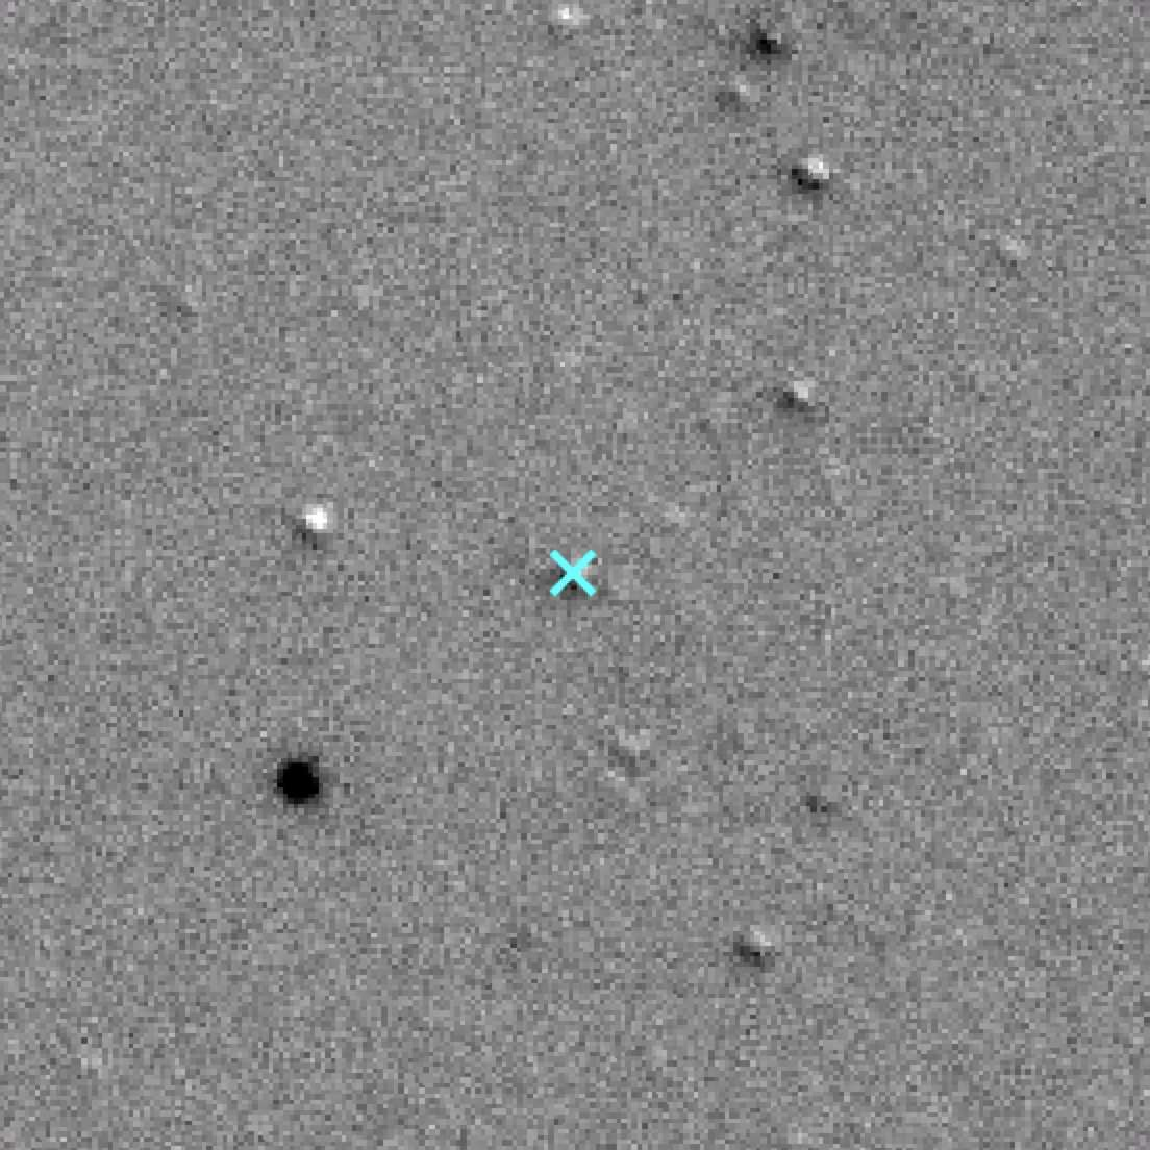
\includegraphics[width=.32\textwidth]{Figures/LGGS_2017_01e_OIII_sub_inverted_without_text.pdf}}
\caption{{\bf -- M\,31N 2017-01e}. The location of the nova (in field 3) is indicated by the blue cross. Left:\ Continuum subtracted LGGS H$\alpha$. Middle:\ Continuum subtracted LGGS [\ion{S}{ii}]. Right:\ Continuum subtracted LGGS [\ion{O}{iii}].}
\label{2017-01e surrounding sub images}
\end{figure*}

\begin{figure*}
\centering
\subfloat{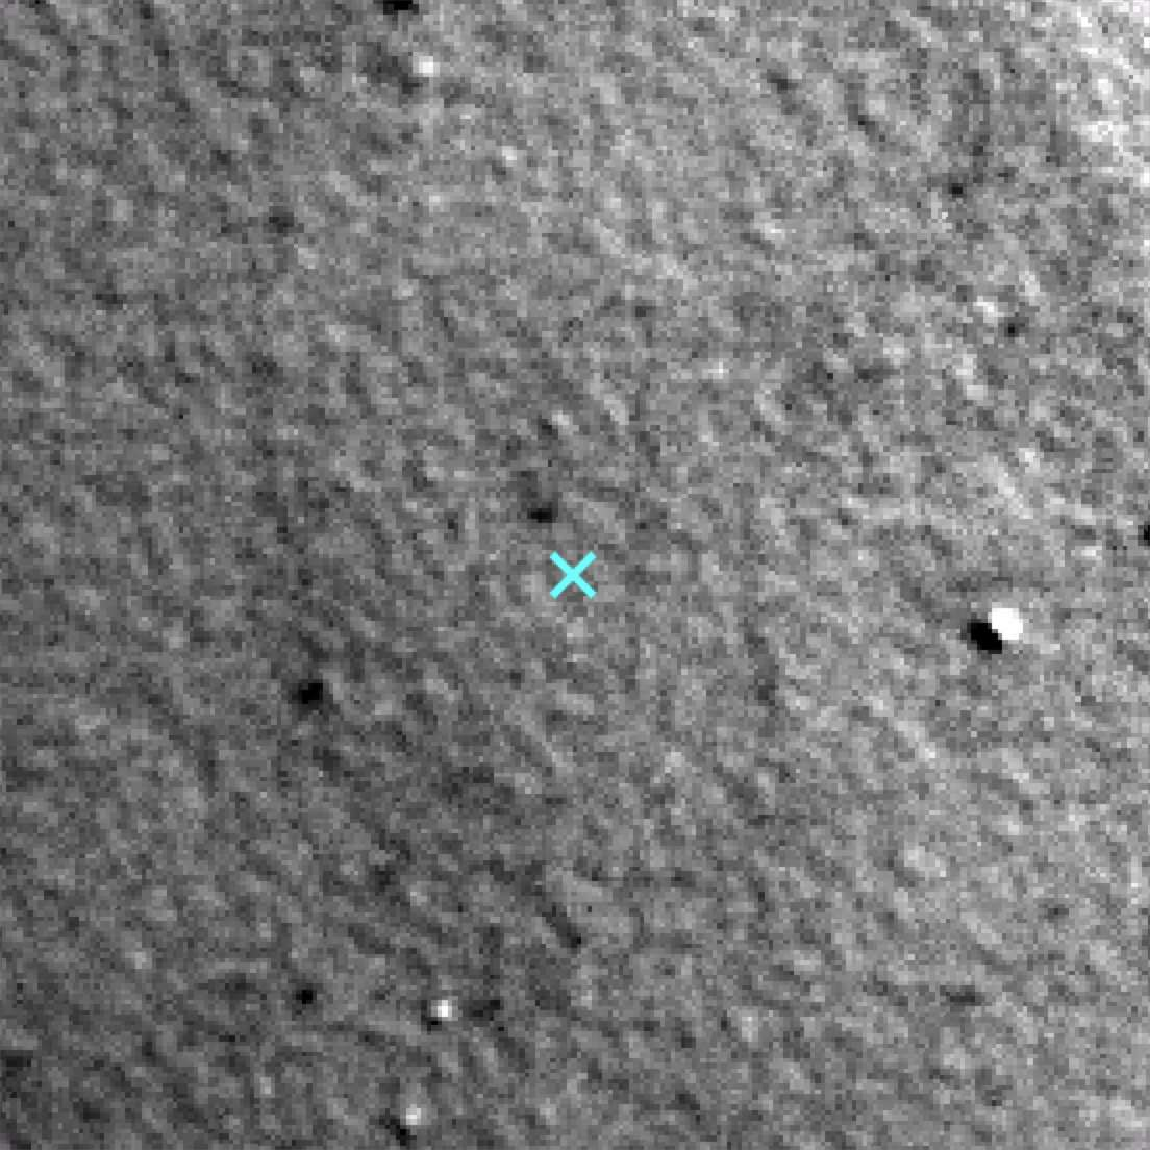
\includegraphics[width=.32\textwidth]{Figures/LGGS_1926_07c_Ha_sub_inverted_without_text.pdf}} \quad
\subfloat{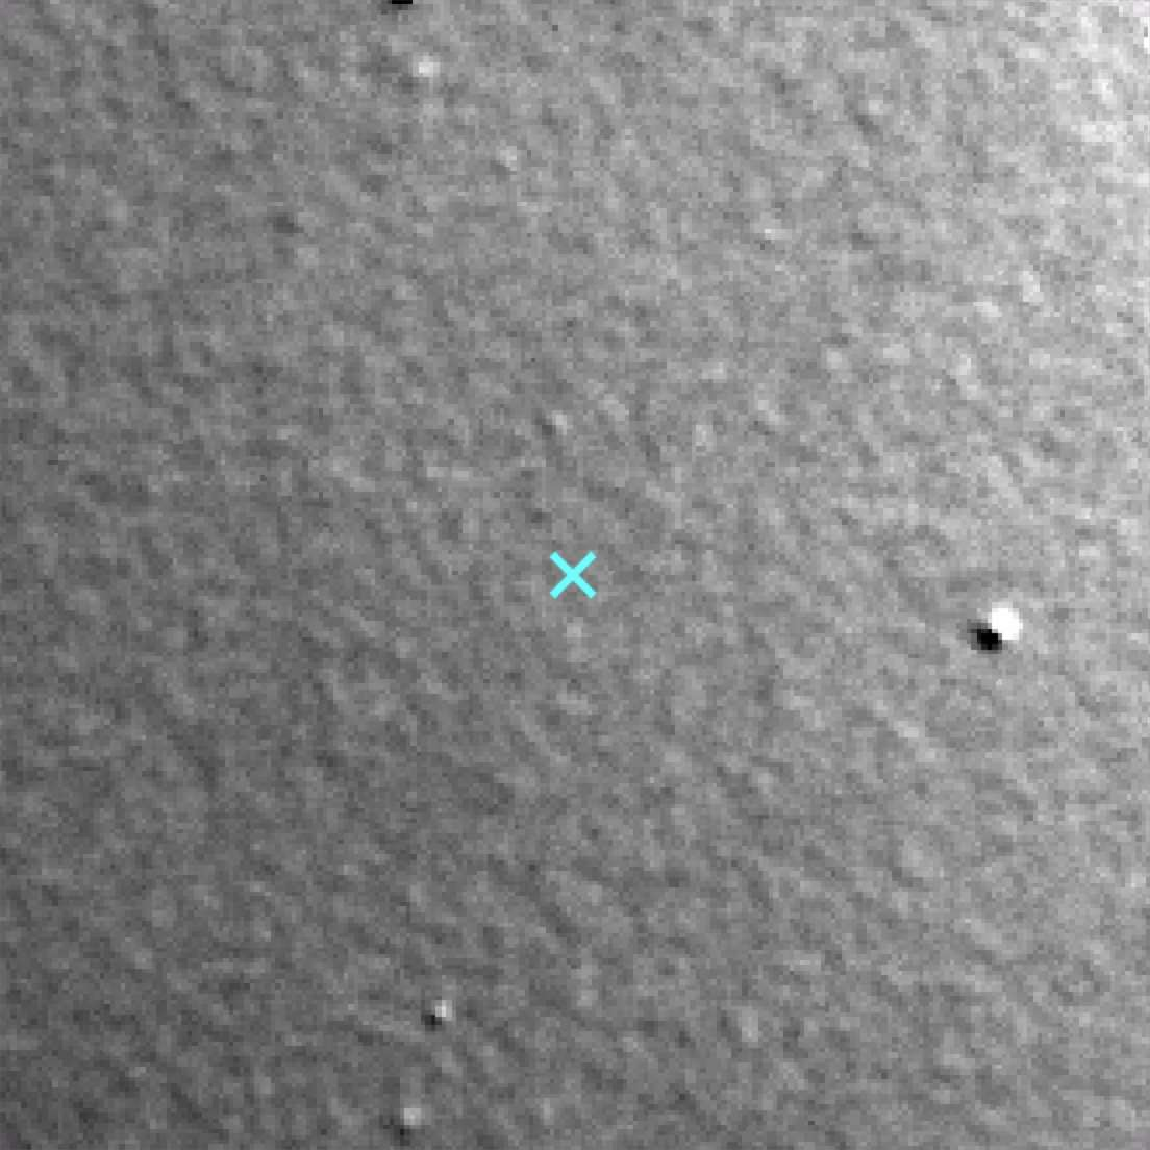
\includegraphics[width=.32\textwidth]{Figures/LGGS_1926_07c_SII_sub_inverted_without_text.pdf}} \quad
\subfloat{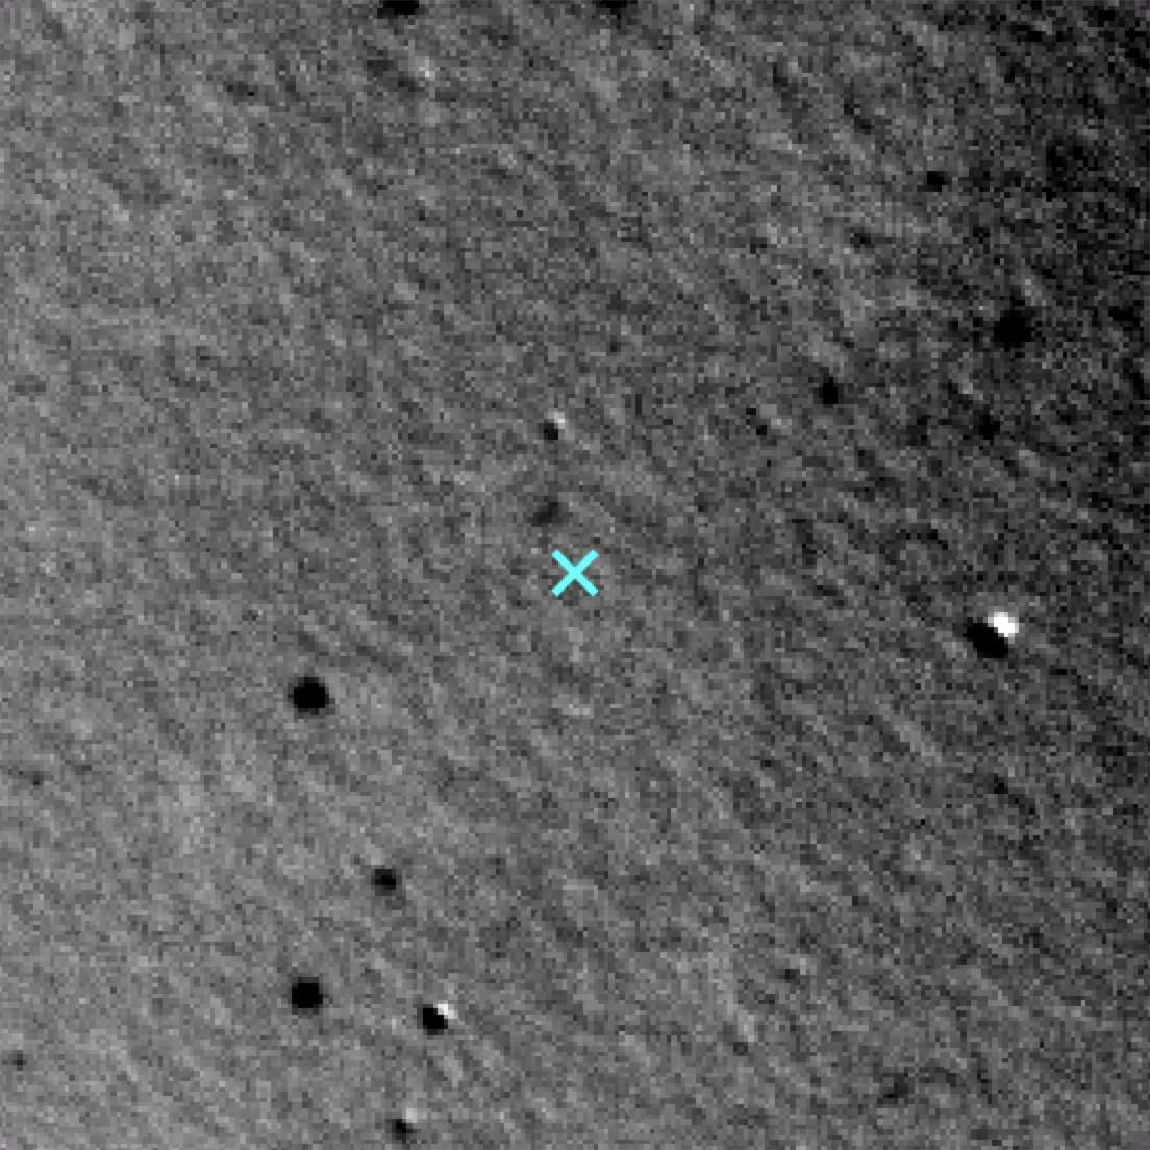
\includegraphics[width=.32\textwidth]{Figures/LGGS_1926_07c_OIII_sub_inverted_without_text.pdf}}
\caption{{\bf -- M\,31N 1926-07c}. The location of the nova (in field 6) is indicated by the blue cross. Left:\ Continuum subtracted LGGS H$\alpha$. Middle:\ Continuum subtracted LGGS [\ion{S}{ii}]. Right:\ Continuum subtracted LGGS [\ion{O}{iii}].}
\label{1926-07c surrounding sub images}
\end{figure*}

\begin{figure*}
\centering
\subfloat{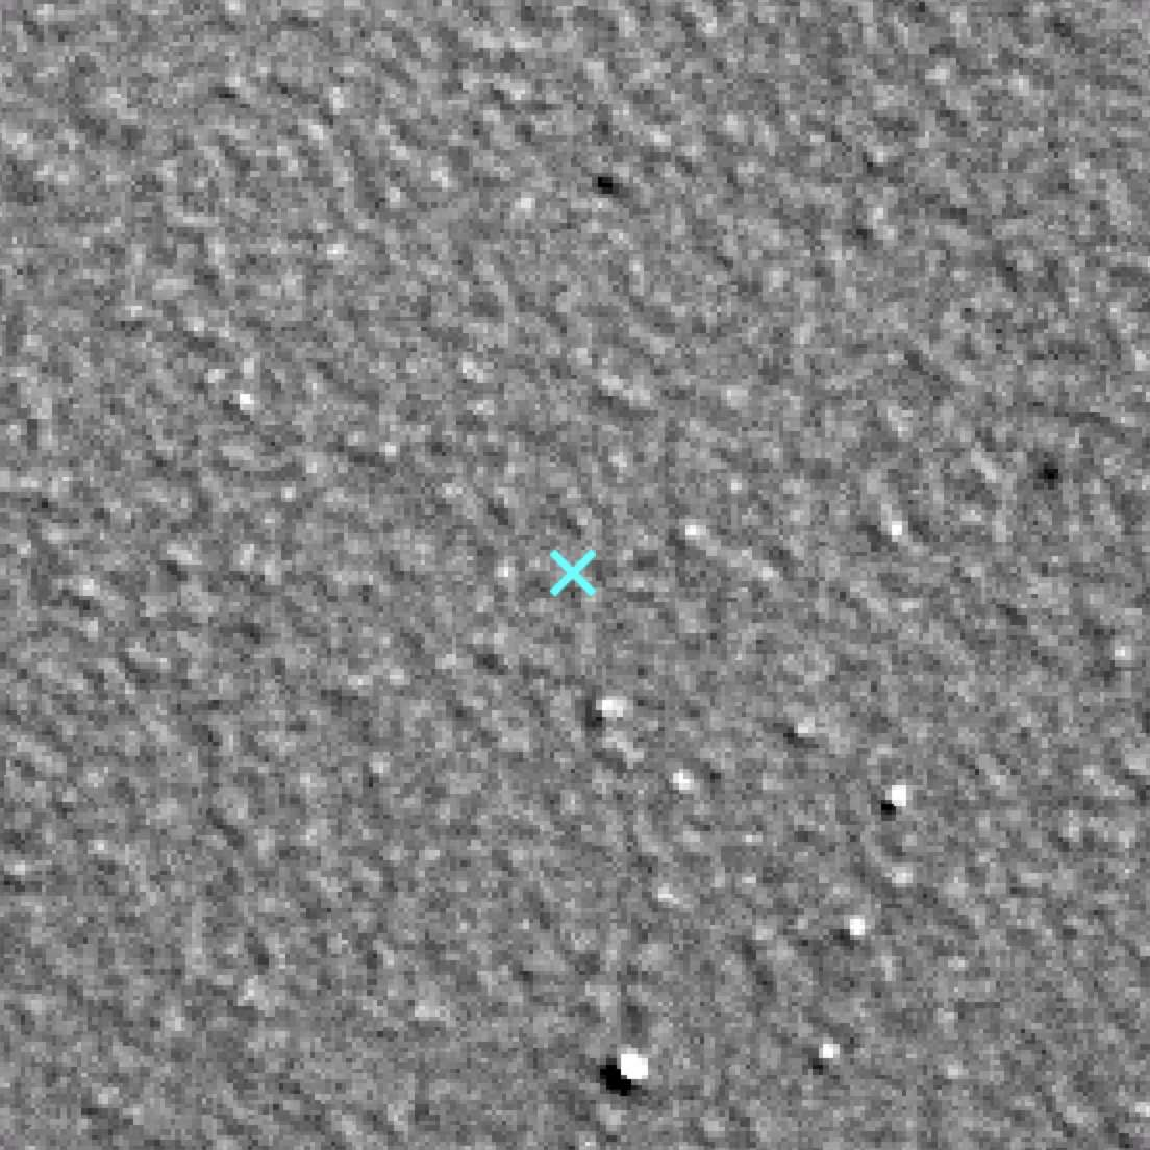
\includegraphics[width=.32\textwidth]{Figures/LGGS_1997_11k_Ha_sub_inverted_without_text.pdf}} \quad
\subfloat{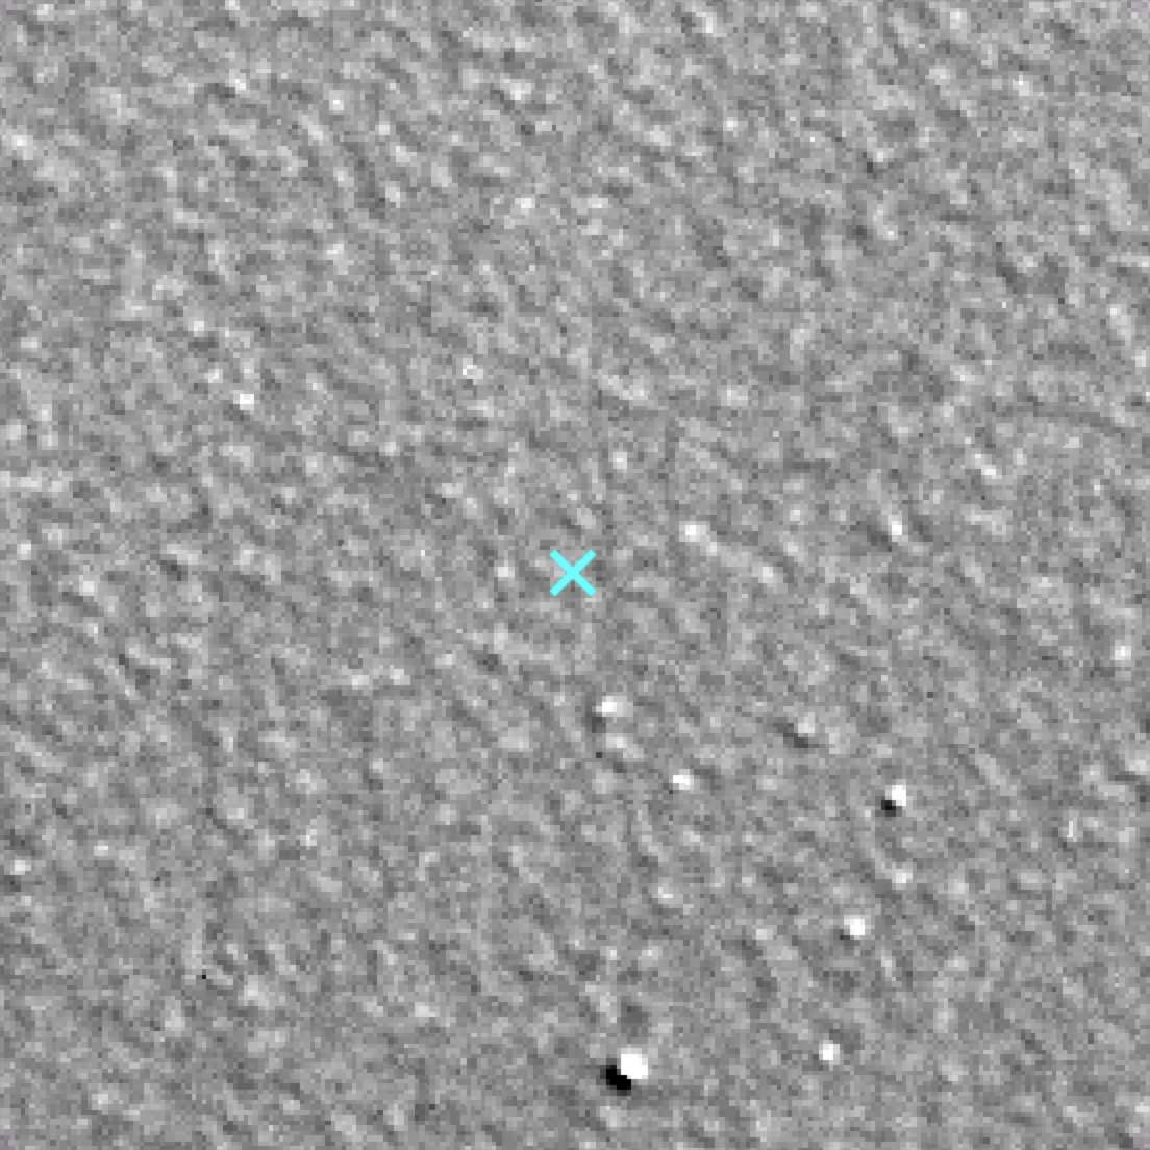
\includegraphics[width=.32\textwidth]{Figures/LGGS_1997_11k_SII_sub_inverted_without_text.pdf}} \quad
\subfloat{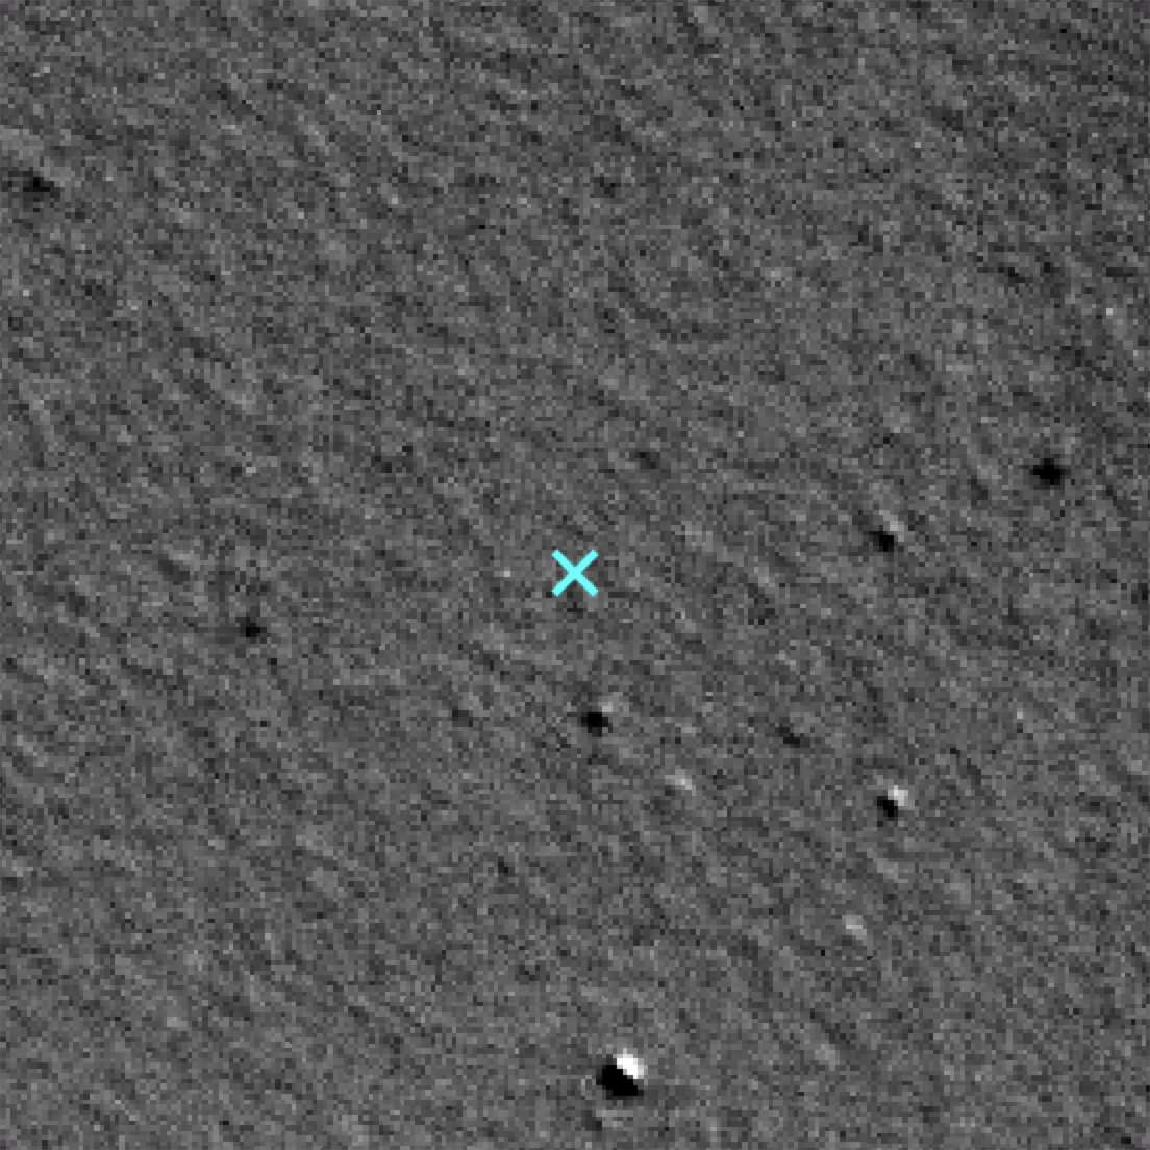
\includegraphics[width=.32\textwidth]{Figures/LGGS_1997_11k_OIII_sub_inverted_without_text.pdf}}
\caption{{\bf -- M\,31N 1997-11k}. The location of the nova (in field 6) is indicated by the blue cross. Left:\ Continuum subtracted LGGS H$\alpha$. Middle:\ Continuum subtracted LGGS [\ion{S}{ii}]. Right:\ Continuum subtracted LGGS [\ion{O}{iii}].}
\label{1997-11k surrounding sub images}
\end{figure*}

\begin{figure*}
\centering
\subfloat{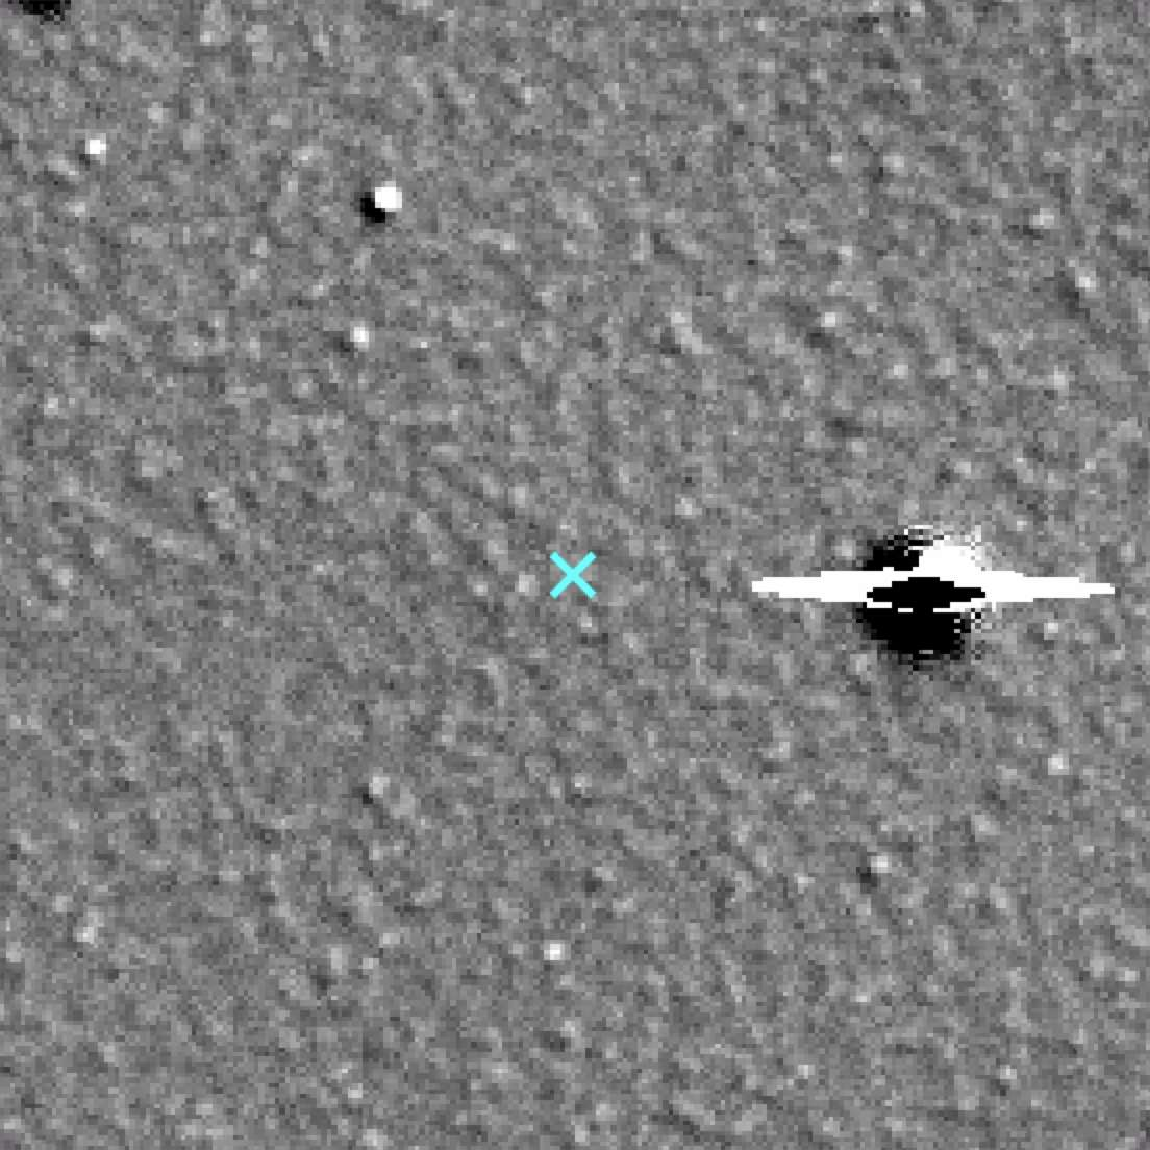
\includegraphics[width=.32\textwidth]{Figures/LGGS_1963_09c_Ha_sub_inverted_without_text.pdf}} \quad
\subfloat{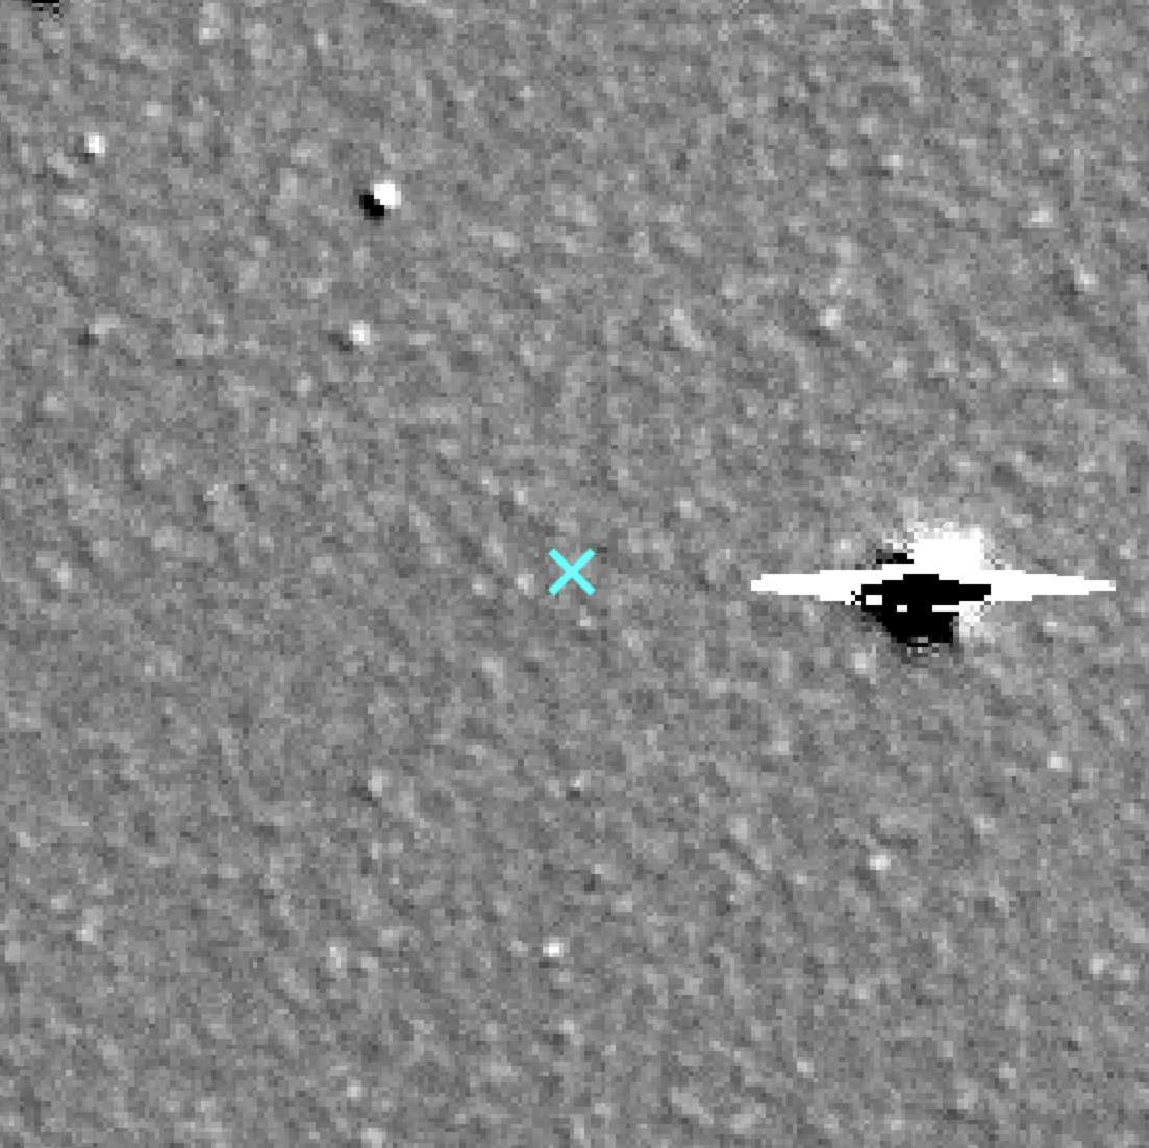
\includegraphics[width=.32\textwidth]{Figures/LGGS_1963_09c_SII_sub_inverted_without_text.pdf}} \quad
\subfloat{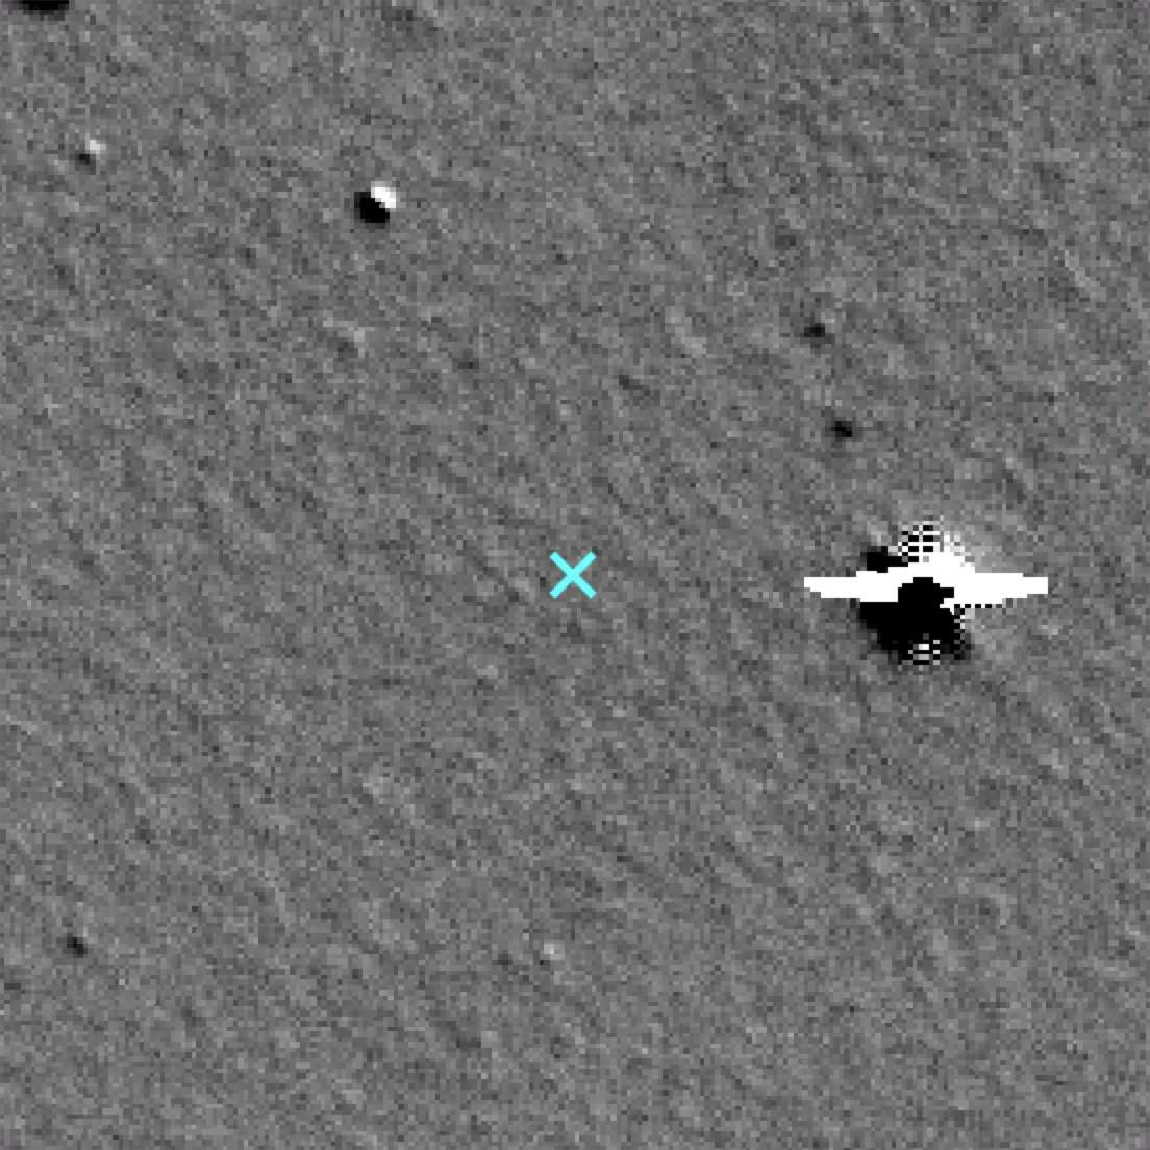
\includegraphics[width=.32\textwidth]{Figures/LGGS_1963_09c_OIII_sub_inverted_without_text.pdf}}
\caption{{\bf -- M\,31N 1963-09c}. The location of the nova (in field 6) is indicated by the blue cross. Left:\ Continuum subtracted LGGS H$\alpha$. Middle:\ Continuum subtracted LGGS [\ion{S}{ii}]. Right:\ Continuum subtracted LGGS [\ion{O}{iii}].}
\label{1963-09c surrounding sub images}
\end{figure*}

\begin{figure*}
\centering
\subfloat{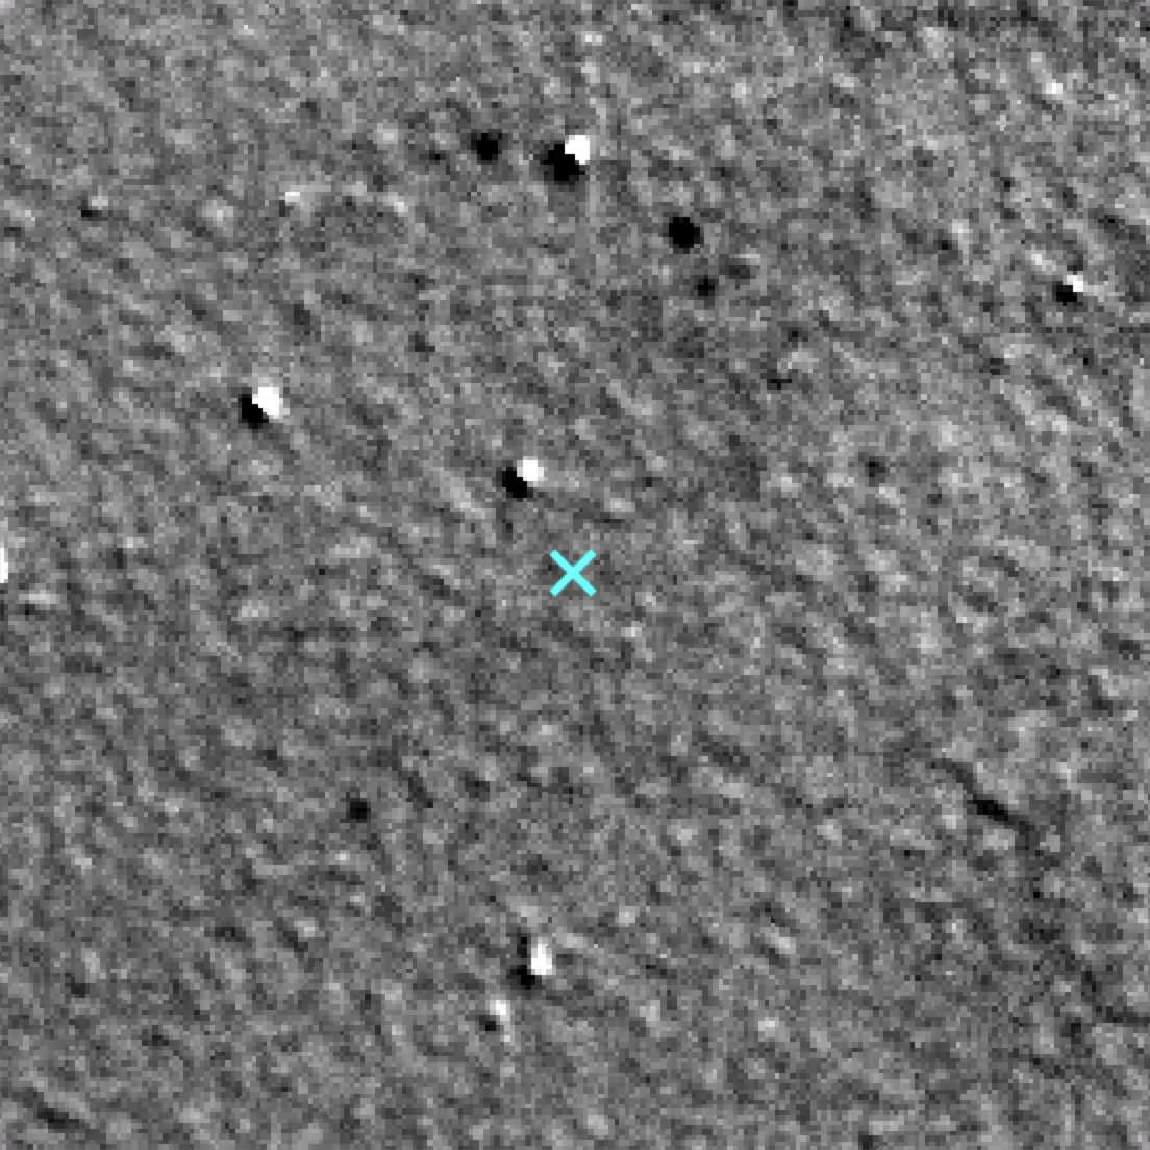
\includegraphics[width=.32\textwidth]{Figures/LGGS_1960_12a_Ha_sub_inverted_without_text.pdf}} \quad
\subfloat{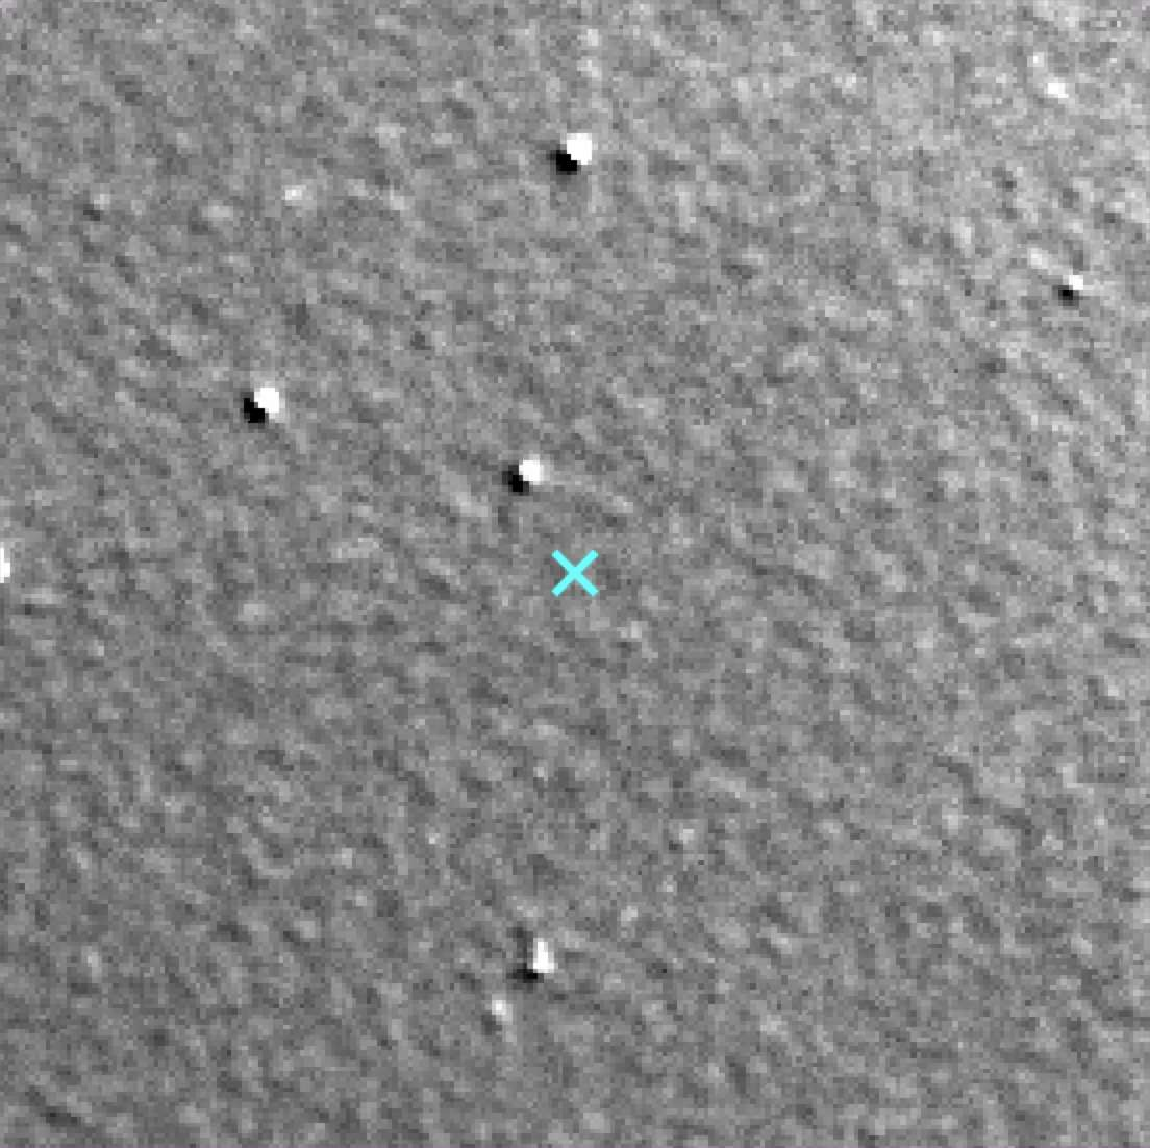
\includegraphics[width=.32\textwidth]{Figures/LGGS_1960_12a_SII_sub_inverted_without_text.pdf}} \quad
\subfloat{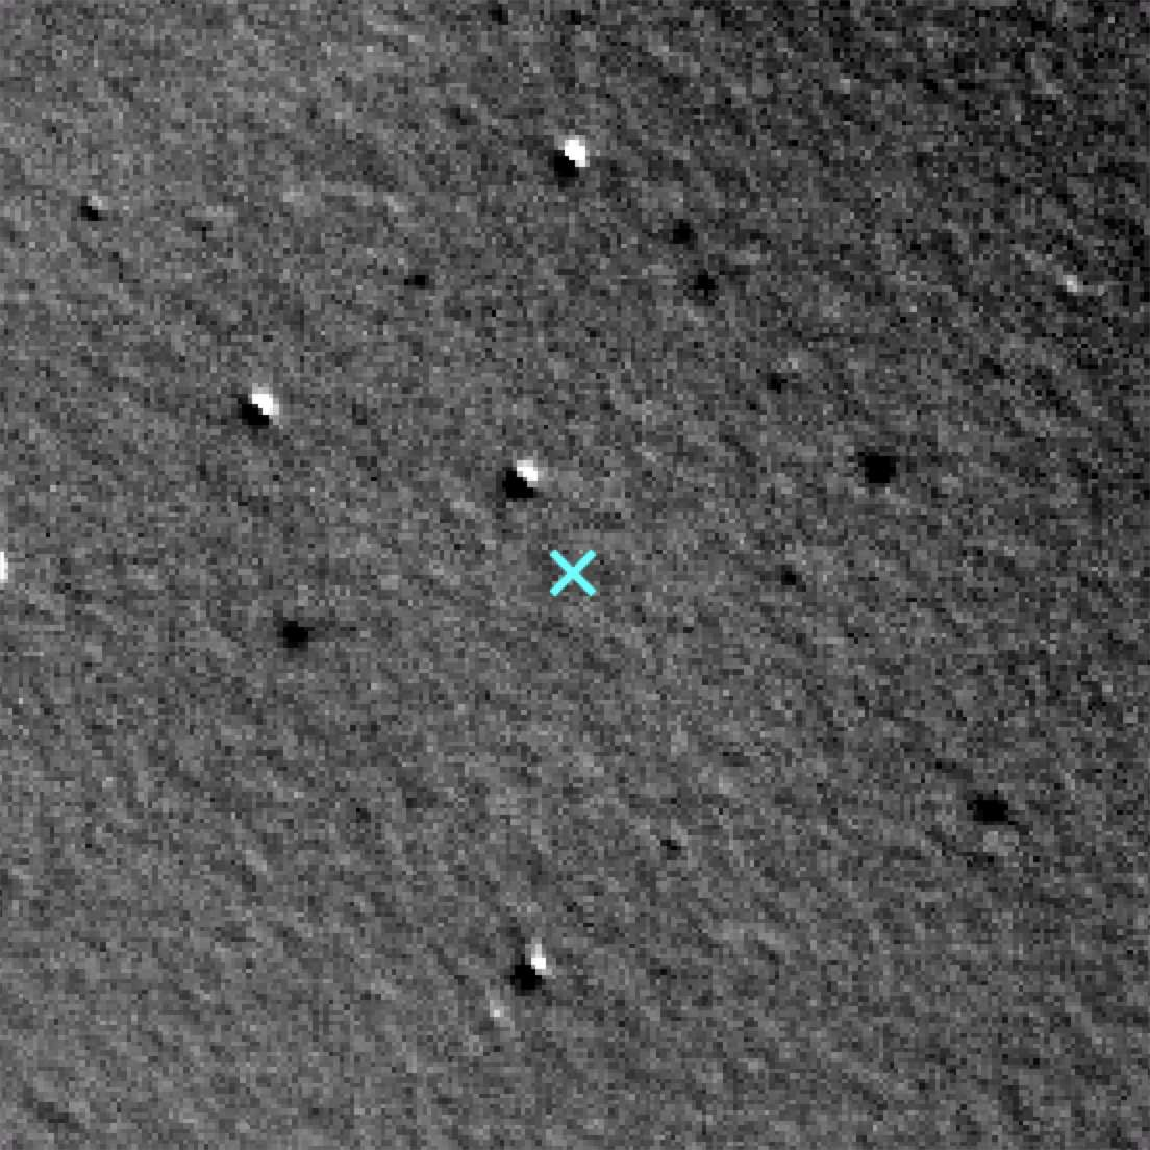
\includegraphics[width=.32\textwidth]{Figures/LGGS_1960_12a_OIII_sub_inverted_without_text.pdf}}
\caption{{\bf -- M\,31N 1960-12a}. The location of the nova (in field 6) is indicated by the blue cross. Left:\ Continuum subtracted LGGS H$\alpha$. Middle:\ Continuum subtracted LGGS [\ion{S}{ii}]. Right:\ Continuum subtracted LGGS [\ion{O}{iii}].}
\label{1960-12a surrounding sub images}
\end{figure*}

\begin{figure*}
\centering
\subfloat{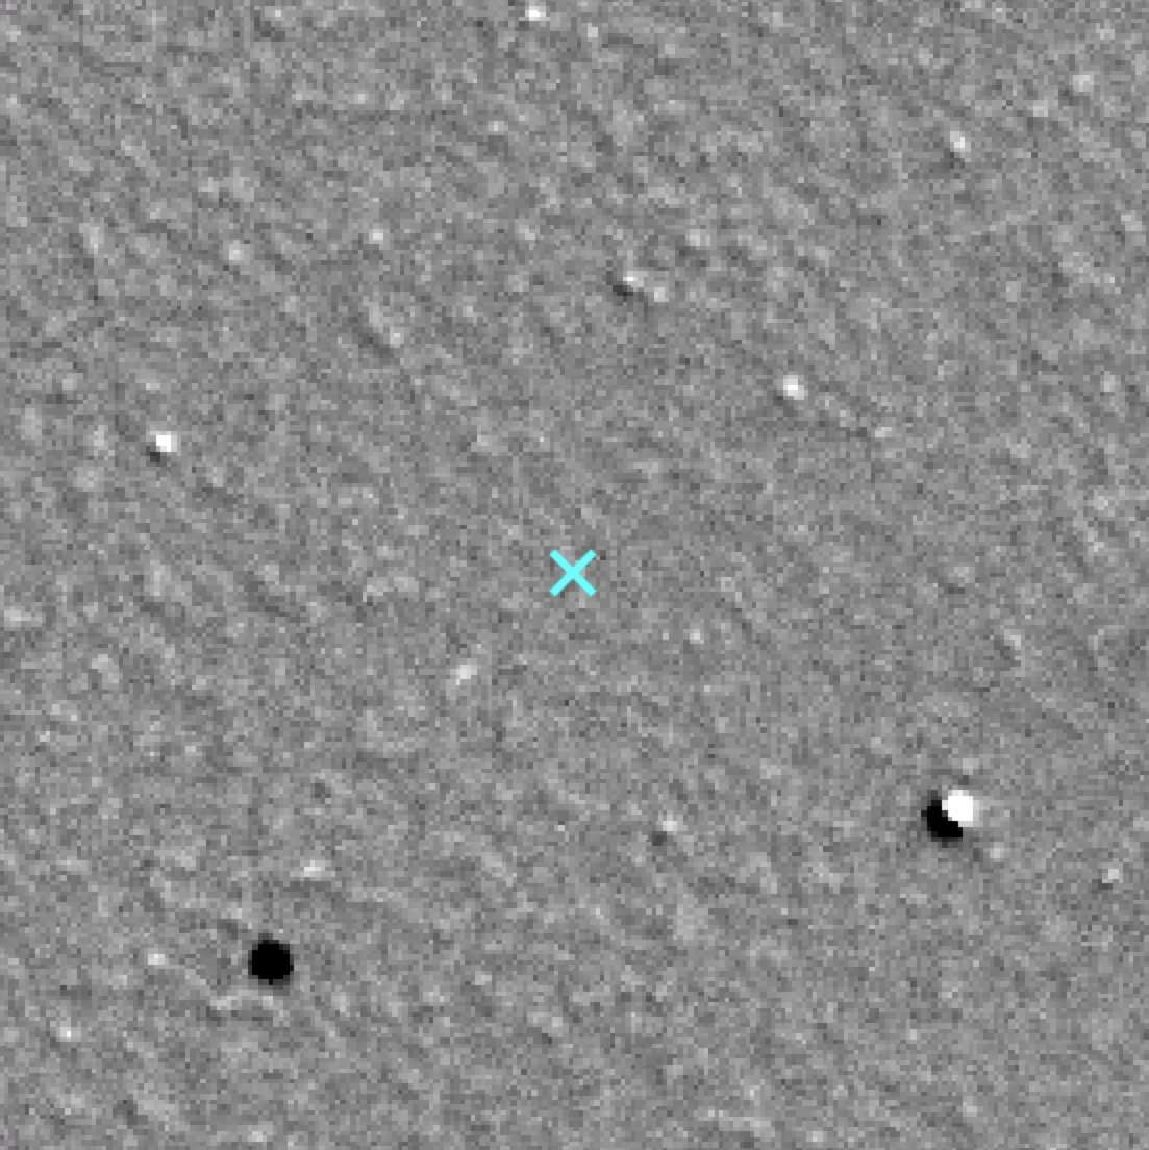
\includegraphics[width=.32\textwidth]{Figures/LGGS_2006_11c_Ha_sub_inverted_without_text.pdf}} \quad
\subfloat{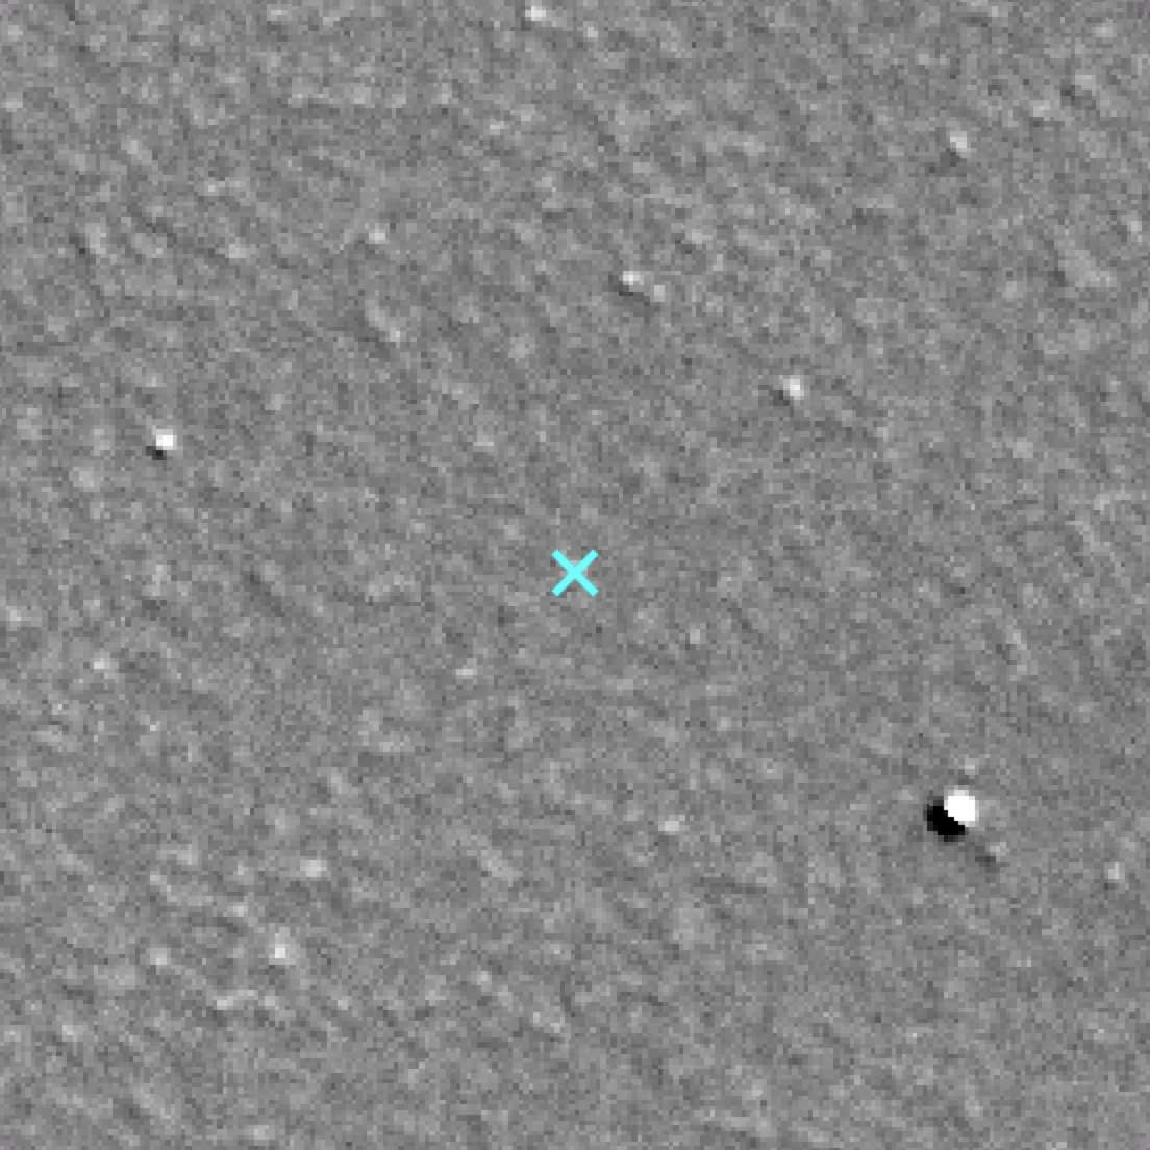
\includegraphics[width=.32\textwidth]{Figures/LGGS_2006_11c_SII_sub_inverted_without_text.pdf}} \quad
\subfloat{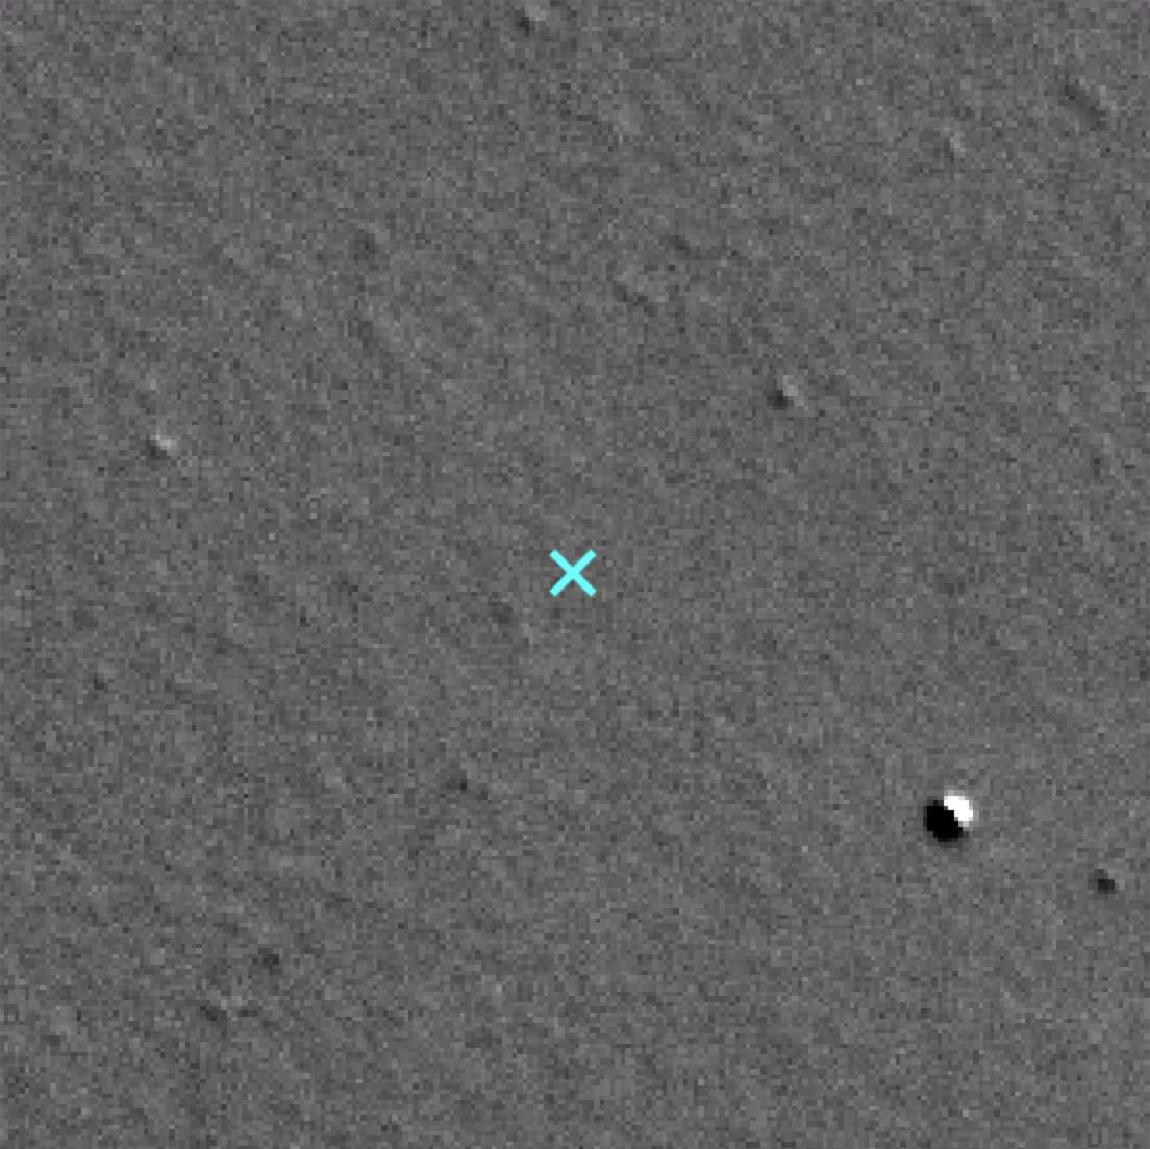
\includegraphics[width=.32\textwidth]{Figures/LGGS_2006_11c_OIII_sub_inverted_without_text.pdf}}
\caption{{\bf -- M\,31N 2006-11c}. The location of the nova (in field 6) is indicated by the blue cross. Left:\ Continuum subtracted LGGS H$\alpha$. Middle:\ Continuum subtracted LGGS [\ion{S}{ii}]. Right:\ Continuum subtracted LGGS [\ion{O}{iii}].}
\label{2006-11c surrounding sub images}
\end{figure*}

\begin{figure*}
\centering
\subfloat{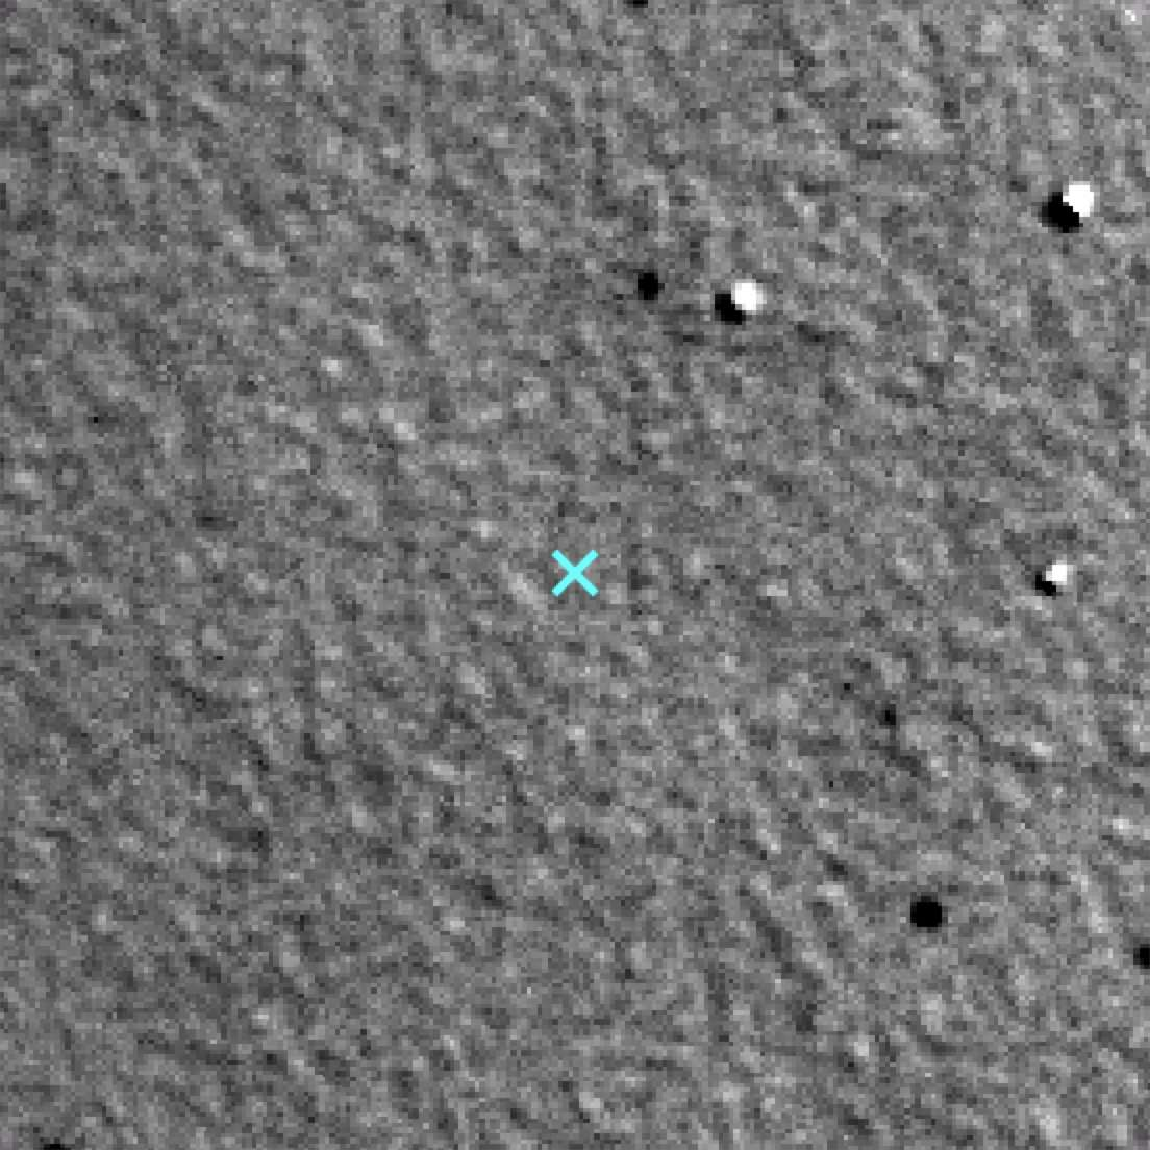
\includegraphics[width=.32\textwidth]{Figures/LGGS_1990_10a_Ha_sub_inverted_without_text.pdf}} \quad
\subfloat{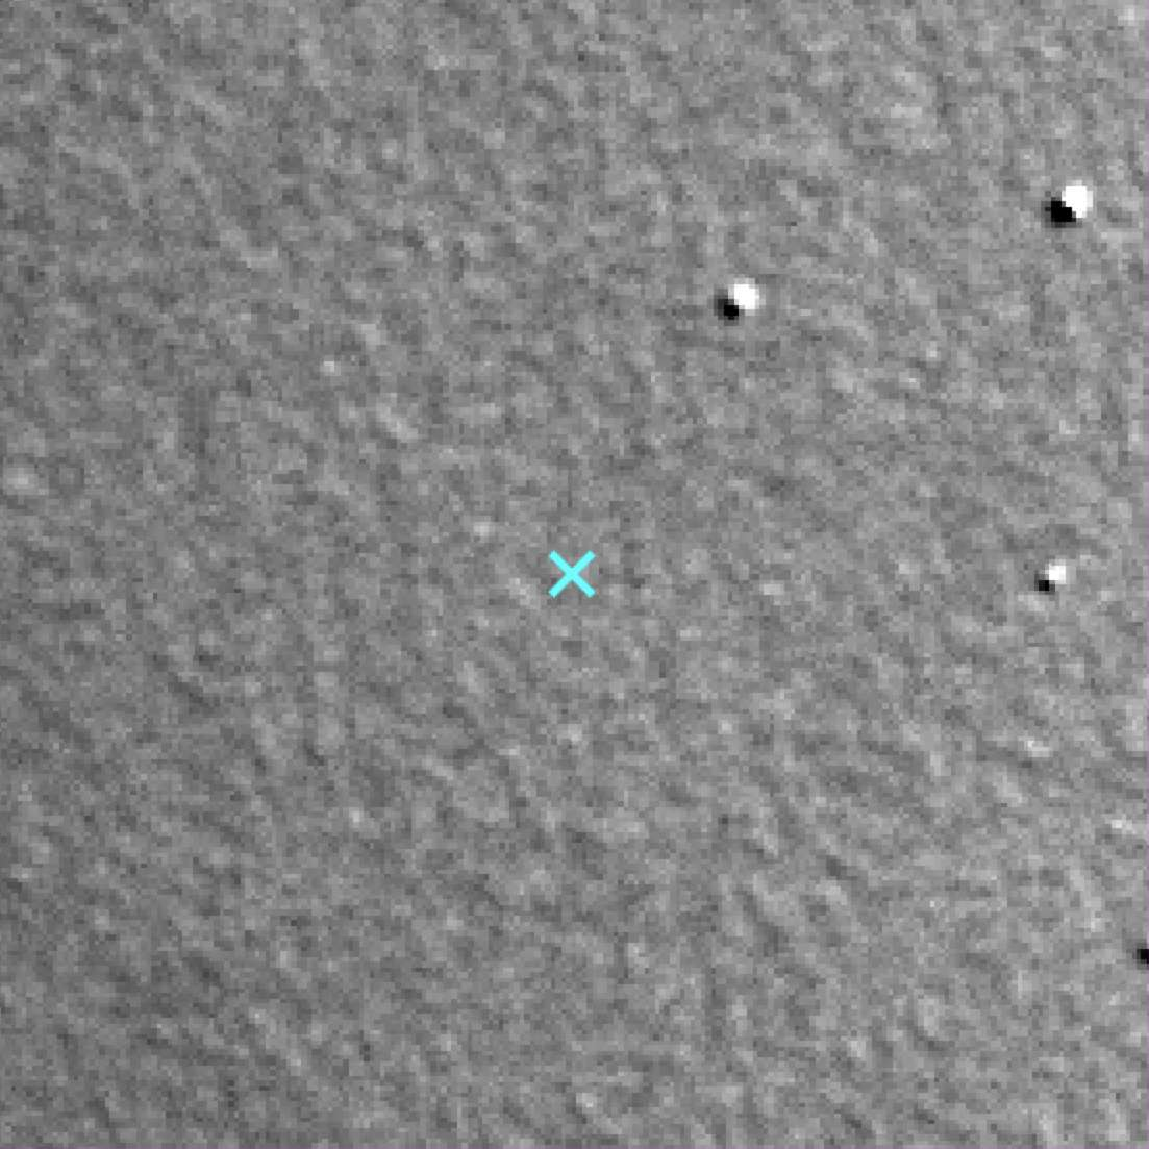
\includegraphics[width=.32\textwidth]{Figures/LGGS_1990_10a_SII_sub_inverted_without_text.pdf}} \quad
\subfloat{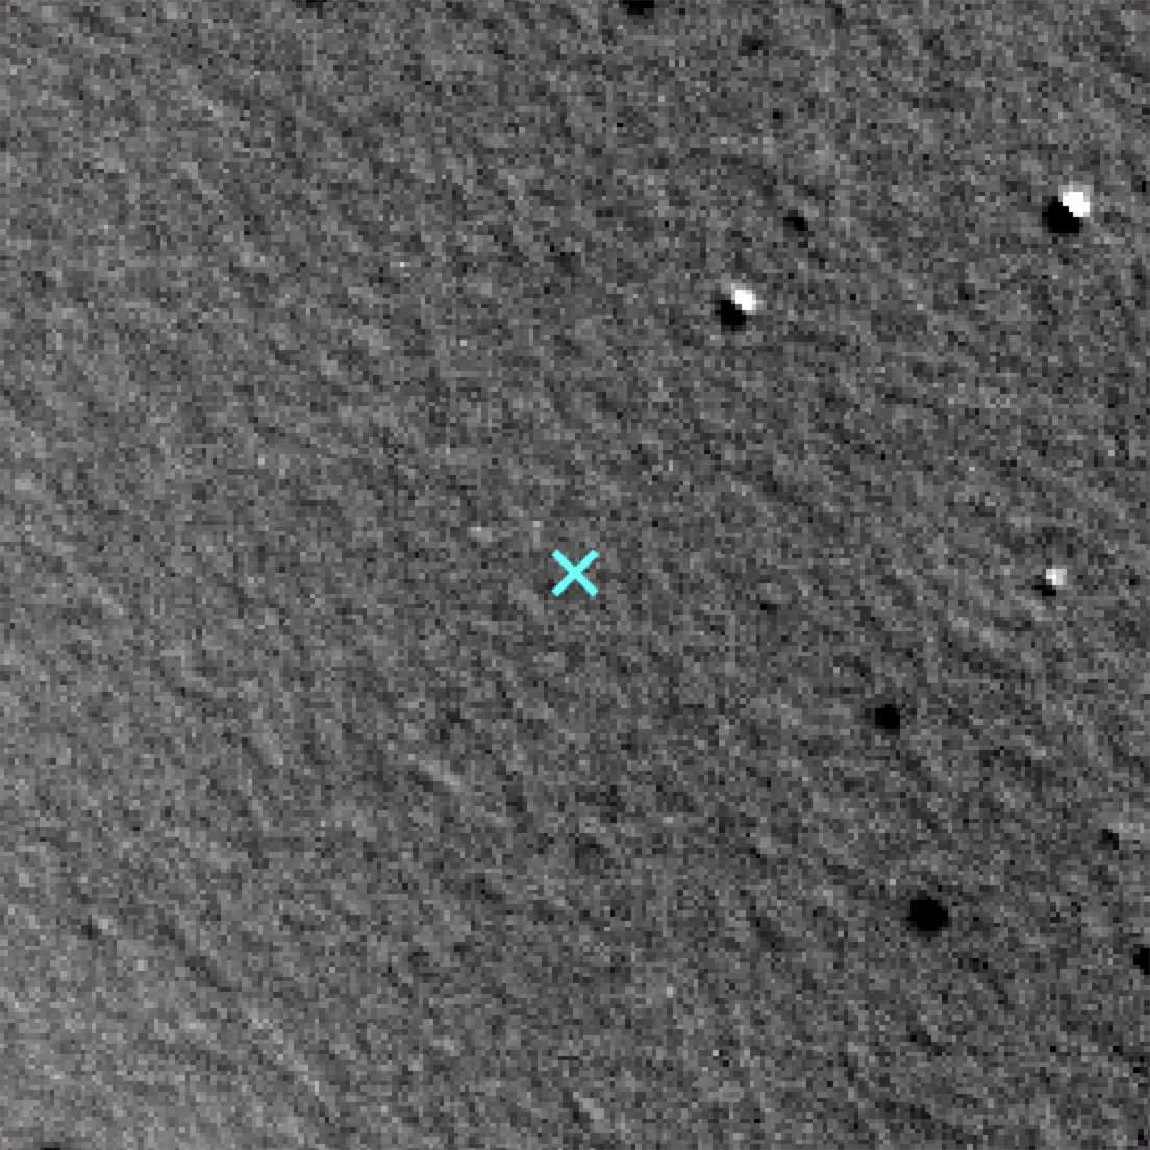
\includegraphics[width=.32\textwidth]{Figures/LGGS_1990_10a_OIII_sub_inverted_without_text.pdf}}
\caption{{\bf -- M\,31N 1990-10a}. The location of the nova (in field 6) is indicated by the blue cross. Left:\ Continuum subtracted LGGS H$\alpha$. Middle:\ Continuum subtracted LGGS [\ion{S}{ii}]. Right:\ Continuum subtracted LGGS [\ion{O}{iii}].}
\label{1990-10a surrounding sub images}
\end{figure*}

\begin{figure*}
\centering
\subfloat{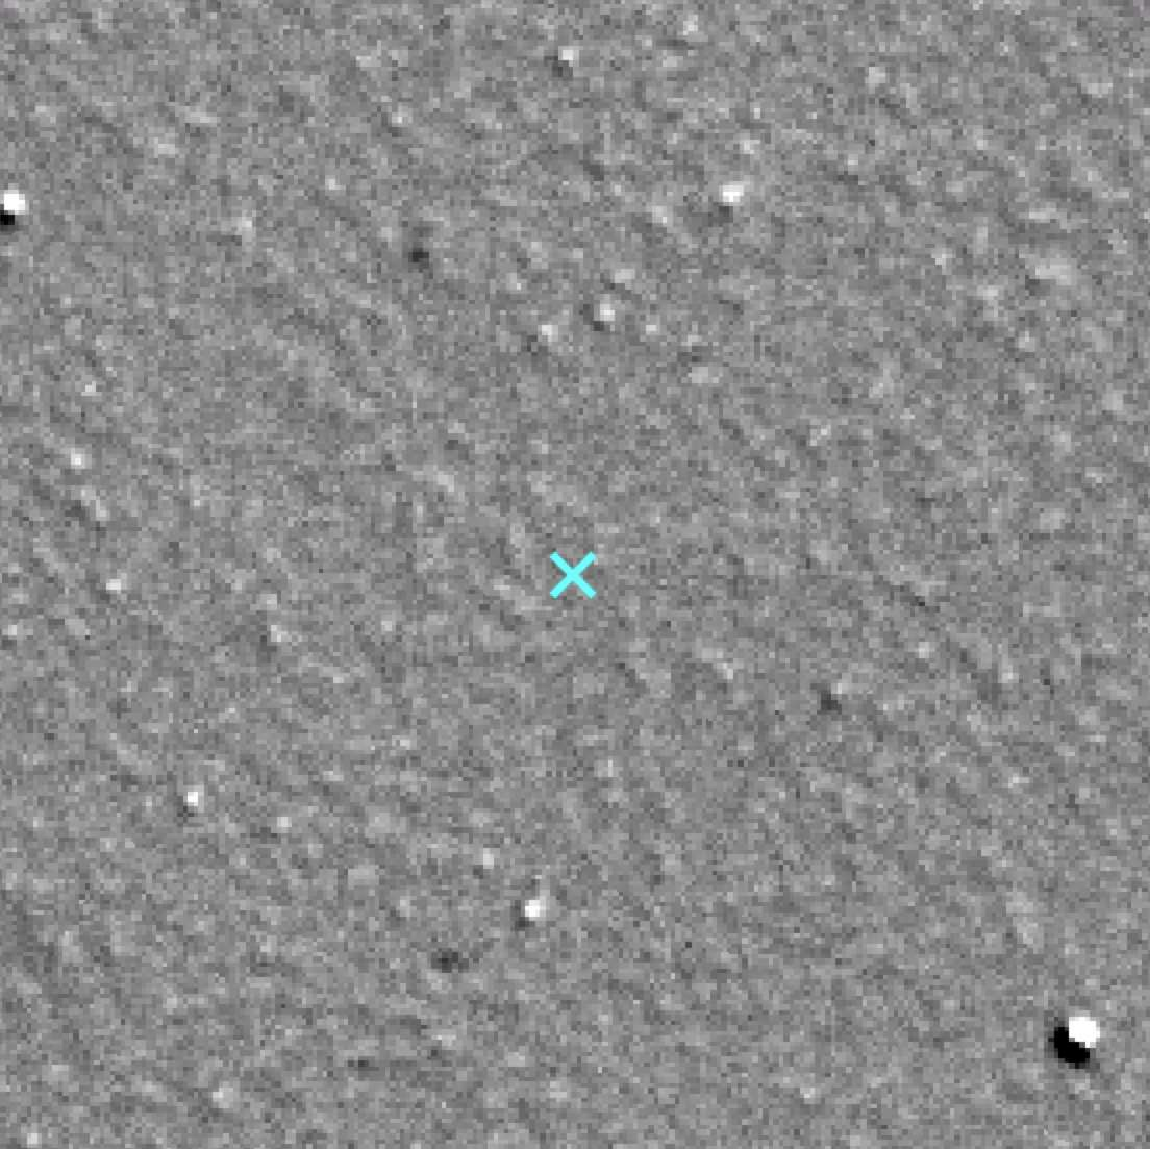
\includegraphics[width=.32\textwidth]{Figures/LGGS_2007_11f_Ha_sub_inverted_without_text.pdf}} \quad
\subfloat{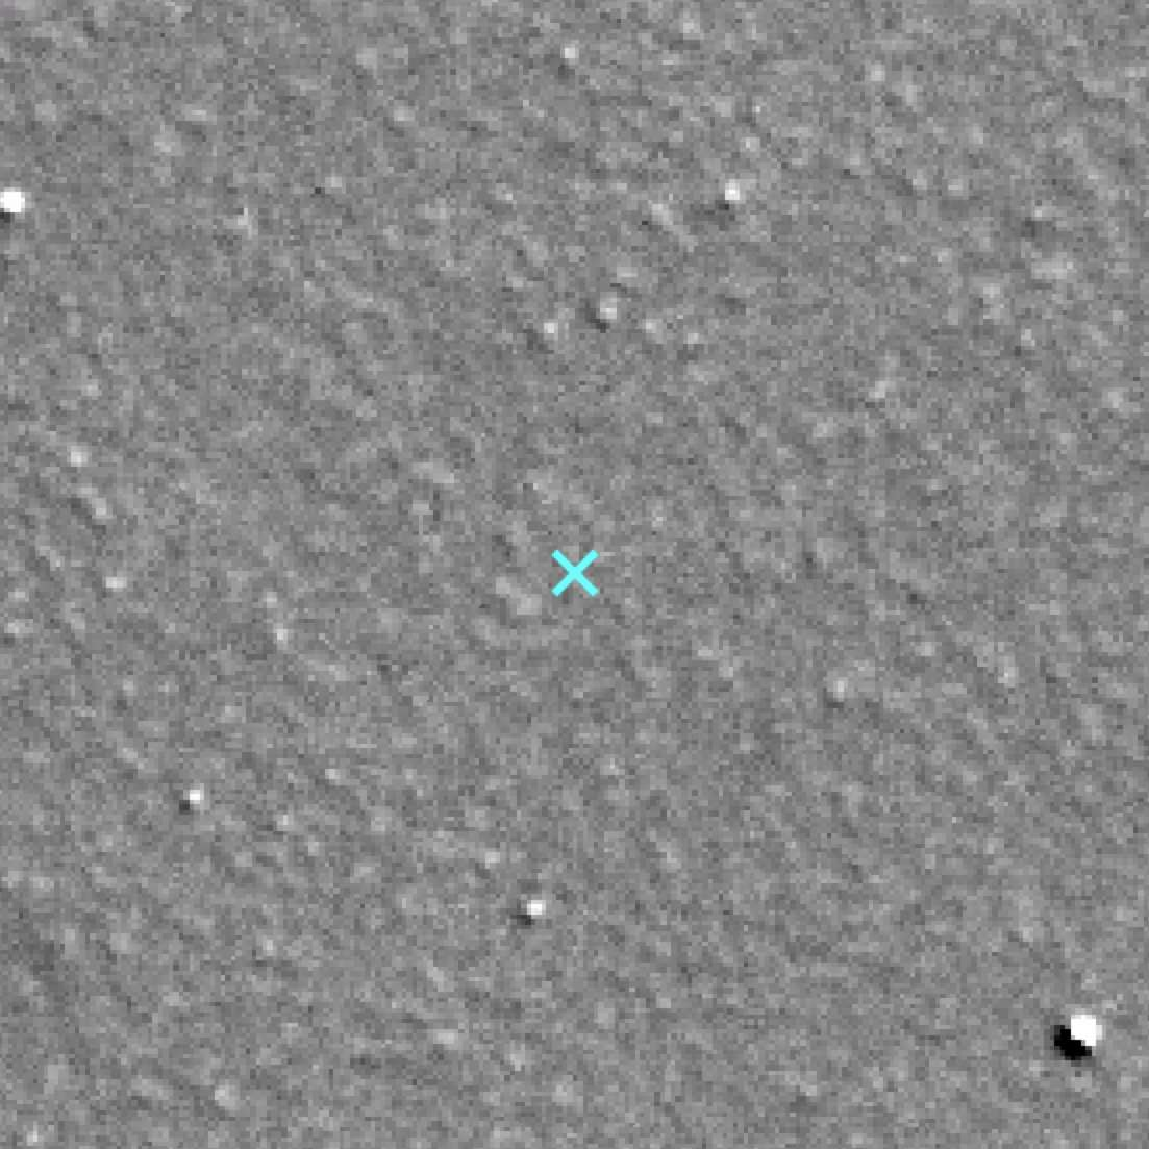
\includegraphics[width=.32\textwidth]{Figures/LGGS_2007_11f_SII_sub_inverted_without_text.pdf}} \quad
\subfloat{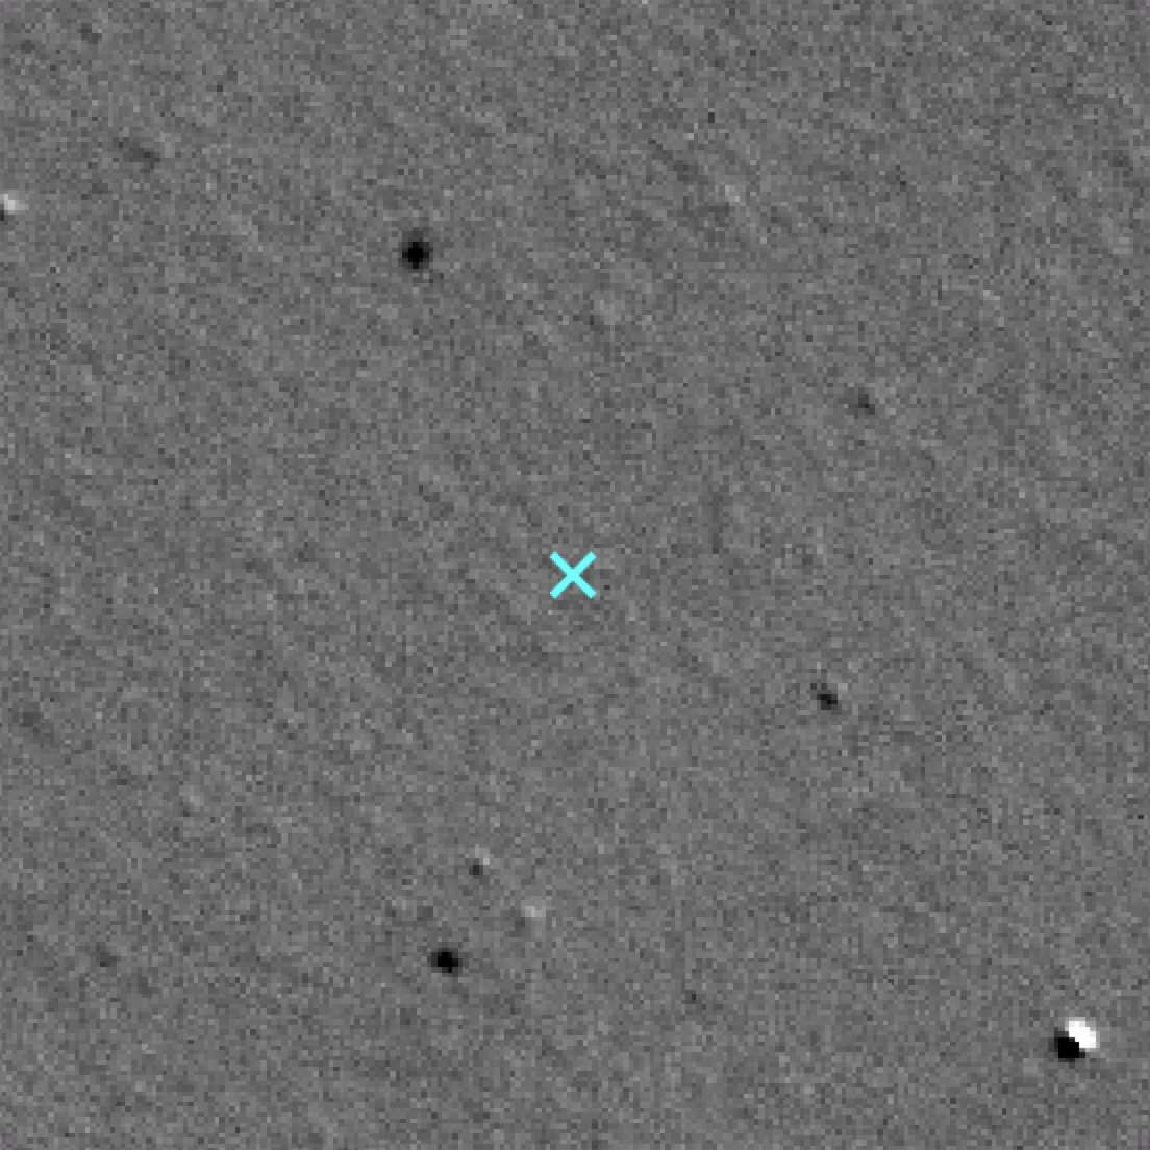
\includegraphics[width=.32\textwidth]{Figures/LGGS_2007_11f_OIII_sub_inverted_without_text.pdf}}
\caption{{\bf -- M\,31N 2007-11f}. The location of the nova (in field 6) is indicated by the blue cross. Left:\ Continuum subtracted LGGS H$\alpha$. Middle:\ Continuum subtracted LGGS [\ion{S}{ii}]. Right:\ Continuum subtracted LGGS [\ion{O}{iii}].}
\label{2007-11f surrounding sub images}
\end{figure*}

\begin{figure*}
\centering
\subfloat{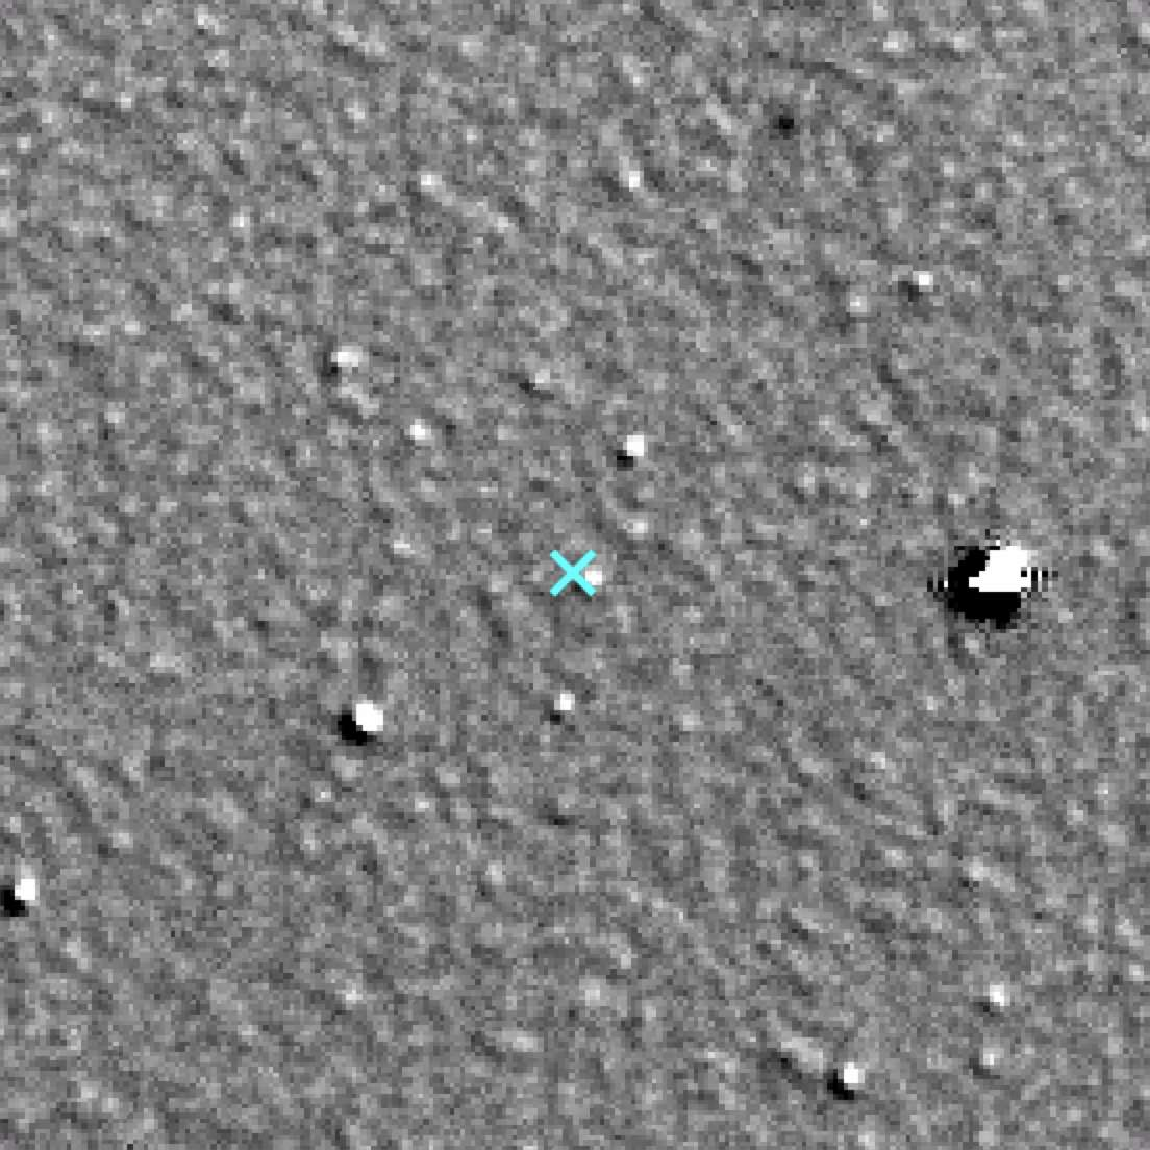
\includegraphics[width=.32\textwidth]{Figures/LGGS_1923_12c_Ha_sub_inverted_without_text.pdf}} \quad
\subfloat{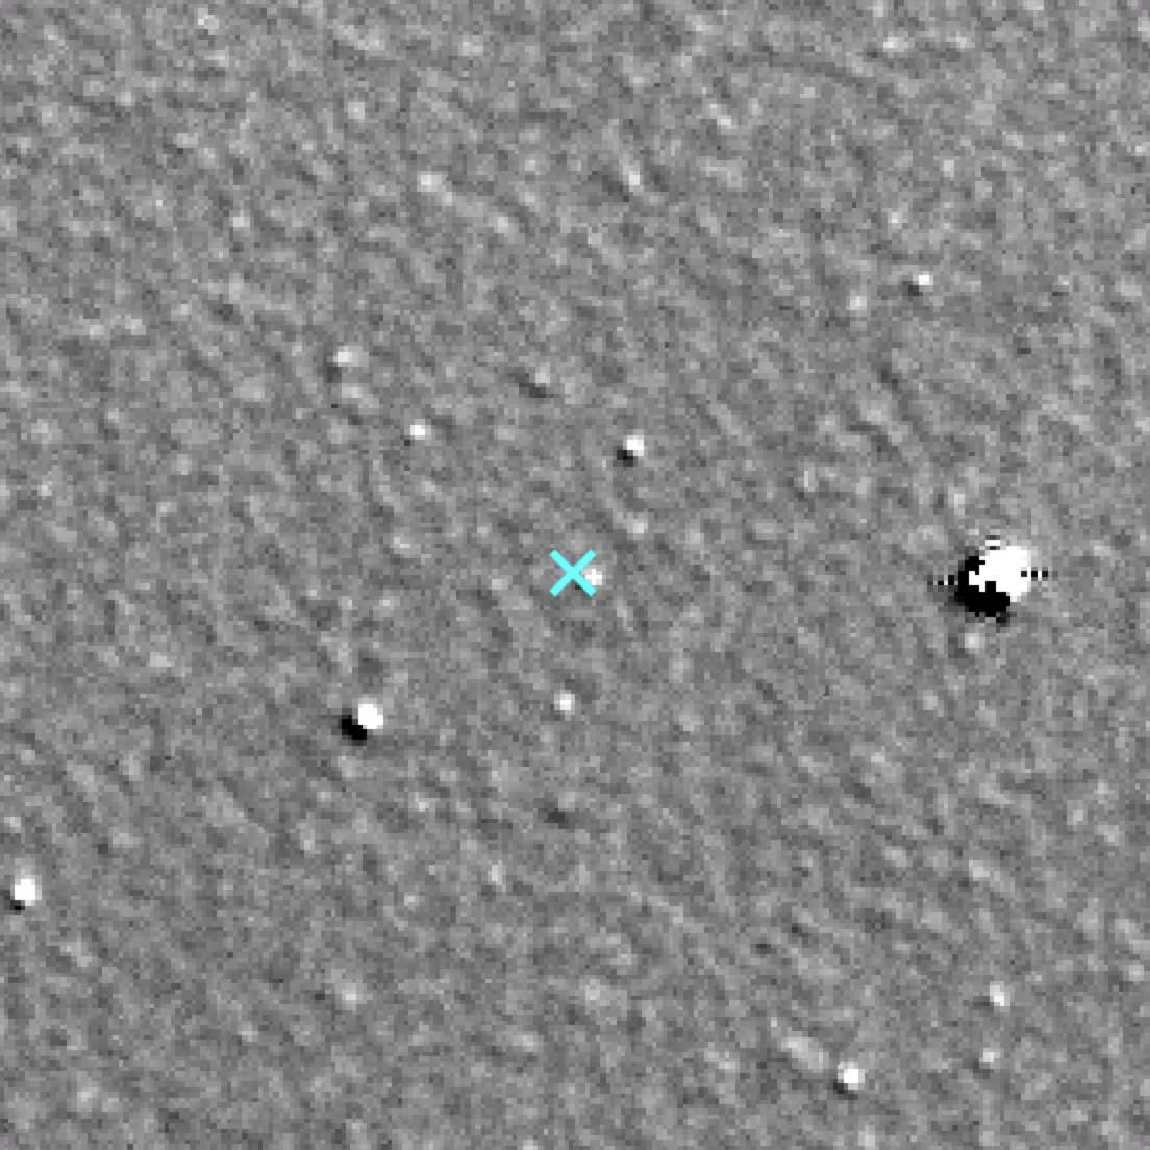
\includegraphics[width=.32\textwidth]{Figures/LGGS_1923_12c_SII_sub_inverted_without_text.pdf}} \quad
\subfloat{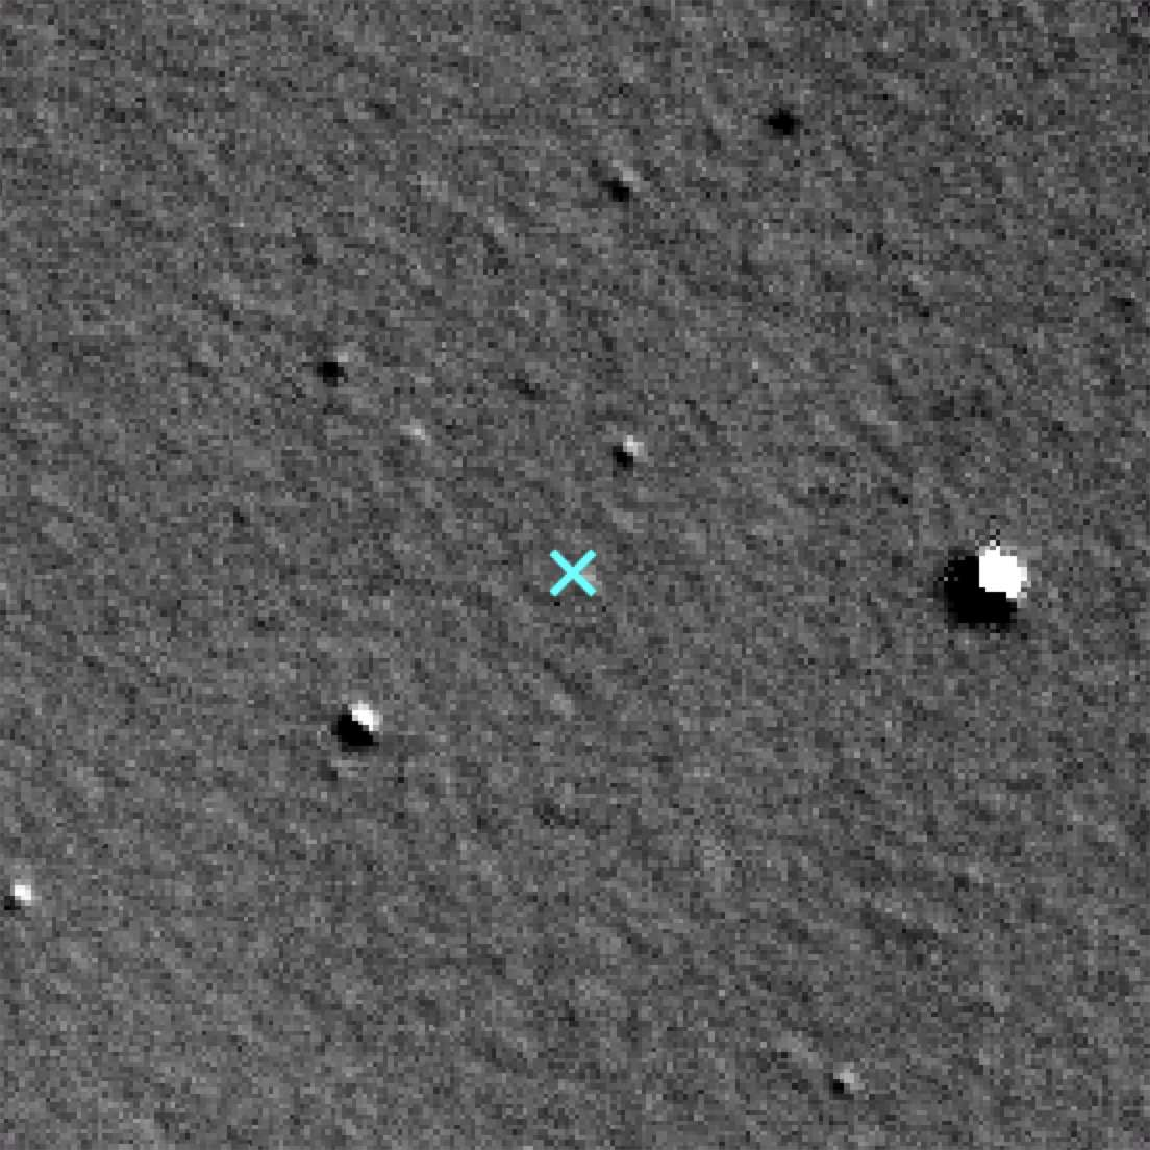
\includegraphics[width=.32\textwidth]{Figures/LGGS_1923_12c_OIII_sub_inverted_without_text.pdf}}
\caption{{\bf -- M\,31N 1923-12c}. The location of the nova (in field 6) is indicated by the blue cross. Left:\ Continuum subtracted LGGS H$\alpha$. Middle:\ Continuum subtracted LGGS [\ion{S}{ii}]. Right:\ Continuum subtracted LGGS [\ion{O}{iii}].}
\label{1923-12c surrounding sub images}
\end{figure*}

\begin{figure*}
\centering
\subfloat{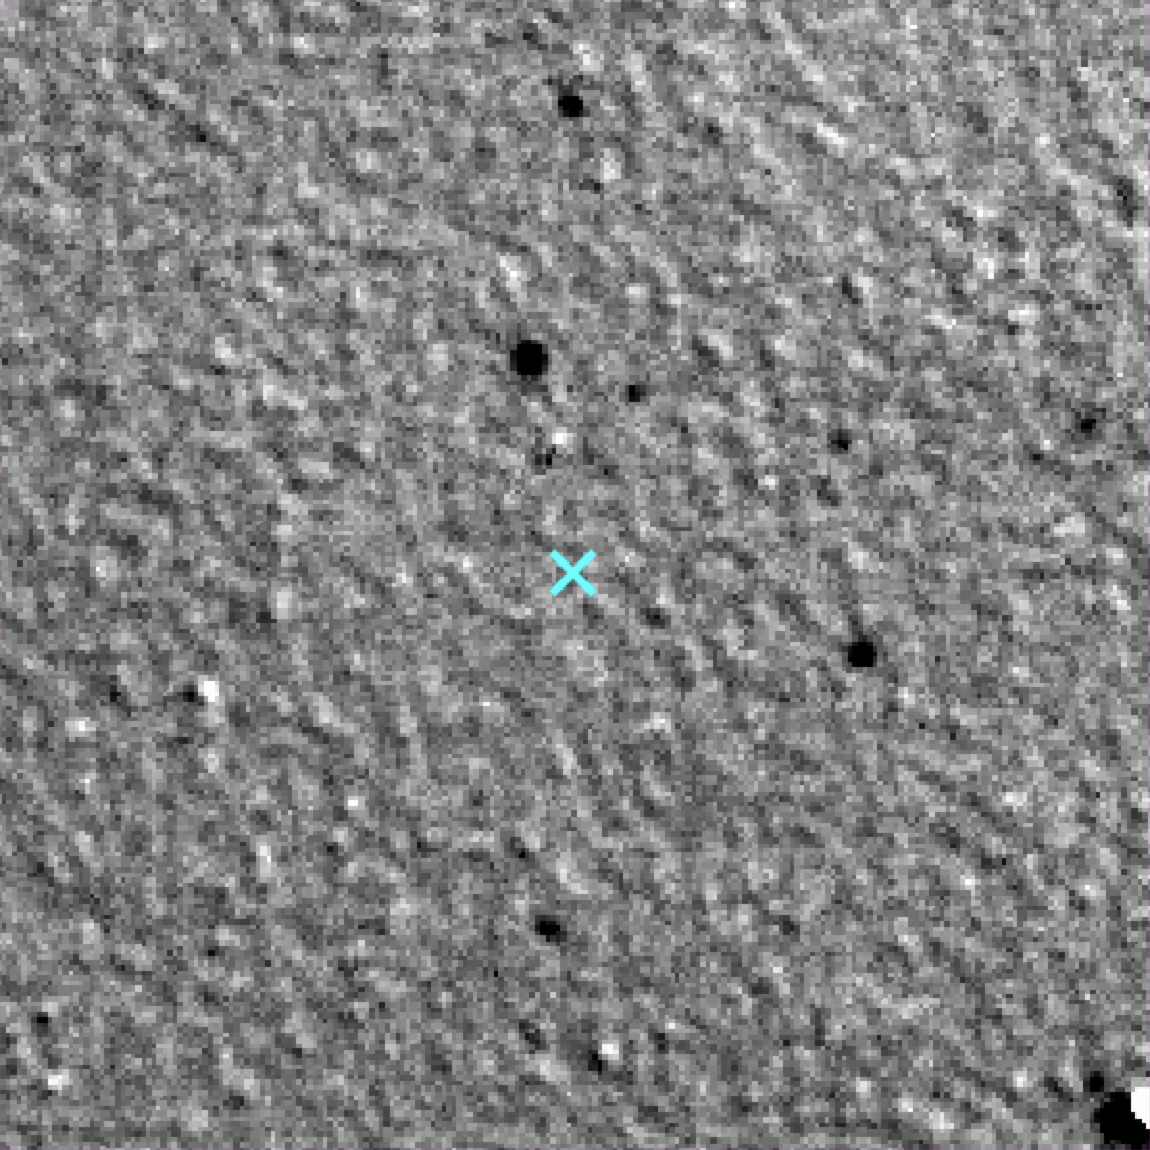
\includegraphics[width=.32\textwidth]{Figures/LGGS_2013_10c_Ha_sub_inverted_without_text.pdf}} \quad
\subfloat{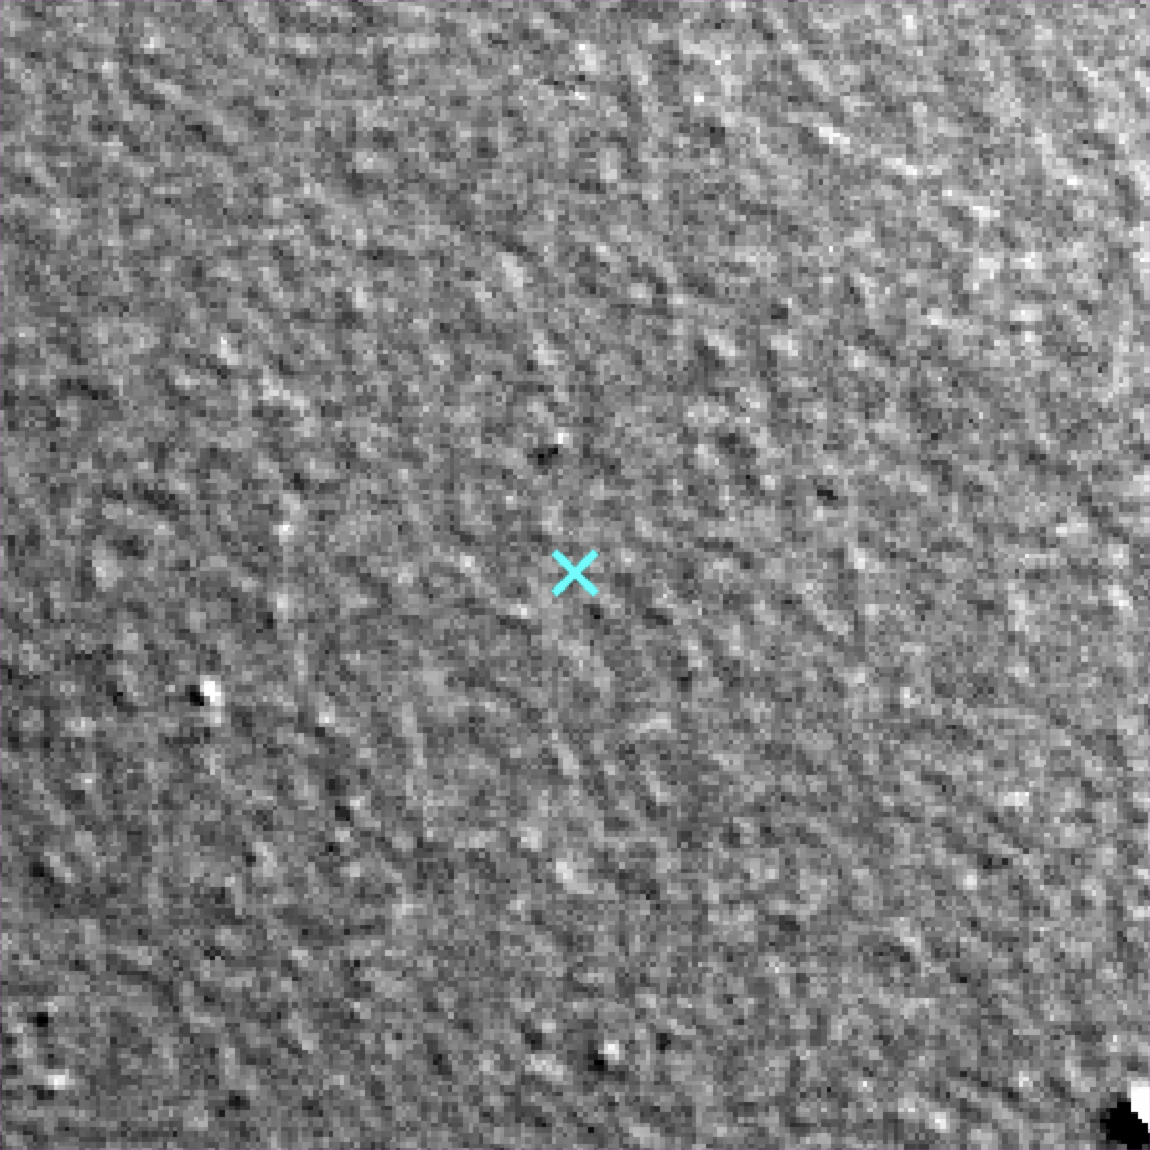
\includegraphics[width=.32\textwidth]{Figures/LGGS_2013_10c_SII_sub_inverted_without_text.pdf}} \quad
\subfloat{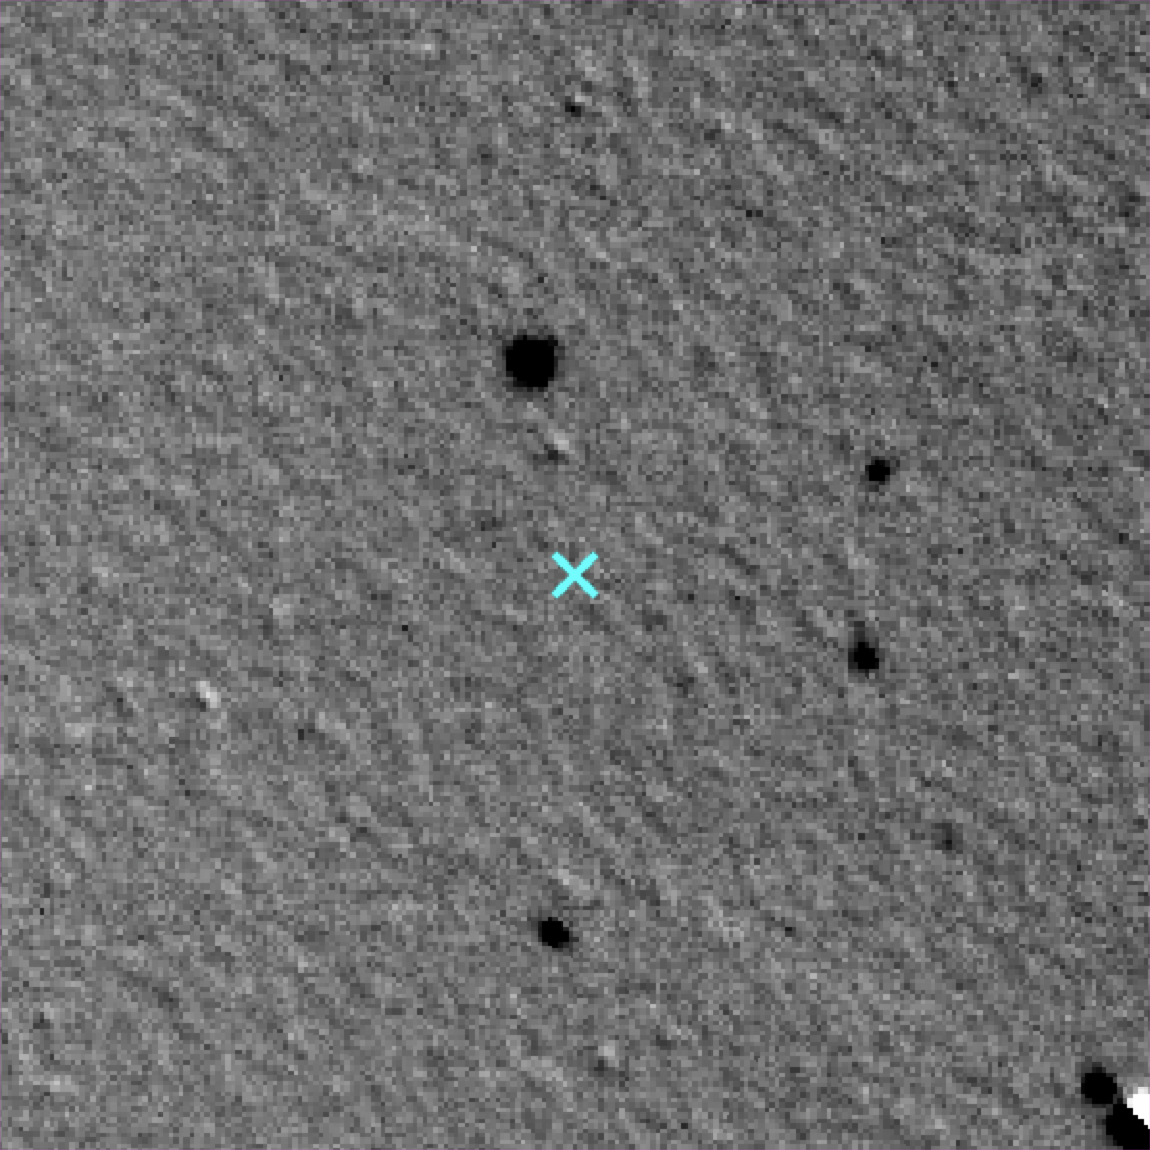
\includegraphics[width=.32\textwidth]{Figures/LGGS_2013_10c_OIII_sub_inverted_without_text.pdf}}
\caption{{\bf -- M\,31N 2013-10c}. The location of the nova (in field 6) is indicated by the blue cross. Left:\ Continuum subtracted LGGS H$\alpha$. Middle:\ Continuum subtracted LGGS [\ion{S}{ii}]. Right:\ Continuum subtracted LGGS [\ion{O}{iii}].}
\label{2013-10c surrounding sub images}
\end{figure*}

\begin{figure*}
\centering
\subfloat{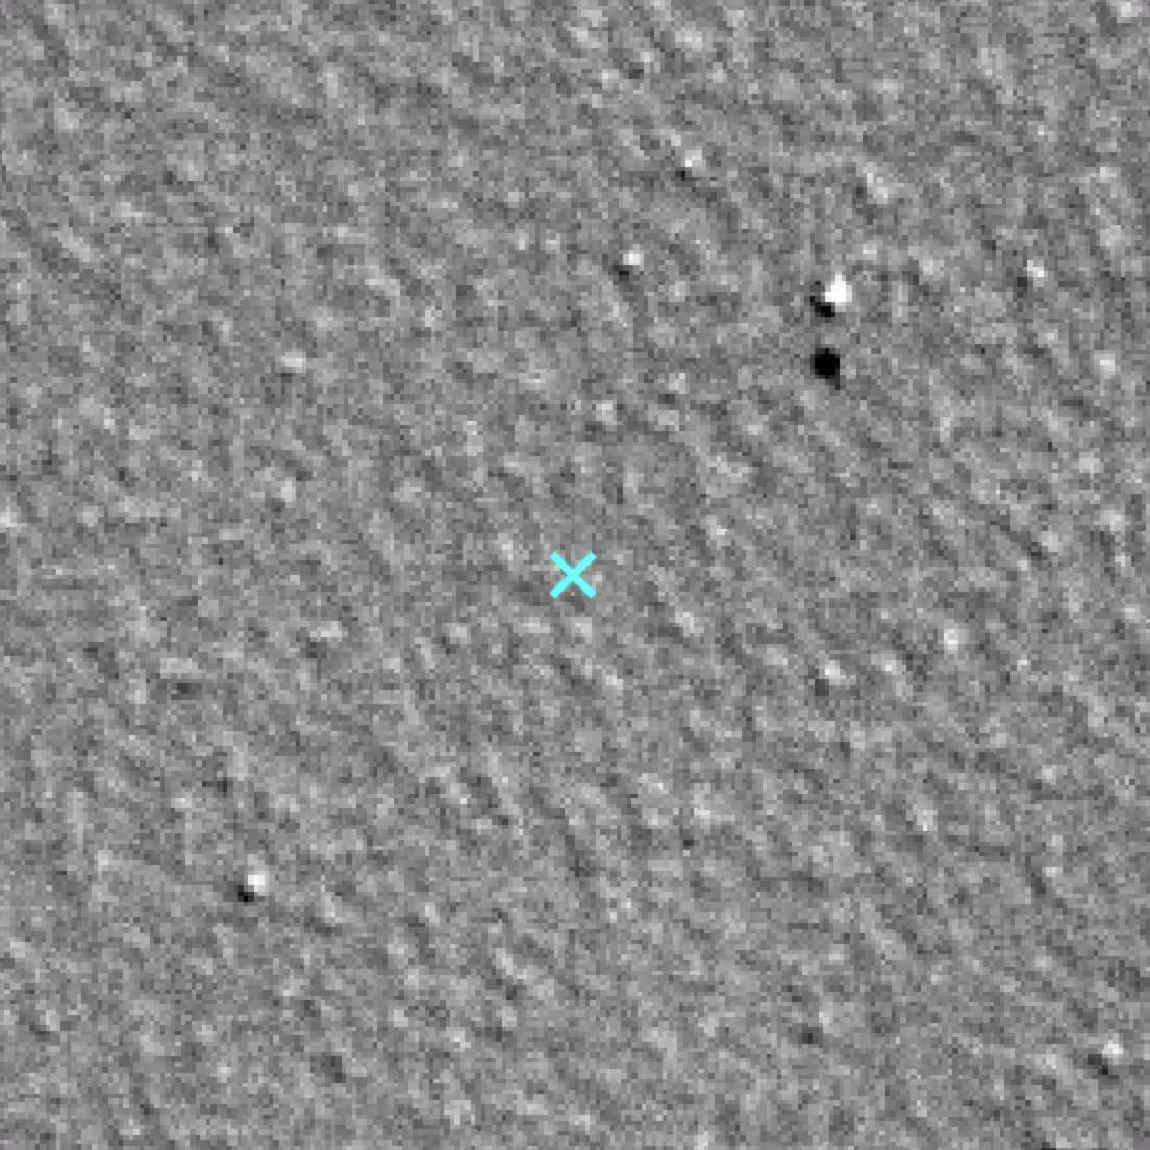
\includegraphics[width=.32\textwidth]{Figures/LGGS_2007_10b_Ha_sub_inverted_without_text.pdf}} \quad
\subfloat{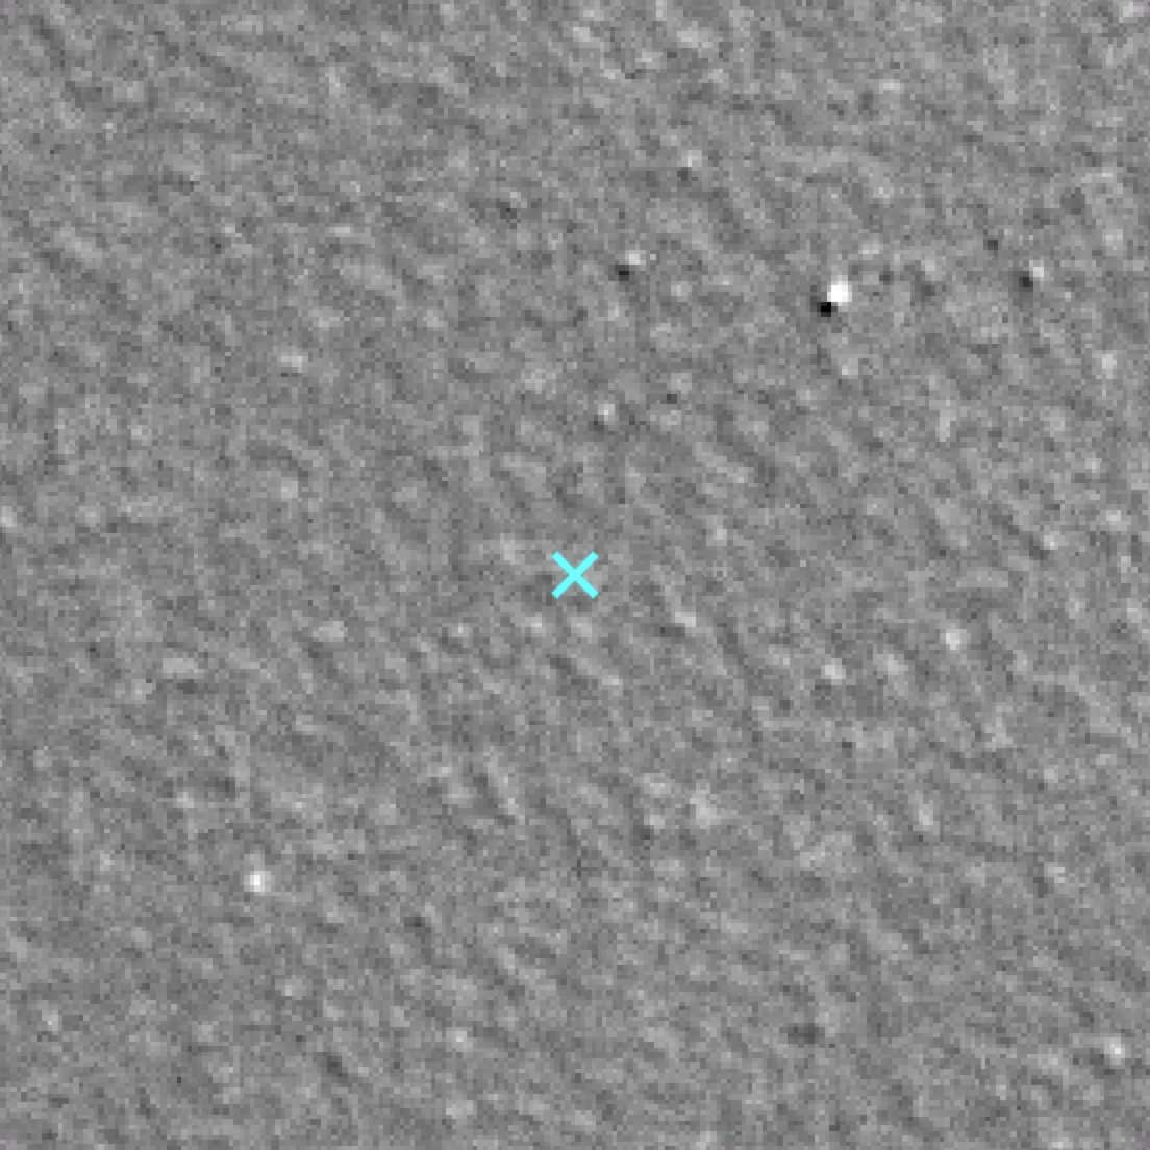
\includegraphics[width=.32\textwidth]{Figures/LGGS_2007_10b_SII_sub_inverted_without_text.pdf}} \quad
\subfloat{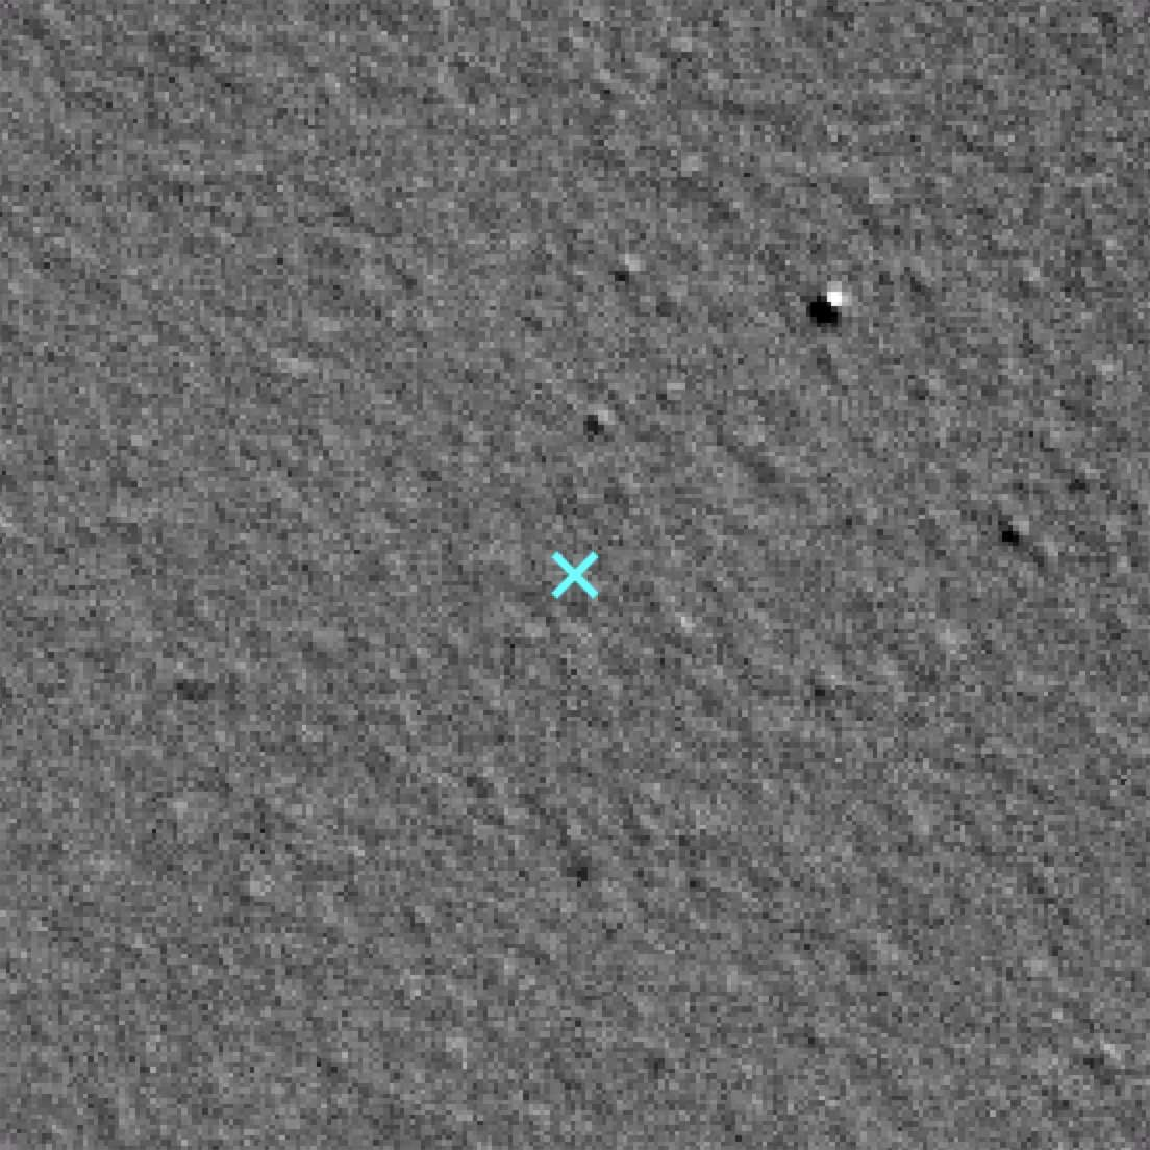
\includegraphics[width=.32\textwidth]{Figures/LGGS_2007_10b_OIII_sub_inverted_without_text.pdf}}
\caption{{\bf -- M\,31N 2007-10b}. The location of the nova (in field 6) is indicated by the blue cross. Left:\ Continuum subtracted LGGS H$\alpha$. Middle:\ Continuum subtracted LGGS [\ion{S}{ii}]. Right:\ Continuum subtracted LGGS [\ion{O}{iii}].}
\label{2007-10b surrounding sub images}
\end{figure*}

\begin{figure*}
\centering
\subfloat{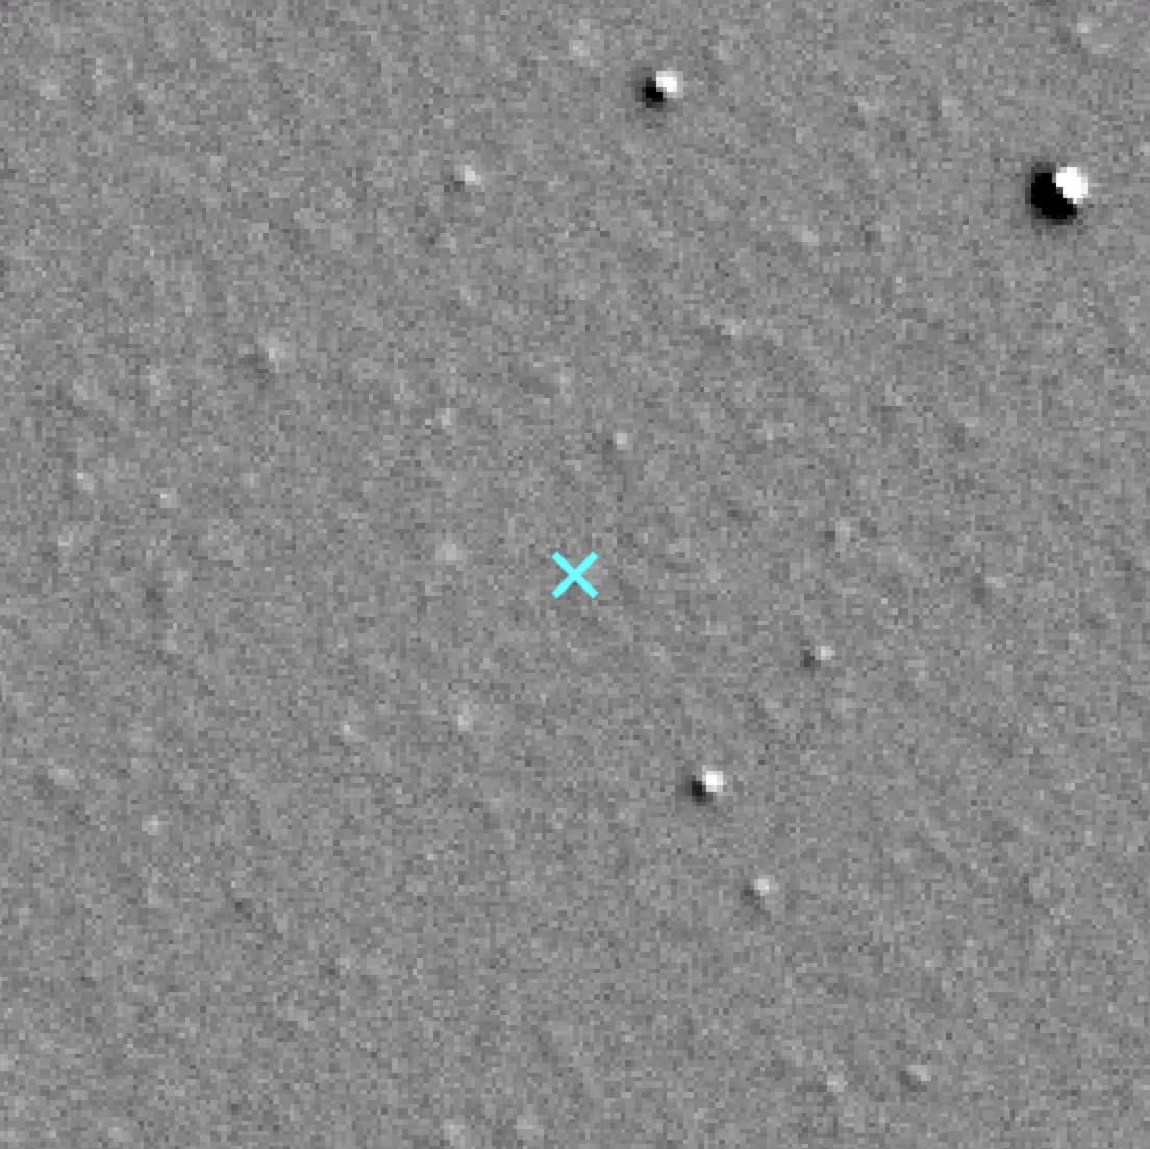
\includegraphics[width=.32\textwidth]{Figures/LGGS_1982_08b_Ha_sub_inverted_without_text.pdf}} \quad
\subfloat{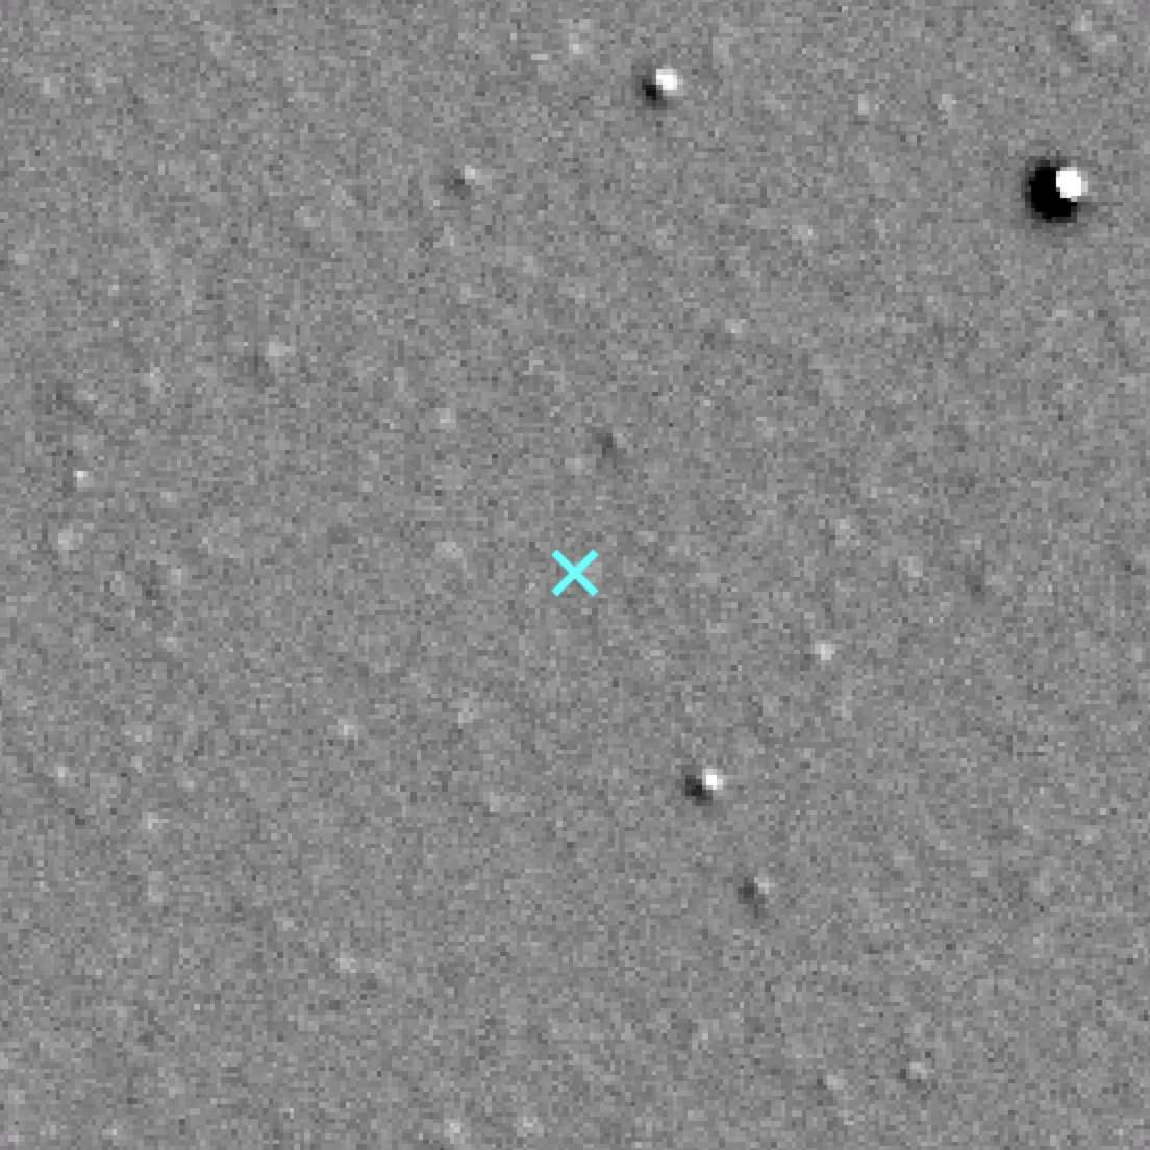
\includegraphics[width=.32\textwidth]{Figures/LGGS_1982_08b_SII_sub_inverted_without_text.pdf}} \quad
\subfloat{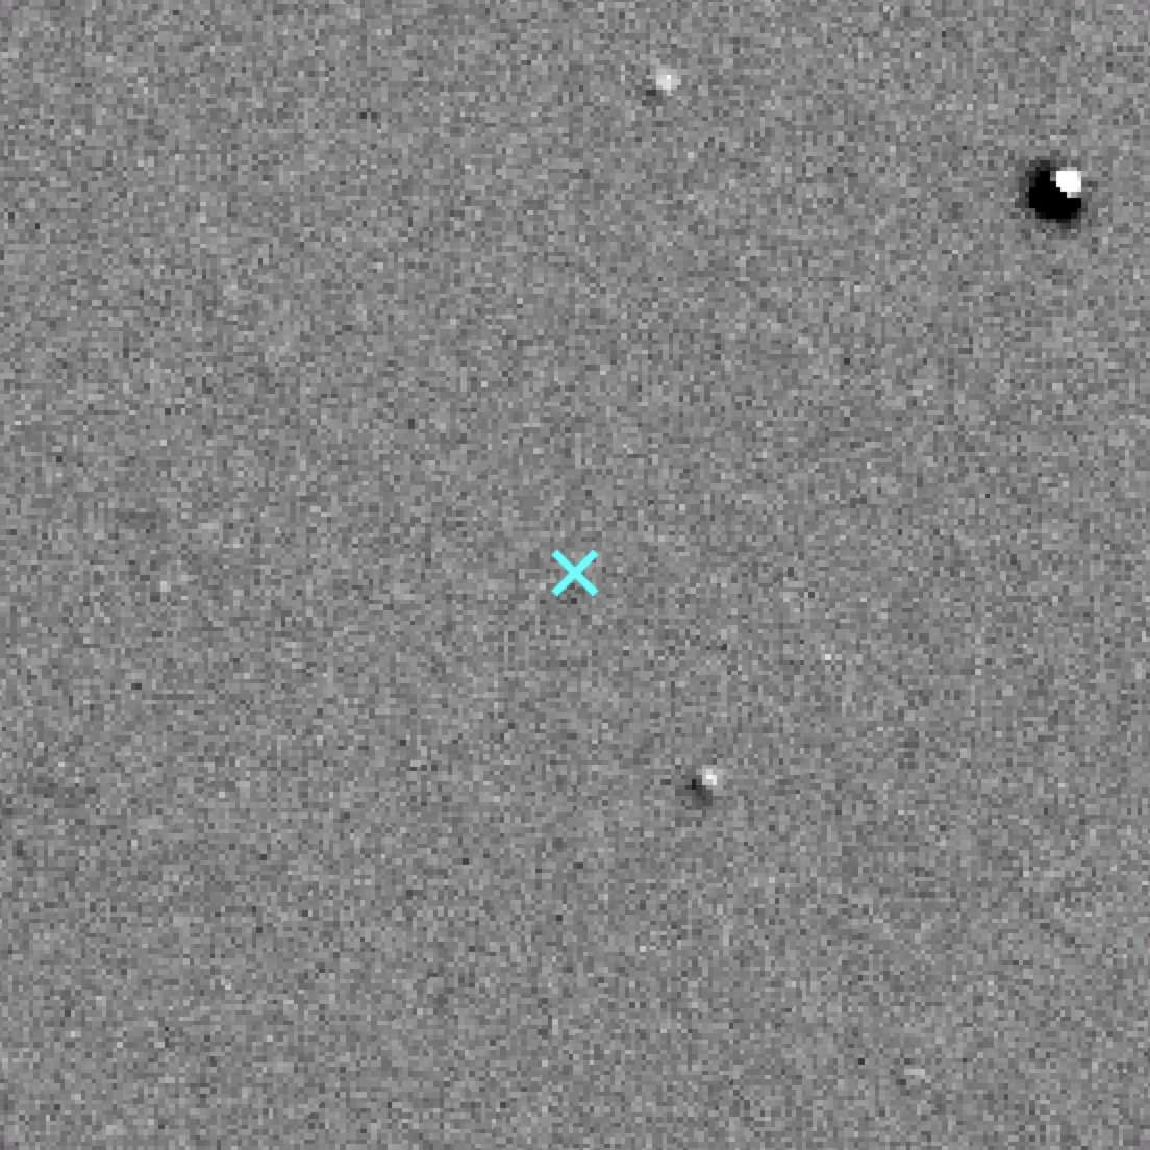
\includegraphics[width=.32\textwidth]{Figures/LGGS_1982_08b_OIII_sub_inverted_without_text.pdf}}
\caption{{\bf -- M\,31N 1982-08b}. The location of the nova (in field 3) is indicated by the blue cross. Left:\ Continuum subtracted LGGS H$\alpha$. Middle:\ Continuum subtracted LGGS [\ion{S}{ii}]. Right:\ Continuum subtracted LGGS [\ion{O}{iii}].}
\label{1982-08b surrounding sub images}
\end{figure*}

\begin{figure*}
\centering
\subfloat{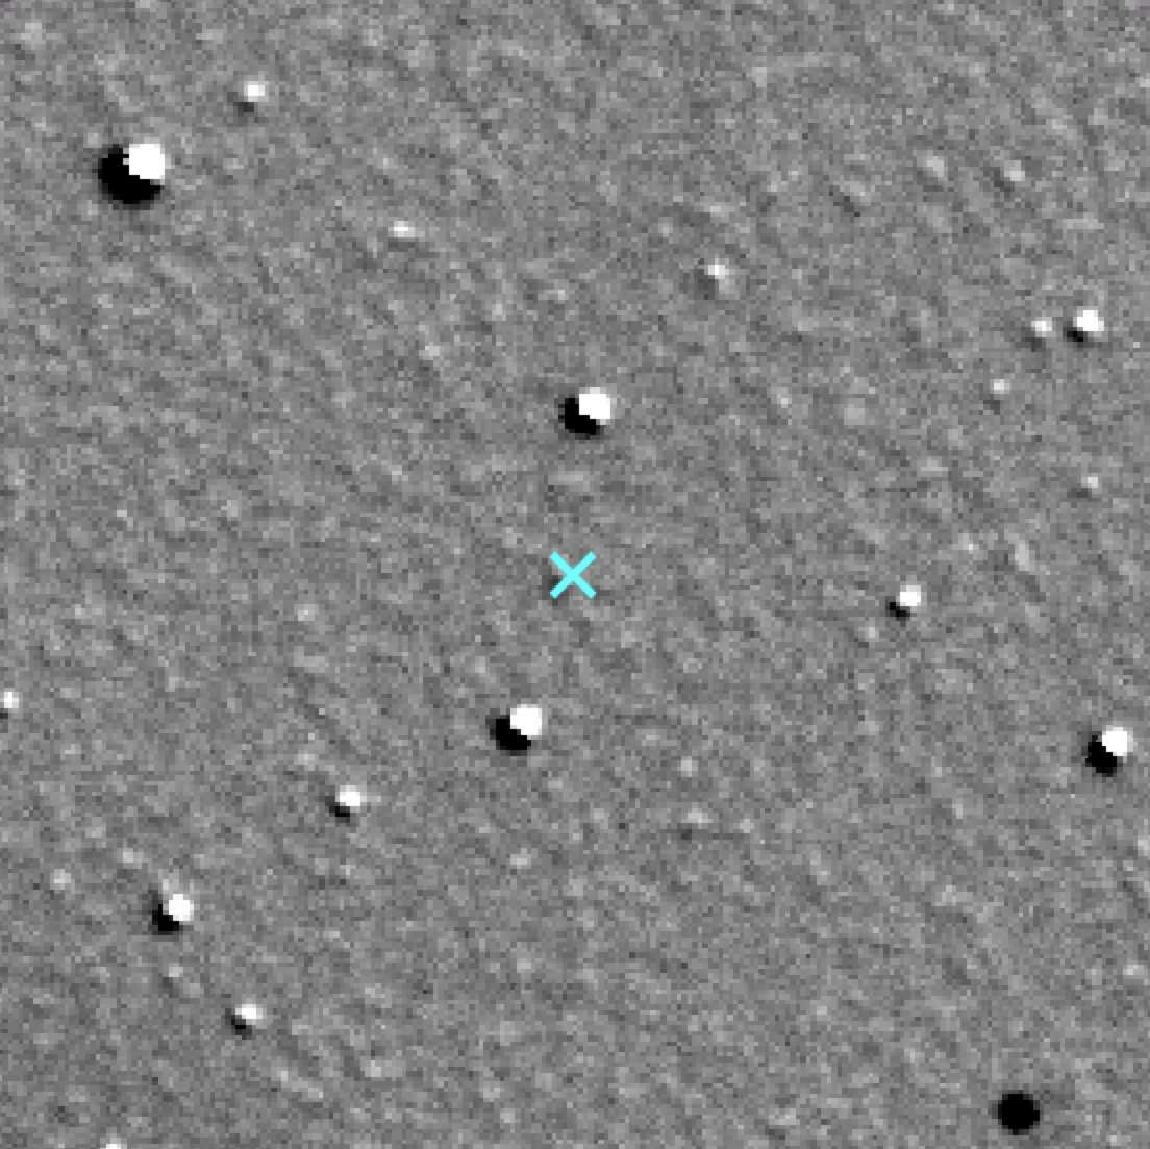
\includegraphics[width=.32\textwidth]{Figures/LGGS_1945_09c_Ha_sub_inverted_without_text.pdf}} \quad
\subfloat{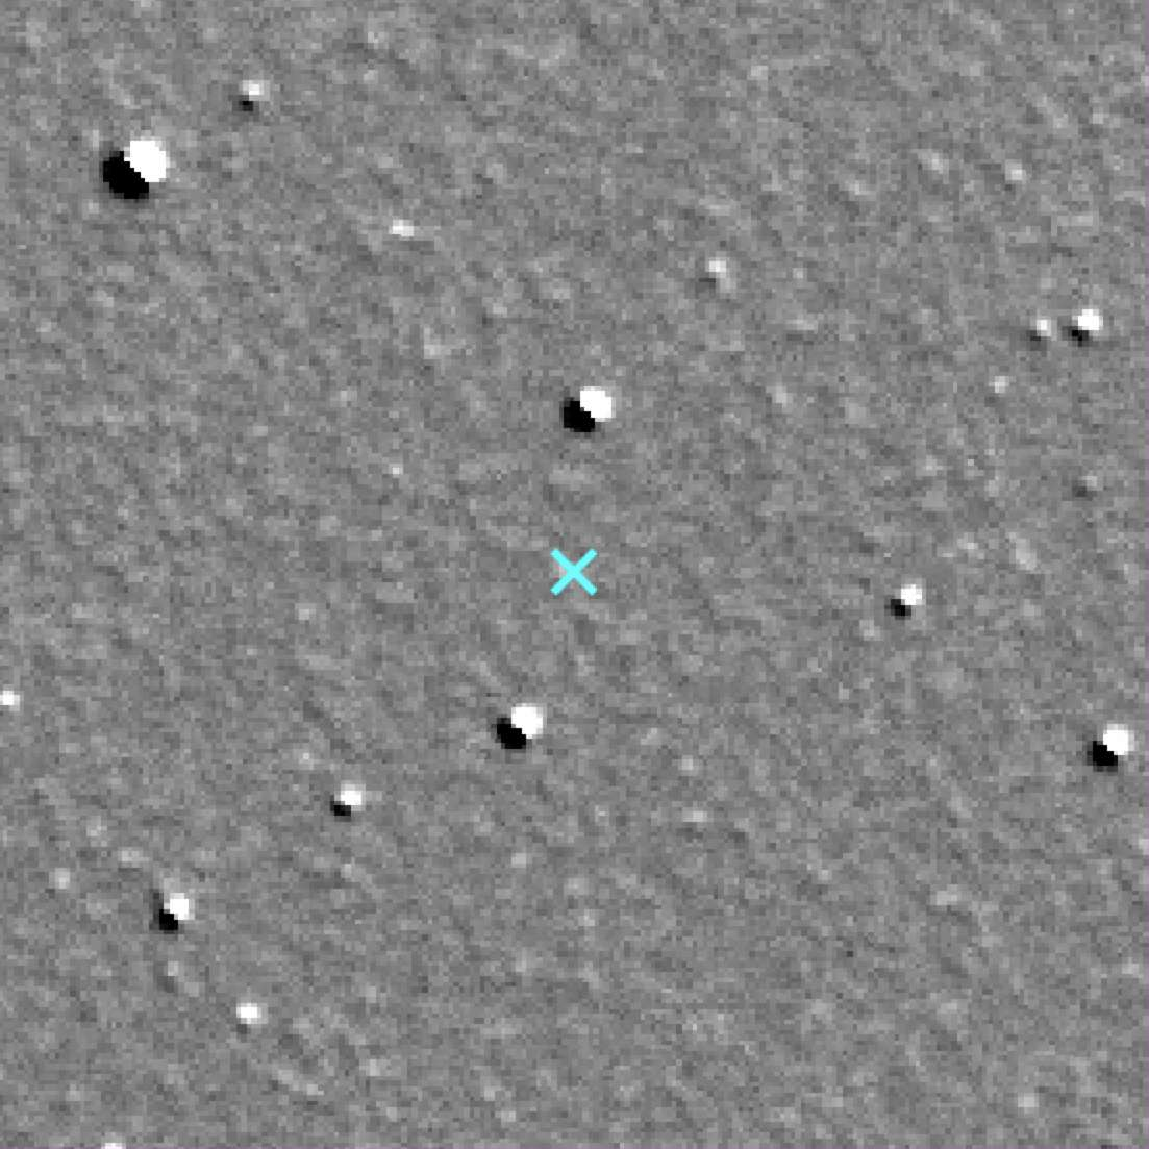
\includegraphics[width=.32\textwidth]{Figures/LGGS_1945_09c_SII_sub_inverted_without_text.pdf}} \quad
\subfloat{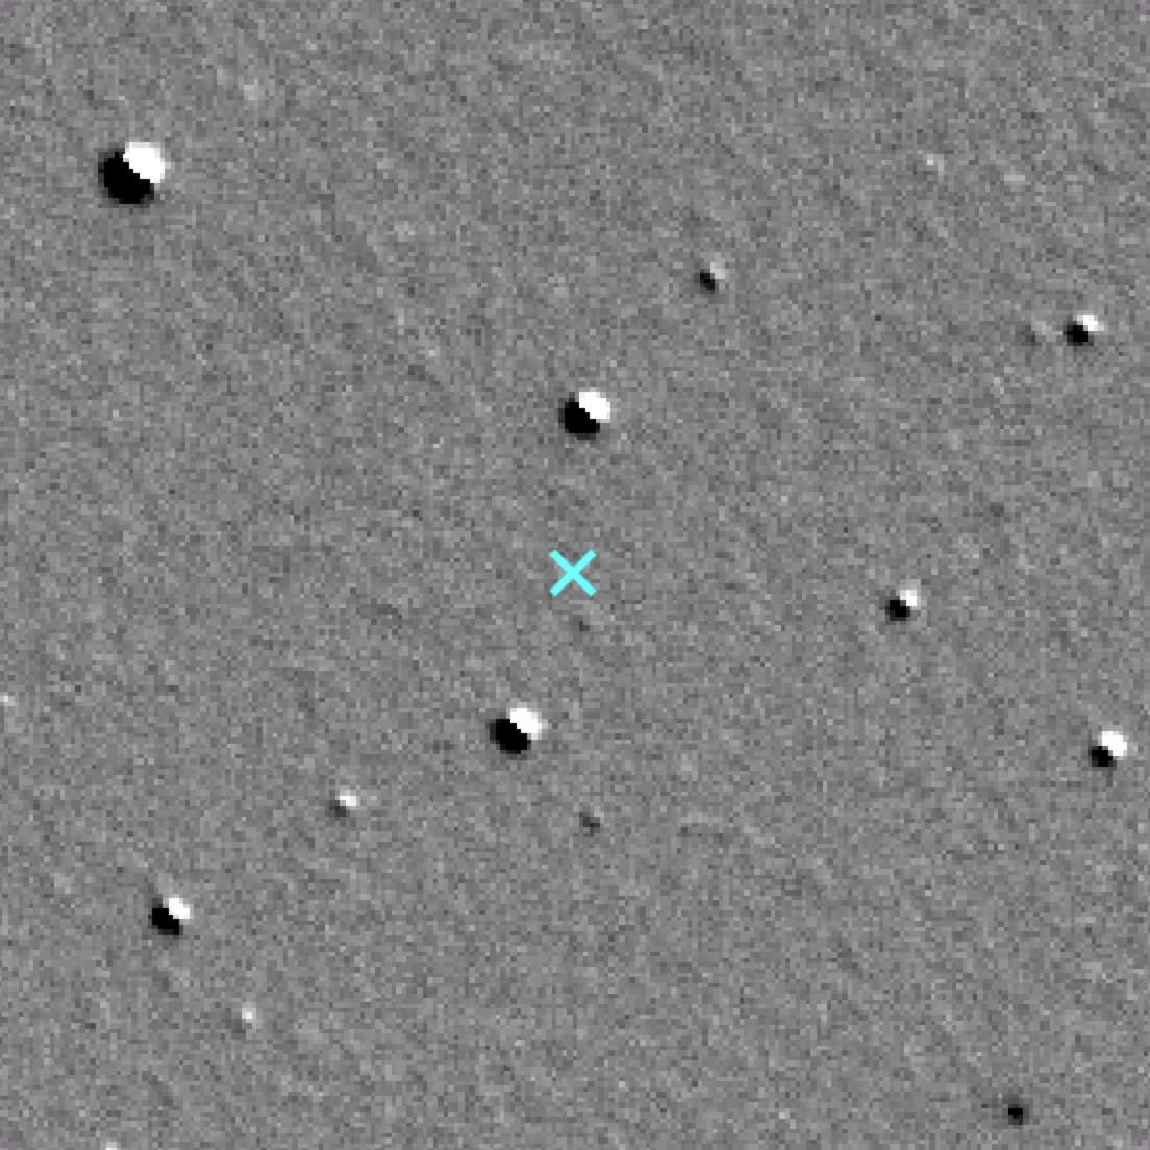
\includegraphics[width=.32\textwidth]{Figures/LGGS_1945_09c_OIII_sub_inverted_without_text.pdf}}
\caption{{\bf -- M\,31N 1945-09c}. The location of the nova (in field 6) is indicated by the blue cross. Left:\ Continuum subtracted LGGS H$\alpha$. Middle:\ Continuum subtracted LGGS [\ion{S}{ii}]. Right:\ Continuum subtracted LGGS [\ion{O}{iii}].}
\label{1945-09c surrounding sub images}
\end{figure*}

\begin{figure*}
\centering
\subfloat{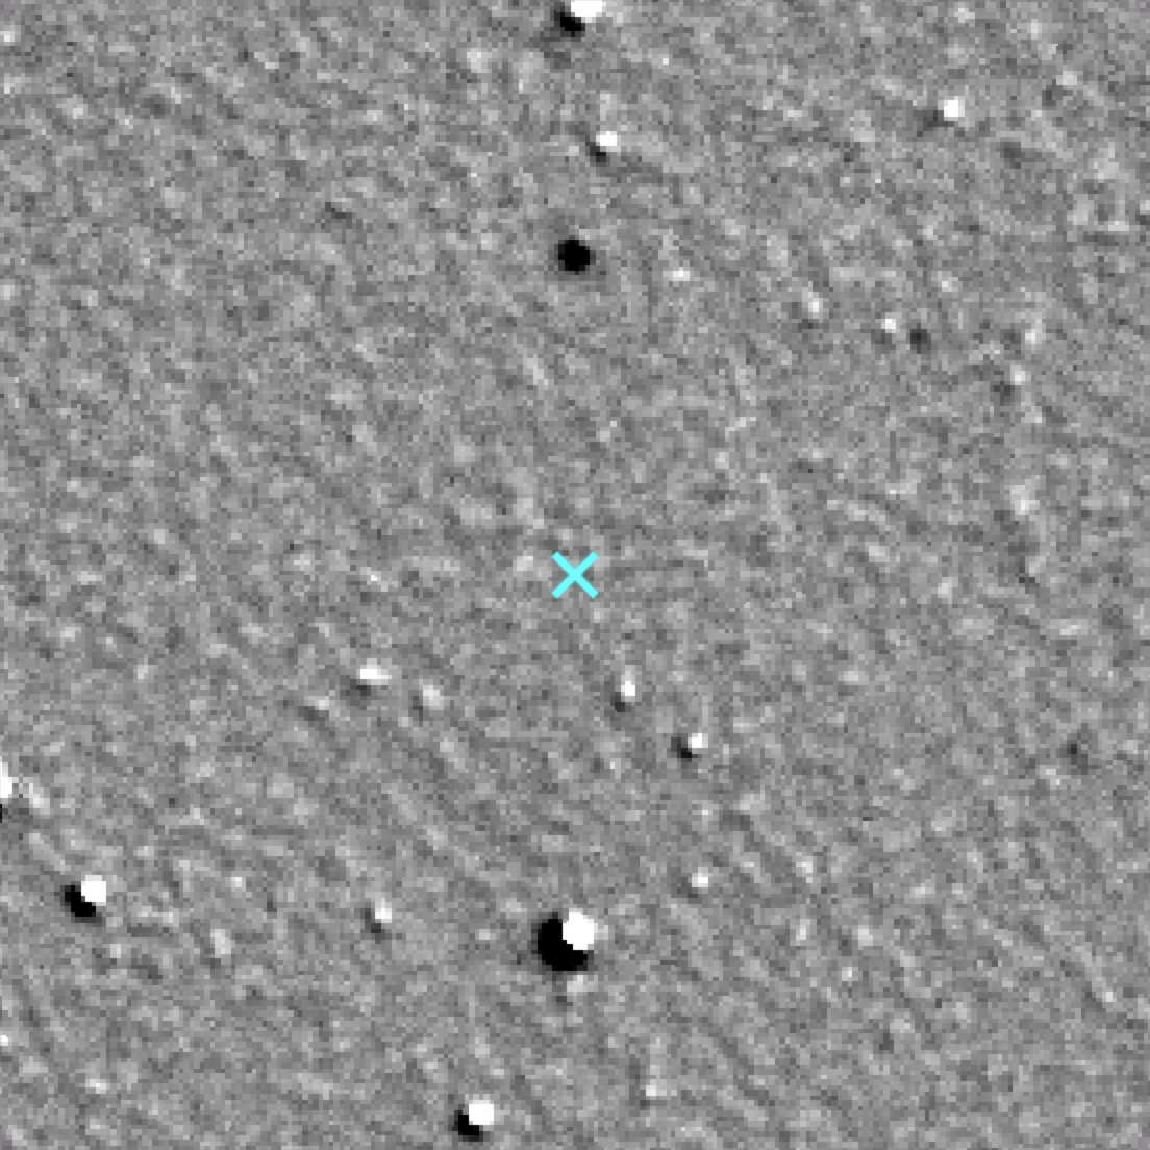
\includegraphics[width=.32\textwidth]{Figures/LGGS_1926_06a_Ha_sub_inverted_without_text.pdf}} \quad
\subfloat{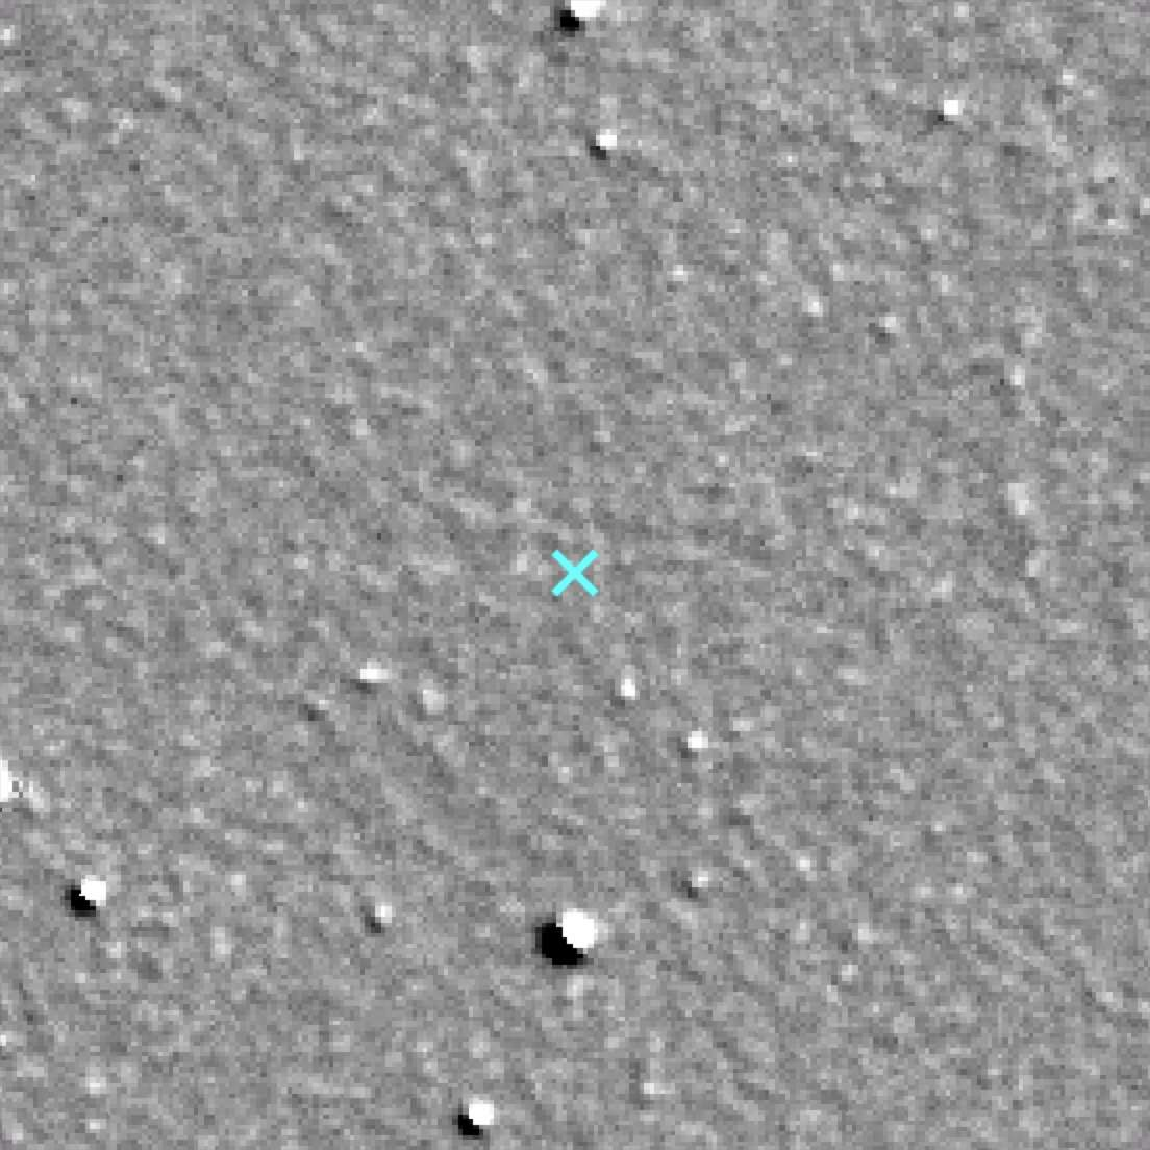
\includegraphics[width=.32\textwidth]{Figures/LGGS_1926_06a_SII_sub_inverted_without_text.pdf}} \quad
\subfloat{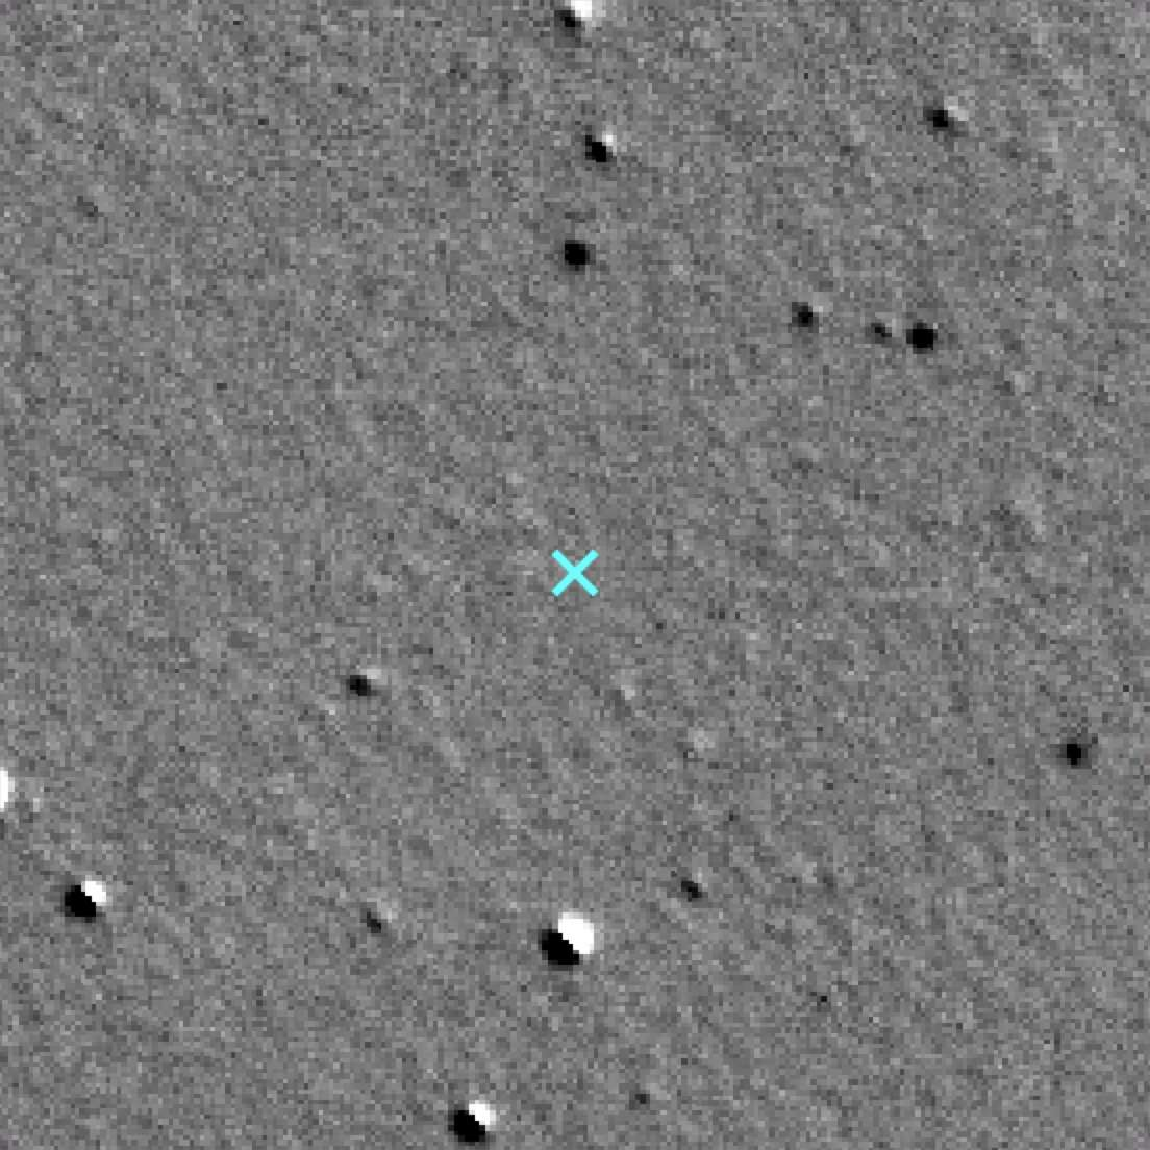
\includegraphics[width=.32\textwidth]{Figures/LGGS_1926_06a_OIII_sub_inverted_without_text.pdf}}
\caption{{\bf -- M\,31N 1926-06a}. The location of the nova (in field 6) is indicated by the blue cross. Left:\ Continuum subtracted LGGS H$\alpha$. Middle:\ Continuum subtracted LGGS [\ion{S}{ii}]. Right:\ Continuum subtracted LGGS [\ion{O}{iii}].}
\label{1926-06c surrounding sub images}
\end{figure*}

\begin{figure*}
\centering
\subfloat{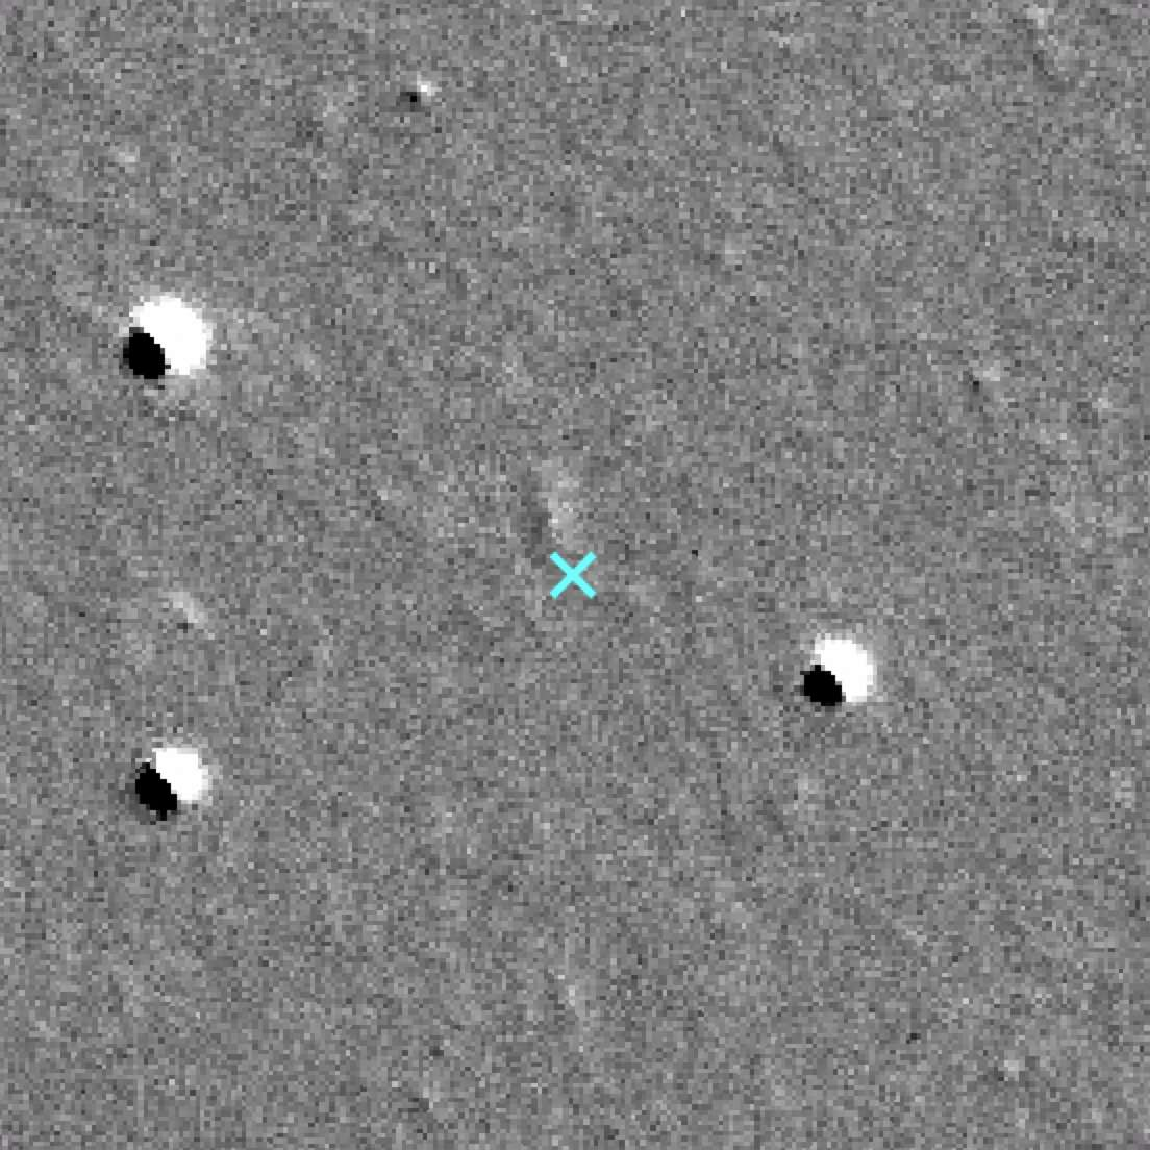
\includegraphics[width=.32\textwidth]{Figures/LGGS_1966_09e_Ha_sub_inverted_without_text.pdf}} \quad
\subfloat{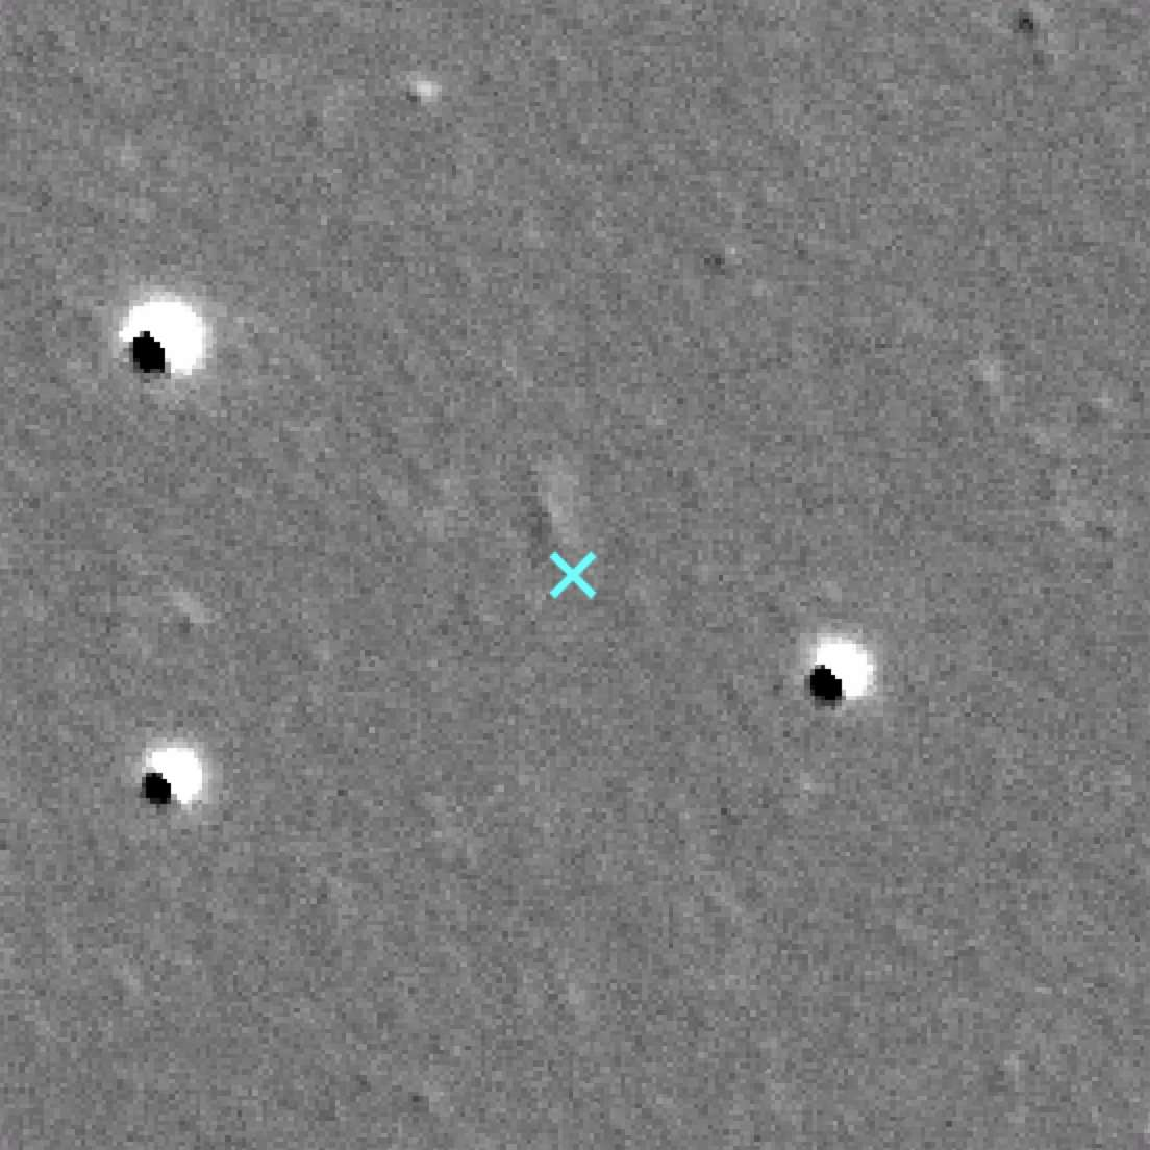
\includegraphics[width=.32\textwidth]{Figures/LGGS_1966_09e_SII_sub_inverted_without_text.pdf}} \quad
\subfloat{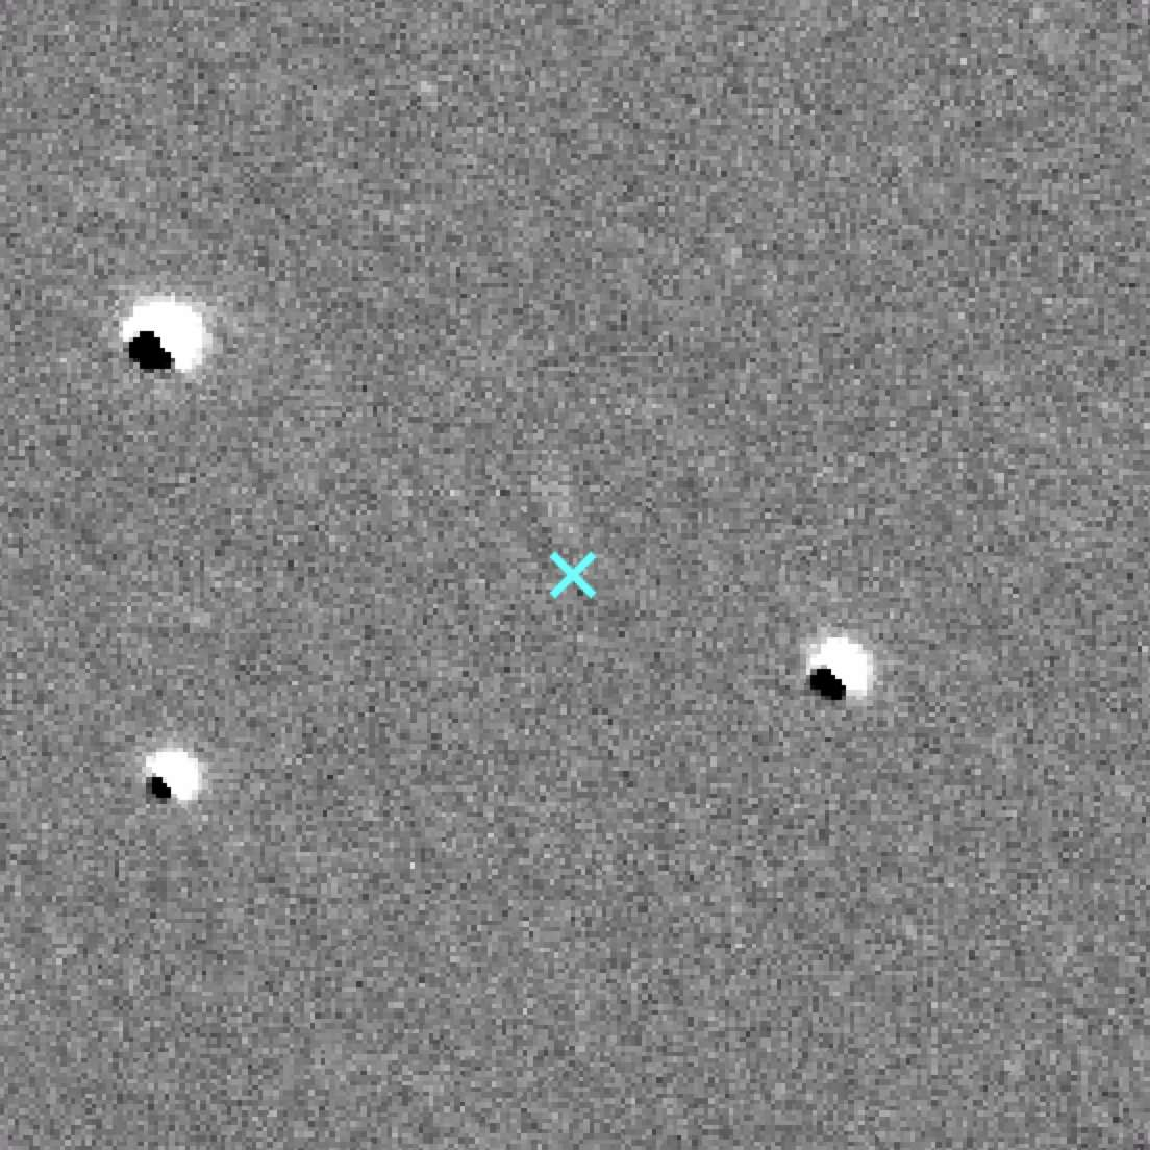
\includegraphics[width=.32\textwidth]{Figures/LGGS_1966_09e_OIII_sub_inverted_without_text.pdf}}
\caption{{\bf -- M\,31N 1966-09e}. The location of the nova (in field 8) is indicated by the blue cross. Left:\ Continuum subtracted LGGS H$\alpha$. Middle:\ Continuum subtracted LGGS [\ion{S}{ii}]. Right:\ Continuum subtracted LGGS [\ion{O}{iii}].}
\label{1966-09e surrounding sub images}
\end{figure*}

\begin{figure*}
\centering
\subfloat{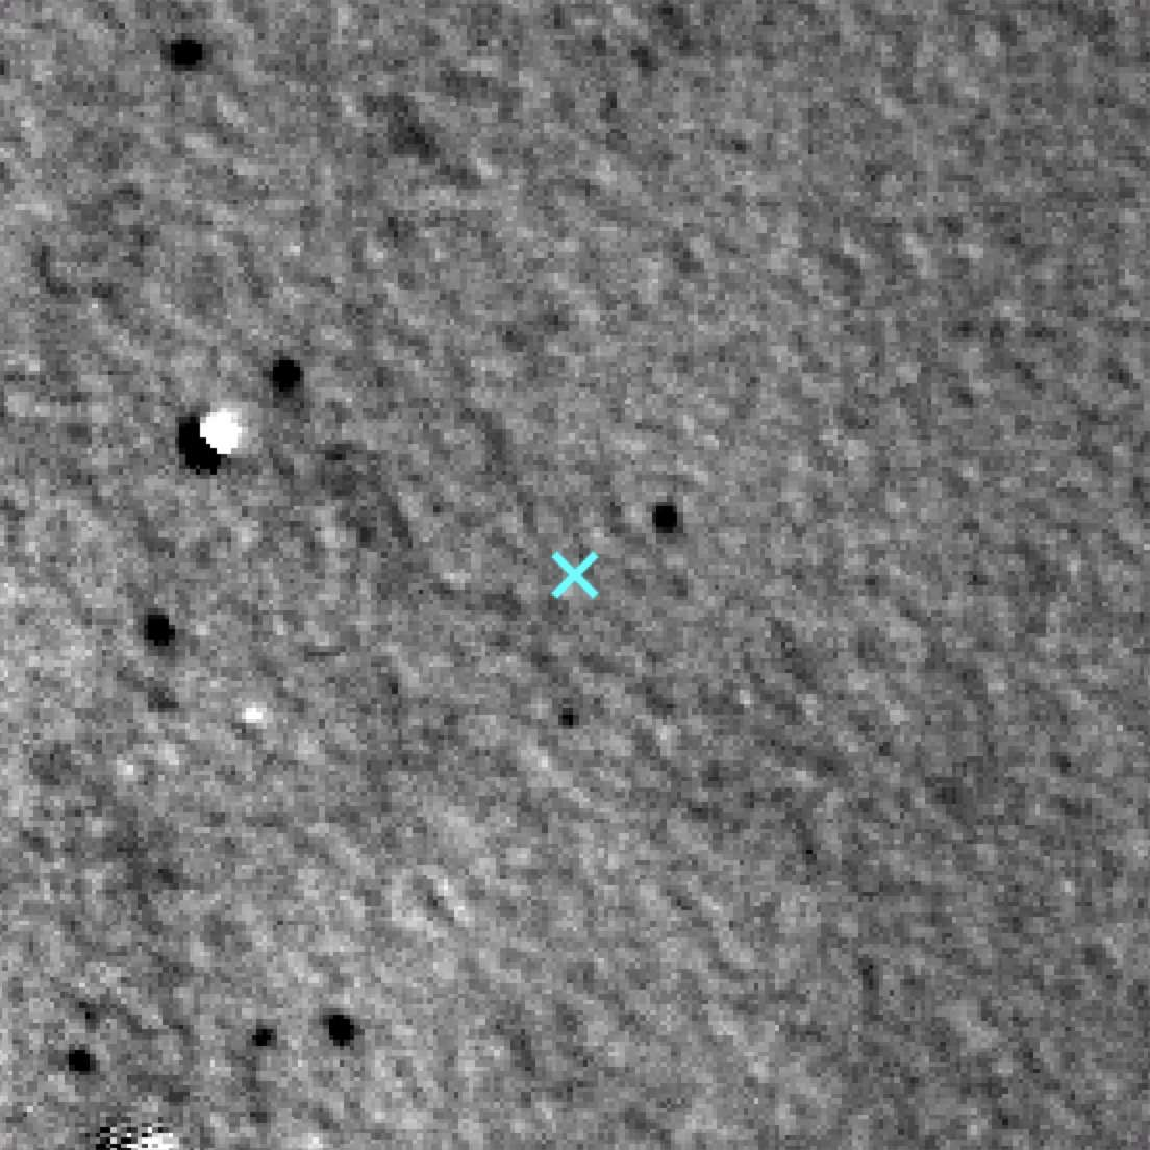
\includegraphics[width=.32\textwidth]{Figures/LGGS_1961_11a_Ha_sub_inverted_without_text.pdf}} \quad
\subfloat{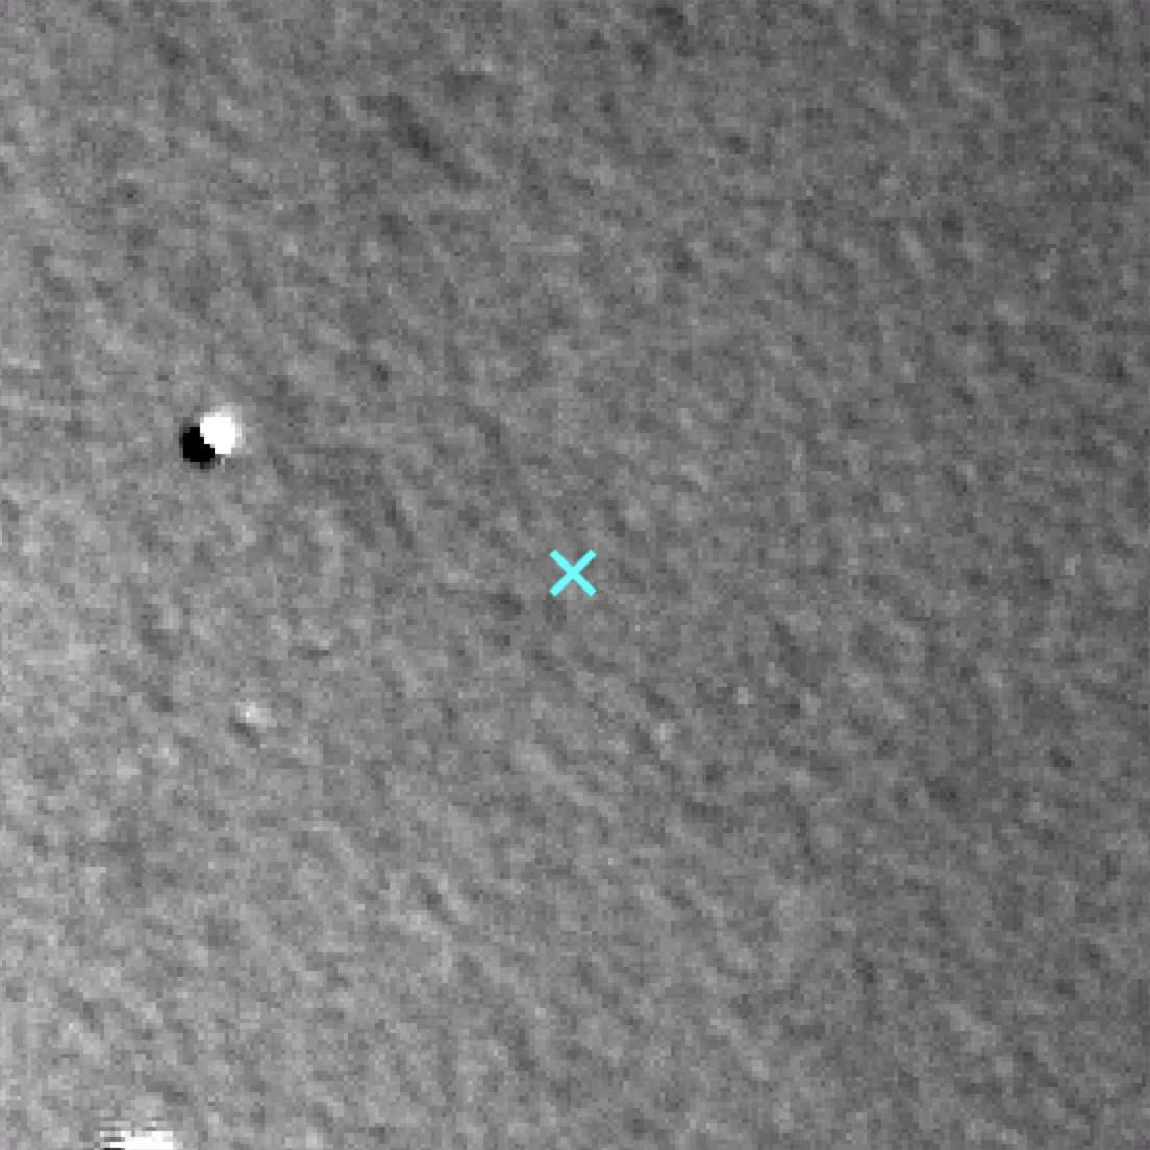
\includegraphics[width=.32\textwidth]{Figures/LGGS_1961_11a_SII_sub_inverted_without_text.pdf}} \quad
\subfloat{\includegraphics[width=.32\textwidth]{Figures/LGGS_1961_11a_OIII_sub_inverted_without_text.pdf}}
\caption{{\bf -- M\,31N 1961-11a}. The location of the nova (in field 6) is indicated by the blue cross. Left:\ Continuum subtracted LGGS H$\alpha$. Middle:\ Continuum subtracted LGGS [\ion{S}{ii}]. Right:\ Continuum subtracted LGGS [\ion{O}{iii}].}
\label{1961-11a surrounding sub images}
\end{figure*}

\begin{figure*}
\centering
\subfloat{\includegraphics[width=.32\textwidth]{Figures/LGGS_1953_09b_Ha_sub_inverted_without_text.pdf}} \quad
\subfloat{\includegraphics[width=.32\textwidth]{Figures/LGGS_1953_09b_SII_sub_inverted_without_text.pdf}} \quad
\subfloat{\includegraphics[width=.32\textwidth]{Figures/LGGS_1953_09b_OIII_sub_inverted_without_text.pdf}}
\caption{{\bf -- M\,31N 1953-09b}. The location of the nova (in field 6) is indicated by the blue cross. Left:\ Continuum subtracted LGGS H$\alpha$. Middle:\ Continuum subtracted LGGS [\ion{S}{ii}]. Right:\ Continuum subtracted LGGS [\ion{O}{iii}].}
\label{1953-09b surrounding sub images}
\end{figure*}

\begin{figure*}
\centering
\subfloat{\includegraphics[width=.32\textwidth]{Figures/LGGS_1919_09a_Ha_sub_inverted_without_text.pdf}} \quad
\subfloat{\includegraphics[width=.32\textwidth]{Figures/LGGS_1919_09a_SII_sub_inverted_without_text.pdf}} \quad
\subfloat{\includegraphics[width=.32\textwidth]{Figures/LGGS_1919_09a_OIII_sub_inverted_without_text.pdf}}
\caption{{\bf -- M\,31N 1919-09a}. The location of the nova (in field 6) is indicated by the blue cross. Left:\ Continuum subtracted LGGS H$\alpha$. Middle:\ Continuum subtracted LGGS [\ion{S}{ii}]. Right:\ Continuum subtracted LGGS [\ion{O}{iii}].}
\label{1919-09a surrounding sub images}
\end{figure*}

\begin{figure*}
\centering
\subfloat{\includegraphics[width=.32\textwidth]{Figures/FTS_1968_12a_Ha_inverted_without_text.pdf}} \quad
\subfloat{\includegraphics[width=.32\textwidth]{Figures/FTS_1968_12a_OIII_inverted_without_text.pdf}} \quad
\subfloat{\includegraphics[width=.32\textwidth]{Figures/Blank.pdf}}
\caption{{\bf -- LMCN 1968-12a}. The location of the nova is indicated by the blue cross. Left:\ Continuum subtracted FTS H$\alpha$. Right:\ Continuum subtracted FTS [\ion{O}{iii}].}
\label{LMCN 1968-12a surrounding sub images}
\end{figure*}

\begin{figure*}
\centering
\subfloat{\includegraphics[width=.32\textwidth]{Figures/FTS_1996_Ha_inverted_without_text.pdf}} \quad
\subfloat{\includegraphics[width=.32\textwidth]{Figures/FTS_1996_OIII_inverted_without_text.pdf}} \quad
\subfloat{\includegraphics[width=.32\textwidth]{Figures/Blank.pdf}}
\caption{{\bf -- LMCN 1996}. The location of the nova is indicated by the blue cross. Left:\ Continuum subtracted FTS H$\alpha$. Right:\ Continuum subtracted FTS [\ion{O}{iii}].}
\label{LMCN 1996 surrounding sub images}
\end{figure*}

\begin{figure*}
\centering
\subfloat{\includegraphics[width=.32\textwidth]{Figures/FTS_1971_08a_Ha_inverted_without_text.pdf}} \quad
\subfloat{\includegraphics[width=.32\textwidth]{Figures/FTS_1971_08a_OIII_inverted_without_text.pdf}} \quad
\subfloat{\includegraphics[width=.32\textwidth]{Figures/Blank.pdf}}
\caption{{\bf -- LMCN 1971-08a}. The location of the nova is indicated by the blue cross. Left:\ Continuum subtracted FTS H$\alpha$. Right:\ Continuum subtracted FTS [\ion{O}{iii}].}
\label{LMCN 1971-08a surrounding sub images}
\end{figure*}

\begin{figure*}
\centering
\subfloat{\includegraphics[width=.32\textwidth]{Figures/FTS_YY_Doradus_Ha_inverted_without_text.pdf}} \quad
\subfloat{\includegraphics[width=.32\textwidth]{Figures/FTS_YY_Doradus_OIII_inverted_without_text.pdf}} \quad
\subfloat{\includegraphics[width=.32\textwidth]{Figures/Blank.pdf}}
\caption{{\bf -- YY Doradus}. The location of the nova is indicated by the blue cross. Left:\ Continuum subtracted FTS H$\alpha$. Right:\ Continuum subtracted FTS [\ion{O}{iii}].}
\label{YY Doradus surrounding sub images}
\end{figure*}

\end{document}